\documentclass{beamer}
\usepackage{amssymb,amsmath}
\usepackage{graphicx}
\usepackage{listings}
\usepackage{xcolor}
\usepackage{algorithm}
\usepackage{algpseudocode}
 \setbeamertemplate{navigation symbols}{} 
 \renewcommand{\vec}[1]{\boldsymbol{#1}}

\definecolor{codegreen}{rgb}{0,0.6,0}
\definecolor{codegray}{rgb}{0.5,0.5,0.5}
\definecolor{codeblue}{rgb}{0,0,1}
\definecolor{codered}{rgb}{1.0,0,0}
\definecolor{backcolour}{rgb}{0.95,0.95,0.92}

\lstset{language=Python, 
    basicstyle=\footnotesize\ttfamily, 
    keywordstyle=\color{codegreen},
    commentstyle=\color{codegray},
    stringstyle=\color{codered},
    showstringspaces=false,
    identifierstyle=\color{codeblue},
    numbers=none,
}

\begin{document}

\begin{frame}
  \begin{center}
  \Large{MA32070/MA40177 Scientific Computing}
  \end{center}
  \vfill
  \footnotesize{
  These notes are copyright of Eike Mueller, University of Bath 2025. They are provided exclusively for educational purposes at the University and are to be downloaded or copied for your private study only. Further distribution, e.g. by upload to external repositories, is prohibited.}
\end{frame}

\section{Housekeeping}

%%%%%%%%%%%%%%%%%%%%%%%%%%%%%%%%%%%%%%%%%%%%%%%%%%%%%%%%%%%%%%%%%%

\begin{frame}
  \tableofcontents[currentsection]
\end{frame}

\begin{frame}
  \frametitle{Contact hours}
\textbf{Unit convenor}\\
  Eike Mueller, 4 West 2.17, \texttt{e.mueller@bath.ac.uk}\\
  Office hour: Tuesday 11:15h - 12:05h\\[2ex]
\textbf{Lectures/computer labs}

\begin{itemize} 
  \item 2 hour session every Tuesday 14:15h - 16:05h
  \item location: EB 0.9
  \item mixture of lectures and labs, varying throughout the semester
  \item recorded on Panopto {\footnotesize (let me know if you have any issues with this)}
\end{itemize}

Please\dots
\begin{itemize}
  \item \dots attend in person
  \item \dots ask questions at any point
\end{itemize}

\textbf{Lecture notes + slides} $\Rightarrow$ moodle\\[1ex]
Please email me if you spot any typos
\end{frame}

\begin{frame}
\frametitle{Intended learning outcomes}
\textbf{What will you learn?}
\begin{itemize}
  \item develop the coding skills necessary for the computational solution of challenging scientific and engineering problems
  \item learn how to use suitable software abstractions and libraries
  \item implement code in an efficient and sustainable way
  \item Gain an understanding of
  \begin{itemize}
    \item modern programming techniques and
    \item parallel computing architectures 
  \end{itemize}  
  \item understand different sources of error
  \item analyse performance of code
\end{itemize}
\textbf{How will you learn this?}
\begin{center}
  Implement Finite Element Method for elliptic problems in 2 dimensions
\end{center}
\end{frame}

%%%%%%%%%%%%%%%%%%%%%%%%%%%%%%%%%%%%%%%%%%%%%%%%%%%%%%%%%%%%%%%%%%

\begin{frame}
\frametitle{Assessment \& problem sheets}
\textbf{Summative assessment}
\begin{itemize}
\item 1 piece of coursework = 100\% of module mark
\item two weeks to complete the coursework assignment
\item mixture of implementation task and mathematical derivations
\item due in week 11
\end{itemize}
\vspace{2ex}
\textbf{Problem sheets (= formative assessment)}
\begin{itemize}
  \item available on moodle page
  \item write Python code + run numerical experiments
  \item \textbf{very important that you engage with these exercises}\\
   $\Rightarrow$ will make the coursework much easier!
  \item submit you solutions on moodle to get feedback\\
  \textbf{follow detailed submission instructions}
  \item model solutions on moodle (\textbf{but first try yourself})
\end{itemize}
\end{frame}

%%%%%%%%%%%%%%%%%%%%%%%%%%%%%%%%%%%%%%%%%%%%%%%%%%%%%%%%%%%%%%%%%%

\begin{frame}[fragile]
\frametitle{Programming in Python}
Default setup:
\begin{center}
\textbf{Notable + VSCode notebook}\\(= ``Standard Python 3 with VS-Code editor'')
\end{center}

\textbf{Using your own computer}
\begin{itemize}
  \item unsupported $\Rightarrow$ do this on your own risk  
  \item will require additional setup: installation of PETSc/petsc4py
  \begin{itemize}
  \item Linux (+anaconda): relatively straightforward
  \item MacOS: also not too hard
  \item Windows: challenging (requires WSL)
  \end{itemize}
  \item \textbf{Problems with your own local installation will not justify coursework extensions}
\end{itemize}

\end{frame}

%%%%%%%%%%%%%%%%%%%%%%%%%%%%%%%%%%%%%%%%%%%%%%%%%%%%%%%%%%%%%%%%%%

\begin{frame}[fragile]
\frametitle{Programming in Python}
\textbf{Initial setup} (in a terminal)
\begin{enumerate}  
  \item Create directory \verb!ma32070!
  {\color{blue}
\begin{verbatim}
  cd ~
  mkdir ma32070
\end{verbatim}}
  \item git-clone finite element library into \verb!ma32070/finitelements!
  {\color{blue}
  \begin{verbatim}
  cd ma32070
  git clone \
  https://github.bath.ac.uk/em459/finiteelements.git
  \end{verbatim}}
  \item inside \verb!ma32070/finitelements!, install with
  {\color{blue}
  \begin{verbatim}
  cd finiteelements
  python3 -m pip install --editable .
  python -m pytest -v
  \end{verbatim}}
  \item Create directory \verb!ma32070/workspace! (for your own work)
  {\color{blue}
  \begin{verbatim}
  cd ~/ma32070
  mkdir workspace
  \end{verbatim}}
\end{enumerate}
\end{frame}

%%%%%%%%%%%%%%%%%%%%%%%%%%%%%%%%%%%%%%%%%%%%%%%%%%%%%%%%%%%%%%%%%%

\begin{frame}
\frametitle{Prerequisites}

\textbf{Co-requisite: MA32066} (\textit{``Numerical solution of elliptic PDEs''})
$\Rightarrow$ theory of Finite Element Method\\[2ex]
\textbf{Mathematical/programming background}
\begin{itemize}
  \item Numerical analysis + linear algebra
  \item See moodle page for details
  \item Python
  \begin{itemize}
    \item Fundamental concepts: data types + control flow
    \item Object oriented programming
    \item Advanced concepts (e.g. list comprehensions)
    \item numpy
  \end{itemize}
  \begin{center}
  $\Rightarrow$ Practice on 1st set of exercises
  \end{center}
  \item Testing + debugging
  \item Basic use of Linux command line (terminal)
  \item Visual Studio code + git
\end{itemize}
\end{frame}

%%%%%%%%%%%%%%%%%%%%%%%%%%%%%%%%%%%%%%%%%%%%%%%%%%%%%%%%%%%%%%%%%%

\section{Introduction}

%%%%%%%%%%%%%%%%%%%%%%%%%%%%%%%%%%%%%%%%%%%%%%%%%%%%%%%%%%%%%%%%%%

\begin{frame}
  \tableofcontents[currentsection]
\end{frame}

%%%%%%%%%%%%%%%%%%%%%%%%%%%%%%%%%%%%%%%%%%%%%%%%%%%%%%%%%%%%%%%%%%

\begin{frame}
  \frametitle{What is Scientific Computing?}
Goal of Scientific Computing:

\begin{center}
\textbf{Efficiently simulate physical phenomena on a computer}
\end{center}

\begin{center}
  \includegraphics[width=0.5\linewidth]{figures/Greenland.png}\\
  {\tiny source: Adam R. Herrington (NCAR/CGD), https://visualizations.ucar.edu/visualizations/community-earth-system-model-cesm-greenland/}
\url{https://visualizations.ucar.edu/}
\end{center}

Crucial to obtain {\color{red}{\textbf{correct}}} and {\color{red}\textbf{accurate}} results in the {\color{red}\textbf{shortest possible time}}
\end{frame}

%%%%%%%%%%%%%%%%%%%%%%%%%%%%%%%%%%%%%%%%%%%%%%%%%%%%%%%%%%%%%%%%%%

\begin{frame}
  \frametitle{What is Scientific Computing?}
  \begin{center}
  \includegraphics[width=0.9\linewidth]{figures/scientific_computing.pdf}
  \end{center}
\end{frame}

%%%%%%%%%%%%%%%%%%%%%%%%%%%%%%%%%%%%%%%%%%%%%%%%%%%%%%%%%%%%%%%%%%

\begin{frame}
  \frametitle{Procedure}
  \begin{description}
  \item[Step 1: Modelling] Physical phenomenon $\Rightarrow$ mathematical form
$$
-\nabla(\kappa \nabla u) + \omega u = f
$$
  \item[Step 2: Discretisation] Finite element method (MA32066)
$$
A\boldsymbol{u} = \boldsymbol{b}\qquad
$$
  \item[Step 3: Algorithm design] Solvers for large sparse linear systems
  \item[Step 4: Implementation] Things to consider
  \begin{itemize}
    \item Correctness
    \item Efficiency
    \item $\Rightarrow$ Suitable abstractions
  \end{itemize}
  \item[Step 5: Run code] Computer hardware, Parallel computing
  \end{description}
\end{frame}

%%%%%%%%%%%%%%%%%%%%%%%%%%%%%%%%%%%%%%%%%%%%%%%%%%%%%%%%%%%%%%%%%%

\begin{frame}
  \frametitle{Computational cost and errors}
  Solve linear system of $n$ equations
  $$
  A\vec{u} = \vec{b}
  $$
\textbf{Gaussian elimination} :
\begin{center}
  \begin{tabular}{lccc}
    \hline
    Method & & $n=10$ & $n=10^{6}$\\
    \hline\hline
    Gaussian elimination &  $\mathcal{O}(n^3)$ & $1\text{ns}=10^{-9}\text{s}$ & $\Rightarrow$ 11 days!\\
    Iterative solver & $\mathcal{O}(n)$ & $1\mu\text{s} = 10^{-6}\text{s}$ & $\Rightarrow$ $0.1 \text{s}$\\
    \hline
  \end{tabular}
\end{center}
\vspace{2ex}
\textbf{Sources of error}
\begin{itemize}
\item Modelling error
\item Discretisation error
\item Approximate solution algorithm
\item Bugs!
\item Rounding errors
\end{itemize}
\end{frame}

%%%%%%%%%%%%%%%%%%%%%%%%%%%%%%%%%%%%%%%%%%%%%%%%%%%%%%%%%%%%%%%%%%

\begin{frame}
  \frametitle{Abstractions and software design}
  $$
\begin{aligned}
\text{\textbf{physical}}\; & \text{\textbf{phenomenon}}\\
\downarrow\\
\text{mathematical}\; & \text{model}\\
\downarrow\\
\text{discretised}\; & \text{equations}\\
\downarrow\\
\text{algorithm}\; & \text{pseudocode}\\
\downarrow\\
\text{computer}\; & \text{code (Python)}\\
\downarrow\\
\text{executable}\; & \text{program}\\
\downarrow\\
\text{\textbf{numerical}}\; & \text{\textbf{result}}\\
\end{aligned}
$$
\end{frame}

%%%%%%%%%%%%%%%%%%%%%%%%%%%%%%%%%%%%%%%%%%%%%%%%%%%%%%%%%%%%%%%%%%

\section{Linear algebra, sparse matrices and tensors}

%%%%%%%%%%%%%%%%%%%%%%%%%%%%%%%%%%%%%%%%%%%%%%%%%%%%%%%%%%%%%%%%%%

\begin{frame}
  \tableofcontents[currentsection]
\end{frame}

%%%%%%%%%%%%%%%%%%%%%%%%%%%%%%%%%%%%%%%%%%%%%%%%%%%%%%%%%%%%%%%%%%

\begin{frame}[fragile]
  \frametitle{Linear algebra in numpy}
\textbf{numpy}: vectors and matrices $\Rightarrow$ \lstinline{np.ndarray}

$$
\boldsymbol{v} = \begin{pmatrix}
1.2 \\ 7.6 \\ 2.1
\end{pmatrix}
\qquad
\boldsymbol{b} = \begin{pmatrix}
-7.2 \\ 0.6 \\ 1.3
\end{pmatrix}
\qquad
A = \begin{pmatrix}
4.3 & -1.2 & 2.8 \\
0.7 & 7.3 & 1.1 \\
-0.4 & 0.2 & 9.7
\end{pmatrix}
$$

\begin{lstlisting}
import numpy as np

v = np.array([1.2,7.6,2.1], dtype=float)
b = np.array([-7.2, 0.6, 1.3], dtype=float)
A = np.array([[4.3, -1.2, 2.8],
              [0.7, 7.3, 1.1],
              [-0.4, 0.2, 9.7]], dtype=float)
\end{lstlisting}
Can usually leave out keyword \lstinline{dtype=float}
\end{frame}

%%%%%%%%%%%%%%%%%%%%%%%%%%%%%%%%%%%%%%%%%%%%%%%%%%%%%%%%%%%%%%%%%%

\begin{frame}[fragile]
  \frametitle{Linear algebra for vectors and matrices}
  \textbf{Matrix-vector multiplication}, \textbf{dot-product} 
\begin{xalignat*}{2}
\boldsymbol{w} &= A\boldsymbol{v}, &
\rho = \boldsymbol{v}^\top \boldsymbol{b}
\end{xalignat*}
\begin{lstlisting}
w = A @ v
rho = np.dot(v,b)
\end{lstlisting}
\vspace{2ex}
\textbf{Element-wise multiplication}
\begin{lstlisting}
t = v * b
\end{lstlisting}
$\Rightarrow$ vector $\boldsymbol{t}\in\mathbb{R}^3$ with
$$
\boldsymbol{t} =  \begin{pmatrix}
1.2\cdot (-7.2) \\ 7.6 \cdot 0.6  \\ 2.1 \cdot 1.3
\end{pmatrix}
= \begin{pmatrix}
-8.64 \\ 4.56 \\ 2.73
\end{pmatrix}
$$
\end{frame}

%%%%%%%%%%%%%%%%%%%%%%%%%%%%%%%%%%%%%%%%%%%%%%%%%%%%%%%%%%%%%%%%%%

\begin{frame}[fragile]
  \frametitle{Solving linear systems}
Solve linear system $A\boldsymbol{u} = \boldsymbol{b}$ for invertible square matrix $A$

\begin{lstlisting}
u = np.linalg.solve(A,b)  
\end{lstlisting}
\vspace{2ex}
More efficient than multiplying $\boldsymbol{b}$ by the inverse $A^{-1}$

\begin{lstlisting}
u = np.linalg.inv(A) @ b # Don't do this!
\end{lstlisting}
\end{frame}

%%%%%%%%%%%%%%%%%%%%%%%%%%%%%%%%%%%%%%%%%%%%%%%%%%%%%%%%%%%%%%%%%%

\begin{frame}
  \frametitle{Sparse matrices}
  Matrices in Scientific Computing: \textbf{lot of zero entries}
\begin{center}
\includegraphics[width=0.4\linewidth]{figures/stiffness_matrix.png}\\
{\footnotesize$81\times81$ finite element stiffness matrix}
\end{center}
\begin{itemize}
\item Only $n_{\text{nz}}=497$ of $81\times 81 = 6561$ entries ($=7.6\%$) nonzero
\item average $\overline{n}_{\text{nz}} = 6.14$ nonzeros per row
\end{itemize}
\vspace{1ex}
Other Examples: \url{https://sparse.tamu.edu/} (SuiteSparse)
\end{frame}

%%%%%%%%%%%%%%%%%%%%%%%%%%%%%%%%%%%%%%%%%%%%%%%%%%%%%%%%%%%%%%%%%%

\begin{frame}[fragile]
  \frametitle{Sparse matrix storage format}
  Attempt 1
  \begin{itemize}
  \item (Non-zero) values: array $V$ of length $n_{\text{nz}}$
  \item Column indices: array $J$ of length $n_{\text{nz}}$
  \item Row indices: array $I$  of length $n_{\text{nz}}$
  \end{itemize}
  \vspace{2ex}
  \textbf{Algorithm}: Reconstruction of $A$ from $V$, $J$ and $I$
  \begin{algorithmic}[1]
    \State {Set $A\gets 0$}
    \For {$\ell=0,1,2,\dots,n_{\text{nz}}-1$}
    \State{Set $A_{I_\ell,J_\ell} \gets V_{\ell}$}
  \EndFor
  \end{algorithmic}
\end{frame}

%%%%%%%%%%%%%%%%%%%%%%%%%%%%%%%%%%%%%%%%%%%%%%%%%%%%%%%%%%%%%%%%%%

\begin{frame}[fragile]
  \frametitle{Sparse matrix storage format}
  $5\times 5$ matrix, $n_{\text{nz}}=11$ non-zero entries
$$
\begin{pmatrix}
\textcolor{red}{1.3} & 2.4 & \textcolor{lightgray}{0} & 8.7 & \textcolor{lightgray}{0} \\
\textcolor{red}{4.5} & 6.1 & \textcolor{lightgray}{0} & \textcolor{lightgray}{0} & \textcolor{lightgray}{0} \\
\textcolor{lightgray}{0} & \textcolor{red}{2.1} & 8.3 & \textcolor{lightgray}{0} & 9.4 \\
\textcolor{lightgray}{0} & \textcolor{lightgray}{0} & \textcolor{lightgray}{0} & \textcolor{lightgray}{0} & \textcolor{lightgray}{0} \\
\textcolor{lightgray}{0} & \textcolor{red}{3.7} & 1.1 & \textcolor{lightgray}{0} & 7.7
\end{pmatrix}
$$
\begin{itemize}
  \item Values: $V=[1.3, 2.4, 8.7, 4.5, 6.1, 2.1, 8.3, 9.4, 3.7, 1.1, 7.7]$
  \item Column indices: $J=[0,1,3,0,1,1,2,4,1,2,4]$
  \item Row pointers: \textcolor{red}{$R=[0,3,5,8,8,11]$}
\end{itemize}
\end{frame}

%%%%%%%%%%%%%%%%%%%%%%%%%%%%%%%%%%%%%%%%%%%%%%%%%%%%%%%%%%%%%%%%%%

\begin{frame}[fragile]
  \frametitle{Sparse matrix storage format}
  Attempt 2: \textbf{Compressed sparse row storage (CSR)}
  \begin{itemize}
  \item Values: array $V$ of length $n_{\text{nz}}$
  \item Column indices: array $J$ of length $n_{\text{nz}}$
  \item Row pointers: array $R$ of length $n+1$\\
     $R_i$ = index in $V$, $J$ where a new row starts; $R_{n} := n_{\text{nz}}$
  \end{itemize}
  \vspace{2ex}
  \textbf{Algorithm}: Reconstruction of $A$ from arrays $V$, $J$ and $R$
  \begin{algorithmic}[1]
    \State{$A\gets 0$}
    \State{$\ell\gets 0$}
    \For{$i=0,1,2,\dots,n-1$}
      \For{$j=R_i,R_i+1,\dots,R_{i+1}-1$}
        \State{Set $A_{i,J_\ell} \gets V_{\ell}$}
        \State{Increment $\ell\gets \ell+1$}
      \EndFor
    \EndFor
  \end{algorithmic}
\end{frame}

%%%%%%%%%%%%%%%%%%%%%%%%%%%%%%%%%%%%%%%%%%%%%%%%%%%%%%%%%%%%%%%%%%

\begin{frame}[fragile]
  \frametitle{Matrix-vector multiplication}
\textbf{Algorithm}: Matrix-vector multiplication $\boldsymbol{v} = \boldsymbol{v} + A\boldsymbol{u}$, CSR format
\begin{algorithmic}[1]
  \State{Set $\ell\gets 0$}
  \For{$i=0,1,2,\dots,n-1$}
    \For{$j=R_i,R_i+1,\dots,R_{i+1}-1$}
      \State{Set $v_i \gets v_i + V_{\ell} u_{J_{\ell}}$}
      \State{Increment $\ell\gets \ell+1$}
    \EndFor
  \EndFor
\end{algorithmic}
\end{frame}

%%%%%%%%%%%%%%%%%%%%%%%%%%%%%%%%%%%%%%%%%%%%%%%%%%%%%%%%%%%%%%%%%%

\begin{frame}[fragile]
  \frametitle{PETSc implementation}
  \textbf{Portable, Extensible Toolkit for Scientific Computation (PETSc)} \url{https://petsc.org}\\[1ex]
  Python Interface: \url{https://petsc.org/release/petsc4py/}
  $$
{\footnotesize
  \begin{pmatrix}
1.3 & 2.4 & \textcolor{lightgray}{0} & 8.7 & \textcolor{lightgray}{0} \\
4.5 & 6.1 & \textcolor{lightgray}{0} & \textcolor{lightgray}{0} & \textcolor{lightgray}{0} \\
\textcolor{lightgray}{0} & 2.1 & 8.3 & \textcolor{lightgray}{0} & 9.4 \\
\textcolor{lightgray}{0} & \textcolor{lightgray}{0} & \textcolor{lightgray}{0} & \textcolor{lightgray}{0} & \textcolor{lightgray}{0} \\
\textcolor{lightgray}{0} & 3.7 & 1.1 & \textcolor{lightgray}{0} & 7.7
\end{pmatrix}}
$$
\begin{lstlisting}
from petsc4py import PETSc  

A = PETSc.Mat()  
n_row = 5
n_col = 5
col_indices = [0, 1, 3, 0, 1, 1, 2, 4, 1, 2, 4]
row_start = [0, 3, 5, 8, 8, 11]
A.createAIJ((n_row, n_col),
              csr=(row_start, col_indices))
\end{lstlisting}
\end{frame}

%%%%%%%%%%%%%%%%%%%%%%%%%%%%%%%%%%%%%%%%%%%%%%%%%%%%%%%%%%%%%%%%%%

\begin{frame}[fragile]
  \frametitle{Setting values}
$$
{\footnotesize
  \begin{pmatrix}
1.3 & 2.4 & \textcolor{lightgray}{0} & \textcolor{red}{8.7} & \textcolor{lightgray}{0} \\
4.5 & 6.1 & \textcolor{lightgray}{0} & \textcolor{lightgray}{0} & \textcolor{lightgray}{0} \\
\textcolor{lightgray}{0} & 2.1 & 8.3 & \textcolor{lightgray}{0} & 9.4 \\
\textcolor{lightgray}{0} & \textcolor{lightgray}{0} & \textcolor{lightgray}{0} & \textcolor{lightgray}{0} & \textcolor{lightgray}{0} \\
\textcolor{lightgray}{0} & 3.7 & 1.1 & \textcolor{lightgray}{0} & 7.7
\end{pmatrix}}
$$
\begin{lstlisting}
row = 0
col = 3
value = 8.7
A.setValue(row, col, value)
\end{lstlisting}
$$
\footnotesize{
\begin{pmatrix}
\textcolor{red}{1.3} & \textcolor{red}{2.4} & \textcolor{lightgray}{0} & 8.7 & \textcolor{lightgray}{0} \\
\textcolor{red}{4.5} & \textcolor{red}{6.1} & \textcolor{lightgray}{0} & \textcolor{lightgray}{0} & \textcolor{lightgray}{0} \\
\textcolor{lightgray}{0} & 2.1 & 8.3 & \textcolor{lightgray}{0} & 9.4 \\
\textcolor{lightgray}{0} & \textcolor{lightgray}{0} & \textcolor{lightgray}{0} & \textcolor{lightgray}{0} & \textcolor{lightgray}{0} \\
\textcolor{lightgray}{0} & 3.7 & 1.1 & \textcolor{lightgray}{0} & 7.7
\end{pmatrix}}
$$
\begin{lstlisting}
rows = [0, 1]
cols = [0, 1]
local_matrix = np.array([1.3, 2.4, 4.5, 6.1])
A.setValues(rows, cols, local_matrix)
\end{lstlisting}
\end{frame}

%%%%%%%%%%%%%%%%%%%%%%%%%%%%%%%%%%%%%%%%%%%%%%%%%%%%%%%%%%%%%%%%%%

\begin{frame}[fragile]
  \frametitle{Setting values}
$$
\footnotesize{
\begin{pmatrix}
1.3 & 2.4 & \textcolor{lightgray}{0} & 8.7 & \textcolor{lightgray}{0} \\
4.5 & 6.1 & \textcolor{lightgray}{0} & \textcolor{lightgray}{0} & \textcolor{lightgray}{0} \\
\textcolor{lightgray}{0} & \textcolor{red}{2.1} & \textcolor{red}{8.3} & \textcolor{lightgray}{0} & \textcolor{red}{9.4} \\
\textcolor{lightgray}{0} & \textcolor{lightgray}{0} & \textcolor{lightgray}{0} & \textcolor{lightgray}{0} & \textcolor{lightgray}{0} \\
\textcolor{lightgray}{0} & \textcolor{red}{3.7} & \textcolor{red}{1.1} & \textcolor{lightgray}{0} & \textcolor{red}{7.7}
\end{pmatrix}}
$$
Indices described by tensor product $(2,4)\otimes(1,2,4)$
\begin{lstlisting}
rows = [2, 4]
cols = [1, 2, 4]
A_local = np.array([2.1, 8.3, 9.4, 3.7, 1.1, 7.7])
A.setValues(rows, cols, A_local)
\end{lstlisting}
Assemble matrix before it can be used:
\begin{lstlisting}
A.assemble()
\end{lstlisting}
\end{frame}

%%%%%%%%%%%%%%%%%%%%%%%%%%%%%%%%%%%%%%%%%%%%%%%%%%%%%%%%%%%%%%%%%%

\begin{frame}[fragile]
  \frametitle{Debugging}
\textbf{Convert to dense numpy matrix}
\begin{lstlisting}
A_dense = PETSc.Mat()
A.convert("dense",A_dense)
A_numpy = A_dense.getDenseArray()
print (A_numpy)
\end{lstlisting}
Only do this for small matrices!
\end{frame}

%%%%%%%%%%%%%%%%%%%%%%%%%%%%%%%%%%%%%%%%%%%%%%%%%%%%%%%%%%%%%%%%%%

\begin{frame}[fragile]
  \frametitle{Vectors and matrix-vector multiplication}
  \textbf{Creating vectors}
$$
\footnotesize{
\boldsymbol{v} = \begin{pmatrix}
8.1\\0\\9.3\\-4.3\\5.2
\end{pmatrix}\in\mathbb{R}^5}
$$
\begin{lstlisting}
v = PETSc.Vec()
v.createWithArray([8.1, 0, 9.3, -4.3, 5.2])
\end{lstlisting}
\textbf{Matrix-vector multiplication} $\vec{w} = A\vec{v}$
\begin{lstlisting}
w = PETSc.Vec()
n = 5
w.createSeq(n) # Create empty vector to hold result
A.mult(v, w)   # or simply w = A @ v
\end{lstlisting}
Print the result
\begin{lstlisting}
w_numpy = w.getArray()
print(w_numpy)
\end{lstlisting}
\end{frame}

%%%%%%%%%%%%%%%%%%%%%%%%%%%%%%%%%%%%%%%%%%%%%%%%%%%%%%%%%%%%%%%%%%

\begin{frame}[fragile]
  \frametitle{Tensors}
\textbf{Tensor $\boldsymbol{T}$ of rank $\boldsymbol{d}$}: object indexed with $d$ integers 
$$
T_{i_0,i_1,\dots,i_{d-1}}\in \mathbb{R} \quad{\text{where $0\le i_k < s_k$ for $k=0,1,2,\dots,d-1$}}
$$
Shape $S = [s_0,s_1,\dots,s_{d-1}]$\\[2ex]
\textbf{Special cases}
\begin{description}
\item[rank 0 = scalars] (real numbers) $\sigma\in\mathbb{R}$\\
$S = [\;]$
\item[rank 1 = vectors] $\boldsymbol{v}\in \mathbb{R}^n$, $v_i$ for $0\le i< n$\\
$S = [n]$ = dimension of the vector
\item[rank 2 = matrices] $A\in \mathbb{R}^{n\times m}$, $A_{ij}$ for $0\le i<n$, $0\le j <m$\\ $S=[n,m]$ (\# rows, \#columns)
\end{description}
\end{frame}

%%%%%%%%%%%%%%%%%%%%%%%%%%%%%%%%%%%%%%%%%%%%%%%%%%%%%%%%%%%%%%%%%%

\begin{frame}[fragile]
  \frametitle{Tensors in numpy}
  \textbf{Tensor = multidimensional array} \lstinline{np.ndarray(...,dtype=float)}\\[2ex]
  Examples
  \begin{itemize}
  \item  rank 3 tensor of shape $[2,3,4]$ and zero values
  \begin{lstlisting}
T = np.zeros(shape=[2,3,4],dtype=float)    
  \end{lstlisting}
  \item $2\times 3$ matrix $\begin{pmatrix}1.8 & 2.2 & 3.4 \\ 4.2 & 5.1 & 6.7\end{pmatrix}$ of shape $[2,3]$
\begin{lstlisting}
A = np.array([[1.8,2.2,3.4],
              [4.2,5.1,6.7]],
              dtype=float)
  \end{lstlisting}
\end{itemize}
shapes: \lstinline{T.shape}, \lstinline{A.shape}, ranks: \lstinline{T.ndim}, \lstinline{A.ndim}

\end{frame}

%%%%%%%%%%%%%%%%%%%%%%%%%%%%%%%%%%%%%%%%%%%%%%%%%%%%%%%%%%%%%%%%%%

\begin{frame}[fragile]
  \frametitle{Tensor manipulation}
  \textbf{Scaling and elementwise addition}
$$
S=\alpha T+\beta T'\qquad\text{for $\alpha,\beta\in \mathbb{R}$}
$$
new tensor of the same shape as $T$, $T'$
$$
S_{i_0,i_1,\dots,i_{d-1}} = \alpha T_{i_0,i_1,\dots,i_{d-1}}+\beta T'_{i_0,i_1,\dots,i_{d-1}}
$$
for $i_0,i_1,\dots,i_{d-1}$ with $0\le i_k < s_k$, $k=0,1,2,\dots,d-1$

\begin{lstlisting}
S = alpha*T + beta*Tprime
\end{lstlisting}
\end{frame}

%%%%%%%%%%%%%%%%%%%%%%%%%%%%%%%%%%%%%%%%%%%%%%%%%%%%%%%%%%%%%%%%%%

\begin{frame}[fragile]
  \frametitle{Tensor manipulation}
\textbf{Elementwise multiplication}
$$
P=T*T'
$$ new tensor of the same shape as $T$, $T'$
$$
P_{i_0,i_1,\dots,i_{d-1}} = T_{i_0,i_1,\dots,i_{d-1}}T'_{i_0,i_1,\dots,i_{d-1}}
$$
for all $i_0,i_1,\dots,i_{d-1}$ with $0\le i_k < s_k$, $k=0,1,2,\dots,d-1$
\begin{lstlisting}
S = T*Tprime
\end{lstlisting}
\textbf{Broadcasting rules} allow addition and elementwise multiplication of tensors of different shapes
\end{frame}

%%%%%%%%%%%%%%%%%%%%%%%%%%%%%%%%%%%%%%%%%%%%%%%%%%%%%%%%%%%%%%%%%%

\begin{frame}[fragile]
  \frametitle{Tensor manipulation}
  \textbf{Contracting indices}
  \begin{description}
\item[Example 1]: $T$ (rank 3), $T'$ (rank 4) $\Rightarrow$ $R$  (rank 5) 
$$
R_{ijm\ell n} = \sum_{k} T_{ijk} T'_{mk\ell n}
$$
\begin{lstlisting}
R = np.einsum("ijk,mkln->ijmln"T,Tprime)
\end{lstlisting}
\item[Example 2]: $T$ (rank 3), $T'$ (rank 4), $T''$ (rank 2) $\Rightarrow$ $S$  (rank 1) 
$$
S_{\ell} = \sum_{ijk} T_{ijk} T'_{kjni} T''_{n\ell}
$$
\begin{lstlisting}
S = np.einsum("ijk,kjni,nl->l",
              T,Tprime,Tprimeprime)
\end{lstlisting}
\end{description}
Order of indices matters!
\end{frame}

%%%%%%%%%%%%%%%%%%%%%%%%%%%%%%%%%%%%%%%%%%%%%%%%%%%%%%%%%%%%%%%%%%

\begin{frame}[fragile]
  \frametitle{Tensor manipulation}
  \textbf{Special cases}
  \begin{description}
   \item[Matrix-vector product] $\boldsymbol{v}=A\boldsymbol{w}$
$$
v_i = \sum_j A_{ij}w_j
$$
\begin{lstlisting}
v = np.einsum("ij,j->i",A,w)  # or: v = A @ w
\end{lstlisting}
  \item[Dot-product]
$$
\boldsymbol{v}\cdot \boldsymbol{w} = \sum_i v_i w_i \quad\text{(scalar)}
$$
\begin{lstlisting}
np.einsum("ii->",v,w) # or: np.dot(v,w)  
\end{lstlisting}
\item[Trace of a matrix $A$]
$$
\operatorname{trace}(A) = \sum_{i} A_{ii}\quad\text{(scalar)}
$$
\begin{lstlisting}
np.einsum("ii->",A)   # or: np.trace(A)
\end{lstlisting}
\end{description}
\end{frame}

%%%%%%%%%%%%%%%%%%%%%%%%%%%%%%%%%%%%%%%%%%%%%%%%%%%%%%%%%%%%%%%%%%
\section{The Finite Element Method}
%%%%%%%%%%%%%%%%%%%%%%%%%%%%%%%%%%%%%%%%%%%%%%%%%%%%%%%%%%%%%%%%%%

\begin{frame}
  \tableofcontents[currentsection]
\end{frame}

%%%%%%%%%%%%%%%%%%%%%%%%%%%%%%%%%%%%%%%%%%%%%%%%%%%%%%%%%%%%%%%%%%

\begin{frame}
\frametitle{Model problem}
\textbf{Elliptic PDE}
$$
-\nabla \cdot (\kappa \nabla  u(x)) + \omega\; u(x) = f(x) \qquad \text{for $x\in \Omega\subset \mathbb{R}^2$}
$$
\textbf{Boundary condition}
$$
\kappa\; n\cdot \nabla u(x)=g(x) \qquad \text{for $x\in\partial \Omega$}
$$
\begin{itemize}
\item Normal vector on $\partial\Omega$: $n=(n_0,n_1)^\top\in\mathbb{R}^2$, {\footnotesize$\|n\|_2 = \sqrt{n_0^2+n_1^2}=1$}
\item Positive constants $\kappa, \omega >0$
\item Given real-valued functions $f$, $g$
\item Nabla operator $\nabla=(\frac{\partial}{\partial x_0},\frac{\partial}{\partial x_1})^\top$ 
\end{itemize}
\vspace{2ex}
 $\kappa=1$, $\omega=0$ $\Rightarrow$ \textbf{Poisson equation}
$$
 -\Delta u(x)=f(x)\quad\text{no unique solution for given BC!}
$$
\end{frame}

%%%%%%%%%%%%%%%%%%%%%%%%%%%%%%%%%%%%%%%%%%%%%%%%%%%%%%%%%%%%%%%%%%

\begin{frame}
\frametitle{Weak solutions}
\textbf{Strong form of PDE}
$$
-\nabla \cdot (\kappa \nabla  u(x)) + \omega\; u(x) = f(x)\qquad\text{for all $x\in \Omega$}
$$
\textbf{Weak form}\\
Find $u\in \mathcal{V}$ such that
$$
\int_\Omega \big(-v\nabla \cdot(\kappa \nabla  u) + \omega\; v u\big)\;dx = \int_\Omega f v\;dx
$$
for all test functions $v \in \mathcal{V}$\\[1ex]
Integration by parts $\Rightarrow$ $u,v$ only need to be differentiable \underline{once}
$$
\int_\Omega \big(\kappa \nabla v \cdot \nabla  u + \omega\; v u\big)\;dx - \int_{\partial \Omega } v\;\kappa\;n\cdot \nabla u\;ds = \int_\Omega f v\;dx
$$
Boundary condition $\kappa\; n\cdot \nabla u=g$ on $\partial\Omega$
$$
\int_\Omega \big(\kappa \nabla v \cdot \nabla  u + \omega\; v u\big)\;dx  = \int_\Omega f v\;dx + \int_{\partial \Omega} g v\;ds
$$
\end{frame}

%%%%%%%%%%%%%%%%%%%%%%%%%%%%%%%%%%%%%%%%%%%%%%%%%%%%%%%%%%%%%%%%%%

\begin{frame}
\frametitle{Weak solutions}

Symmetric Bilinear form\footnote{
  {\tiny
  $a(c_1 u^{(1)} + c_2 u^{(2)},v) = c_1 a(u^{(1)},v) + c_2 a(u^{(2)},v)$, $a(u,c_1 v^{(1)} + c_2 v^{(2)}) = c_1 a(u,v^{(1)}) + c_2 a(u,v^{(2)})$\\for all $c_1,c_2\in \mathbb{R}$, $u,v^{(1)}, v^{(2)} \in \mathcal{V}$ and $a(v,u) = a(u,v)$ for all $u,v\in \mathcal{V}$}} $a(\cdot,\cdot): \mathcal{V}\times \mathcal{V} \rightarrow \mathbb{R}$
$$
a(u,v) := \int_\Omega \left(\kappa \nabla u \cdot \nabla  v + \omega\; u v\right)\;dx
$$
Linear form\footnote{{\tiny
$b(c_1 v^{(1)} + c_2 v^{(2)})=c_1b( v^{(1)}) + c_2 b(v^{(2)})$ for all $c_1,c_2\in \mathbb{R}$, $v^{(1)}, v^{(2)} \in \mathcal{V}$
}} $b(\cdot):\mathcal{V}\rightarrow \mathbb{R}$ with
$$
b(v) := \int_\Omega f v\;dx+ \int_{\partial \Omega} g v\;ds
$$

\textbf{Weak form}\\
Find $u \in \mathcal{V}$ such that
$$
a(u,v) = b(v) \qquad \text{for all $v \in \mathcal{V}$}
$$
\end{frame}

%%%%%%%%%%%%%%%%%%%%%%%%%%%%%%%%%%%%%%%%%%%%%%%%%%%%%%%%%%%%%%%%%%

\begin{frame}
\frametitle{Choice of function space $\mathcal{V}$}
$\mathcal{V}:=H^1(\Omega)\subset L_2(\Omega)$\\
Real-valued functions on $\Omega$ with square-integrable first derivative\\[1ex]
\textbf{Norms}
$$
\begin{aligned}
\| u\|_{L_2(\Omega)} &:= \left(\int_\Omega u^2\;dx\right)^{\frac{1}{2}}\\
\| u\|_{\mathcal{V}} = \| u\|_{H^1(\Omega)} &:= \left(\int_\Omega \left(u^2+|\nabla u|^2\right)\;dx\right)^{\frac{1}{2}}
\end{aligned}
$$
\textbf{Function spaces}
\begin{itemize}
\item $L_2(\Omega) = \left\{u : ||u||_{L_2(\Omega)}<\infty\right\}$
\item $H^1(\Omega) = \left\{u : ||u||_{H^1(\Omega)}<\infty\right\}$
\end{itemize}
\end{frame}

%%%%%%%%%%%%%%%%%%%%%%%%%%%%%%%%%%%%%%%%%%%%%%%%%%%%%%%%%%%%%%%%%%

\begin{frame}
\frametitle{Finite element solutions}
  
Finite-dimensional subspace $\mathcal{V}_h\subset \mathcal{V}$\\
{\footnotesize(e.g. piecewise linear functions on mesh with spacing $h$)}\\[2ex]
\textbf{Discretised weak problem}\\
Find solution $u_h \in \mathcal{V}_h$ such that 
$$
a(u_h,v_h) = b(v_h) \qquad \text{for all $v_h \in \mathcal{V}_h$}
$$

\textbf{Existence of the solution} (Lax-Milgram)
\begin{itemize}
\item \textit{Boundedness}: $\exists C_+ > 0$ such that for all $u,v\in \mathcal{V}$
\begin{xalignat*}{2}
a(u,v) &\le C_+ \|u\|_{\mathcal{V}} \|v\|_{\mathcal{V}}&\text{and}\qquad b(v) &\le C_+ \|v\|_{\mathcal{V}}
\end{xalignat*}
\item \textit{Coercivity}: $\exists C_- > 0$ such that
$$ 
a(u,u) \ge C_- \|u\|_{\mathcal{V}}^2 \qquad\text{for all $u\in \mathcal{V}$}
$$
\end{itemize}
$\Rightarrow$ $\|u\|_{\mathcal{V}},\|u_h\|_{\mathcal{V}}\le C:=C_+/C_-$
\end{frame}

%%%%%%%%%%%%%%%%%%%%%%%%%%%%%%%%%%%%%%%%%%%%%%%%%%%%%%%%%%%%%%%%%%

\begin{frame}
\frametitle{Finite element solutions}
\textbf{Accuracy} of finite element approximation
\begin{itemize}
\item Exact solution $u\in \mathcal{V}$ solves PDE $-\nabla\cdot (\kappa \nabla u) + \omega u = f$
\item FE solution $u_h\in \mathcal{V}_h$ solves $a(u_h,v_h)=b(v_h)\; \forall v_h\in\mathcal{V}_h$
\end{itemize}
\textbf{Cea's Lemma}
$$
\|u_h - u\|_{\mathcal{V}} \le C \min_{v_h\in \mathcal{V}_h}\|u-v_h\|_{\mathcal{V}}.
$$

\begin{itemize}
\item Problem specific $C$ depends on $a(\cdot,\cdot)$ and $b(\cdot)$
\item $\min_{v_h\in \mathcal{V}_h}\|u-v_h\|_{\mathcal{V}}$ only depends on $\mathcal{V}$, $\mathcal{V}_h$
\end{itemize}
Suitable $\mathcal{V}_h$ on mesh with grid spacing $h$
$$
\Rightarrow \quad\min_{v_h\in \mathcal{V}_h}\|u-v_h\|_{\mathcal{V}}\le C' h^{\mu} \qquad\text{for integer $\mu\ge 1$}
$$
$\Rightarrow$ \textbf{Convergence} to true solution for $h\rightarrow 0$
$$
\|u_h - u\|_{\mathcal{V}} \le C C' h^{\mu}
$$
\end{frame}

%%%%%%%%%%%%%%%%%%%%%%%%%%%%%%%%%%%%%%%%%%%%%%%%%%%%%%%%%%%%%%%%%%

\begin{frame}
\frametitle{Reduction to linear algebra problem}
Basis $\{\Phi^{(h)}_k\}_{k=0}^{n-1}$ of $\mathcal{V}_h$
$$
u_h(x) = \sum_{k=0}^{n-1} u^{(h)}_k \Phi^{(h)}_k(x) \qquad\text{for all $x\in\Omega$.}
$$
\textbf{degrees-of-freedom vector} (short: dof-vector)
$$
\boldsymbol{u}^{(h)}=(u^{(h)}_0,u^{(h)}_1,\dots,u^{(h)}_{n-1})\in\mathbb{R}^n
$$
 
Set $v_h=\Phi^{(h)}_\ell$ in $a(u_h,v_h) = b(v_h)$
$$
b(\Phi^{(h)}_\ell) = a\left(\sum_{k=0}^{n-1} u^{(h)}_k \Phi^{(h)}_k,\Phi^{(h)}_\ell\right) = 
\sum_{k=0}^{n-1} u^{(h)}_k a\left( \Phi^{(h)}_k,\Phi^{(h)}_\ell\right),
$$
{\footnotesize(bi-linearity of $a(\cdot,\cdot)$)}
\end{frame}

%%%%%%%%%%%%%%%%%%%%%%%%%%%%%%%%%%%%%%%%%%%%%%%%%%%%%%%%%%%%%%%%%%

\begin{frame}
\frametitle{Linear algebra problem}
$$
\begin{aligned}
b^{(h)}_\ell:=b(\Phi^{(h)}_\ell) = \sum_{k=0}^{n-1} u^{(h)}_k a\left( \Phi^{(h)}_k,\Phi^{(h)}_\ell\right)\\
\Leftrightarrow\quad A^{(h)} \boldsymbol{u}^{(h)} = \boldsymbol{b}^{(h)}
\end{aligned}
$$
\begin{itemize}
\item Right-hand-side vector (dual vector\footnote{$b(\cdot) \in \mathcal{V}^*$ dual space $\Rightarrow$ later})
$$
\boldsymbol{b}^{(h)} := \left(b(\Phi^{(h)}_0),b(\Phi^{(h)}_1),\dots,b(\Phi^{(h)}_{n-1})\right)^\top\in\mathbb{R}^n
$$
\item $n\times n$ stiffness matrix $A^{(h)}$ with $A^{(h)}_{\ell k}:= a\left(\Phi^{(h)}_k,\Phi^{(h)}_\ell\right)$
\item dof-vector (primal vector) $\boldsymbol{u}^{(h)}=(u^{(h)}_0,u^{(h)}_1,\dots,u^{(h)}_{n-1})\in\mathbb{R}^n$
$$
u_h(x) = \sum_{k=0}^{n-1} u^{(h)}_k \Phi^{(h)}_k(x) \qquad\text{for all $x\in\Omega$.}
$$
\end{itemize}
\end{frame}

%%%%%%%%%%%%%%%%%%%%%%%%%%%%%%%%%%%%%%%%%%%%%%%%%%%%%%%%%%%%%%%%%%

\begin{frame}
\frametitle{Solution procedure}
\textbf{Algorithm} Solution of FE problem $a(u_h,v_h)=b(v_h)\;\forall v_h\in\mathcal{V}_h$
\begin{algorithmic}[1]
\State{Assemble stiffness matrix $A^{(h)}$ with $$A^{(h)}_{\ell k}:= a\left(\Phi^{(h)}_k,\Phi^{(h)}_\ell\right)$$}
\State{Assemble right-hand-side vector $\boldsymbol{b}^{(h)}$ with $$b^{(h)}_\ell:=b(\Phi^{(h)}_\ell)$$}
\State{Solve linear system $A^{(h)} \boldsymbol{u}^{(h)} = \boldsymbol{b}^{(h)}$ for  $\boldsymbol{u}^{(h)}$}
\State{Reconstruct solution $u_h$ from dof-vector $\boldsymbol{u}^{(h)}$ as
$$u_h(x) = \sum_{k=0}^{n-1} u^{(h)}_k \Phi^{(h)}_k(x)$$
}
\end{algorithmic}
\end{frame}

%%%%%%%%%%%%%%%%%%%%%%%%%%%%%%%%%%%%%%%%%%%%%%%%%%%%%%%%%%%%%%%%%%
\section{Construction of Finite Elements}
%%%%%%%%%%%%%%%%%%%%%%%%%%%%%%%%%%%%%%%%%%%%%%%%%%%%%%%%%%%%%%%%%%

\begin{frame}
  \tableofcontents[currentsection]
\end{frame}

%%%%%%%%%%%%%%%%%%%%%%%%%%%%%%%%%%%%%%%%%%%%%%%%%%%%%%%%%%%%%%%%%%

\begin{frame}
\frametitle{Reference triangle}
Simple domain $\widehat{K}=\Omega$ = right-angled triangle 
\begin{description}
\item[vertices] $\textcolor{red}{v_0=(0,0)}$, $\textcolor{red}{v_1=(1,0)}$ and $\textcolor{red}{v_2=(0,1)}$
\item[facets] (edges) $\textcolor{blue}{F_0 = \overrightarrow{v_1v_2}}$, $\textcolor{blue}{F_1 = \overrightarrow{v_2v_0}}$ and $\textcolor{blue}{F_2 = \overrightarrow{v_0v_1}}$
\end{description}
{\footnotesize (counter-clockwise ordering)}
\begin{center}
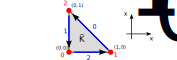
\includegraphics[width=1\linewidth]{figures/reference_triangle.pdf}
{\footnotesize reference triangle}
\end{center}
\end{frame}

%%%%%%%%%%%%%%%%%%%%%%%%%%%%%%%%%%%%%%%%%%%%%%%%%%%%%%%%%%%%%%%%%%

\begin{frame}
\frametitle{Function space}
Polynomials of degree $p$
$$
\begin{aligned}
\mathcal{V}_h &= \mathcal{P}_p(\widehat{K})\subset H^1(\widehat{K})\\
&= \Big\{q:q(x) = \sum_{\substack{s_0,s_1\\s_0+s_1\le p}} a_{s_0,s_1} x_0^{s_0}x_1^{s_1}\;\text{$\forall\;x\in \widehat{K}$ with $a_{s_0,s_1}\in\mathbb{R}$}\Big\}
\end{aligned}
$$
\textbf{Basis functions}
$$
\{\phi_\ell\}_{\ell=0}^{\nu-1}\qquad\text{with $n_{\text{dof}}=\nu = {p+2 \choose 2} = \frac{1}{2}(p+2)(p+1)$}
$$
Naive choice: monomials
$$
\{\phi_\ell\}_{\ell=0}^{\nu-1} = \{1,x_0,x_1,x_0^2,x_0x_1,x_1^2,\dots\}
$$
Better choice: \textbf{Lagrange polynomials}
\end{frame}

%%%%%%%%%%%%%%%%%%%%%%%%%%%%%%%%%%%%%%%%%%%%%%%%%%%%%%%%%%%%%%%%%%

\begin{frame}
\frametitle{Lagrange polynomials}
\textbf{One dimension}\\
Lagrange polynomial $p$ = unique polynomial of degree $m$ which passes through $m+1$ points $\{(t_k,z_k)\}_{k=0}^{m}$:
$$
p(t_k)=z_k\qquad\text{for all $k=0,1,\dots,m$}
$$
\begin{center}
\includegraphics[width=0.55\linewidth]{figures/lagrange_polynomials_1d.png}
\end{center}
\textbf{Two dimensions}\\
Choose $\nu$ points $\{\xi^{(\ell)}\}_{\ell=0}^{\nu-1}$ in $\widehat{K}$ and define $\phi_\ell(x)\in\mathcal{P}_p(K)$ such that
$$
\phi_\ell(\xi^{(k)}) = \delta_{\ell k} = \begin{cases}
    1 & \text{for $\ell=k$}\\
    0 & \text{otherwise}.
\end{cases}
$$
\end{frame}

%%%%%%%%%%%%%%%%%%%%%%%%%%%%%%%%%%%%%%%%%%%%%%%%%%%%%%%%%%%%%%%%%%

\begin{frame}
\frametitle{Lagrange polynomials}
\textbf{Nodal points}\\[-3ex]
$$
\{\xi^{(\ell)}\}_{\ell=0}^{\nu-1} = \left\{\left(\frac{\ell_0}{p},\frac{\ell_1}{p}\right) \quad \text{for $\ell_0,\ell_1\in\mathbb{N}$ with $0\le \ell_0\le \ell_1 \le p$}\right\}
$$
\begin{center}
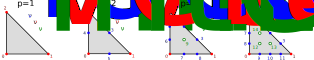
\includegraphics[width=0.9\linewidth]{figures/lagrange_nodes.pdf}
\end{center}
\textbf{Ordering of points}\\[1ex]
\begin{minipage}{0.75\linewidth}
\begin{itemize}
  \item $\nu_{\text{vertex}}=1$ point associated with each vertex \textcolor{red}{$v_0$}, \textcolor{red}{$v_1$}, \textcolor{red}{$v_2$} (in this order); 
  \item $\nu_{\text{facet}}=p-1$ points associated with each facet \textcolor{blue}{$F_0$}, \textcolor{blue}{$F_1$}, \textcolor{blue}{$F_2$} (in this order), numbered following arrows
  \item $\nu_{\text{interior}}=\frac{1}{2}(p-1)(p-2)$ points associated with interior $K^0$
\end{itemize}
\end{minipage}
\hfill
\begin{minipage}{0.225\linewidth}
  \begin{center}
  \includegraphics[width=\linewidth]{figures/reference_triangle_small.pdf}
  \end{center}
\end{minipage}
\end{frame}

%%%%%%%%%%%%%%%%%%%%%%%%%%%%%%%%%%%%%%%%%%%%%%%%%%%%%%%%%%%%%%%%%%

\begin{frame}
\frametitle{Examples}

\textbf{Linear finite element} $p=1$
$$
\begin{aligned}
\phi_0(x) &= 1-x_0-y_0\\
\phi_1(x) &= x_0\\
\phi_2(x) &= x_1
\end{aligned}
$$
$\nu_{\text{vertex}}=1$, $\nu_{\text{facet}}=\nu_{\text{interior}}=0$
\end{frame}

%%%%%%%%%%%%%%%%%%%%%%%%%%%%%%%%%%%%%%%%%%%%%%%%%%%%%%%%%%%%%%%%%%

\begin{frame}
\frametitle{Examples}
\textbf{Quadratic element} $p=2$\qquad ($\nu_{\text{interior}}=0$)\\[1ex]
\begin{minipage}{0.475\linewidth}
vertices ($\nu_{\text{vertex}}=1$)
$$
{\footnotesize
\begin{aligned}
\phi_0(x) &= (1-x_0-x_1)(1-2x_0-2x_1),\\
\phi_1(x) &= x_0(2x_0-1),\\
\phi_2(x) &= x_1(2x_1-1),
\end{aligned}
}
$$
\end{minipage}
\hfill
\begin{minipage}{0.475\linewidth}
facets ($\nu_{\text{facet}}=1$)
$$
{\footnotesize
\begin{aligned}
\phi_3(x) &= 4x_0x_1,\\
\phi_4(x) &= 4x_1(1-x_0-x_1),\\
\phi_5(x) &= 4x_0(1-x_0-x_1),
\end{aligned}}
$$
\end{minipage}
\begin{center}
\includegraphics[width=0.9\linewidth]{figures/quadratic_element.png}
\end{center}
\end{frame}

%%%%%%%%%%%%%%%%%%%%%%%%%%%%%%%%%%%%%%%%%%%%%%%%%%%%%%%%%%%%%%%%%%

\begin{frame}
\frametitle{Dual spaces}
Domain $\Omega$, space $\mathcal{V}=\mathcal{V}(\Omega)$ of real-valued functions $w:\Omega\rightarrow \mathbb{R}$\\[1ex]
\textbf{Linear functional}
$$
\lambda : \mathcal{V} \rightarrow \mathbb{R},\qquad w \mapsto \lambda(w)\in\mathbb{R}
$$
such that for all $c_1,c_2\in\mathbb{R}$, $w^{(1)}, w^{(2)} \in \mathcal{V}$
$$
\lambda(c_1 w^{(1)}+c_2 w^{(2)}) = c_1\lambda(w^{(1)})+c_2 \lambda(w^{(2)})
$$
\textbf{Dual space} $\mathcal{V}^*$ = space of all linear functionals on $\mathcal{V}$\\[2ex]
$\text{dim}(\mathcal{V})=\text{dim}(\mathcal{V}^*)$ if $\text{dim}(\mathcal{V})<\infty$
\end{frame}

%%%%%%%%%%%%%%%%%%%%%%%%%%%%%%%%%%%%%%%%%%%%%%%%%%%%%%%%%%%%%%%%%%

\begin{frame}
\frametitle{Examples}
Let $\Omega\subset \mathbb{R}^2$ and $\mathcal{V}=H^1(\Omega)$\\[2ex]
\textbf{Linear functionals} $\lambda\in\mathcal{V}^*$
\begin{itemize}
\item \textbf{point evaluation}: $\lambda(w) := w(\xi)$ for some point $\xi\in \Omega$
\item \textbf{differentiation}: $\lambda(w) := \frac{\partial w}{\partial x_0}(\xi)$ for some point $\xi\in \Omega$
\item \textbf{integration}: $\lambda(w) := \int_\Omega fw\;dx$ for some function $f \in L_2(\Omega)$
\end{itemize}
\end{frame}

%%%%%%%%%%%%%%%%%%%%%%%%%%%%%%%%%%%%%%%%%%%%%%%%%%%%%%%%%%%%%%%%%%

\begin{frame}
\frametitle{Ciarlet's definition of the finite element}
Finite element = triple $(\widehat{K},\widehat{\mathcal{V}},\mathcal{L})$
\begin{enumerate}
\item \textbf{domain} $\widehat{K}$ (= reference triangle)
\item \textbf{function space} $\widehat{\mathcal{V}}=\widehat{\mathcal{V}}(\widehat{K})$ of real-valued functions on $\widehat{K}$
\item \textbf{degrees of freedom} {\footnotesize(or \textbf{nodes})} $\mathcal{L} = \{\lambda_\ell\}_{\ell=0}^{\nu-1}$ = basis for $\widehat{\mathcal{V}}^*$
\end{enumerate}
\vspace{2ex}
$\Rightarrow$ \textbf{nodal basis} $\{\phi_\ell\}_{\ell=0}^{\nu-1}$
$$
\lambda_\ell (\phi_k) = \delta_{\ell k} \qquad\text{for all $\ell,k=0,1,\dots,\nu-1$}
$$
\end{frame}

%%%%%%%%%%%%%%%%%%%%%%%%%%%%%%%%%%%%%%%%%%%%%%%%%%%%%%%%%%%%%%%%%%

\begin{frame}
\frametitle{Examples}
\textbf{Polynomial Lagrange element}
\begin{enumerate}
\item $\widehat{K}$ the reference triangle
\item $\widehat{\mathcal{V}} = \mathcal{P}_p(\widehat{K})$ = space of bi-variate polynomials of degree $p$
\item $\mathcal{L}=\{\lambda_\ell\}_{\ell=0}^{\nu-1}$, $\lambda_\ell(w) = w(\xi^{(\ell)})$ {\footnotesize (= evaluation at nodal points $\xi^{(\ell)}$)}
\end{enumerate}
\vspace{2ex}
Alternative choice of dofs: for some point $\mathring{\xi}\in \widehat{K}$
$$
\lambda_\ell (w) = \frac{\partial^{\ell_a}w}{\partial x_0^{\ell_b} \partial x_1^{\ell_a-\ell_b}}(\mathring{\xi}) 
$$
for $0\le \ell_b \le \ell_a\le p$ and $\ell=\frac{1}{2}\ell_a(\ell_a-1) + \ell_b$
\end{frame}

%%%%%%%%%%%%%%%%%%%%%%%%%%%%%%%%%%%%%%%%%%%%%%%%%%%%%%%%%%%%%%%%%%

\begin{frame}
\frametitle{Examples}

Two-dimensional \textbf{Argyris finite element}
\begin{enumerate}
\item $\widehat{K}$ = reference triangle
\item $\widehat{\mathcal{V}} = \mathcal{P}_5(\widehat{K})$, the space of quintic bi-variate polynomials
\item 21 nodes ($\nu_{\text{vertex}}=6$, $\nu_{\text{facet}}=1$, $\nu_{\text{interior}}=0$) defined as:
\begin{itemize}
  \item $\lambda_\rho(w) = w(v_\rho)$ {\footnotesize(evaluation at each vertex $v_\rho$ $\Rightarrow$ 3 nodes)}
  \item $\lambda_{3+2\rho+a}(w) = \frac{\partial w}{\partial x_a}(v_\rho)$\\{\footnotesize(two gradient evaluations at each vertex $v_\rho$ $\Rightarrow$ 6 nodes)}
  \item $\lambda_{9+3\rho+2a+b}(w) = \frac{\partial^2 w}{\partial x_a \partial x_b}(v_\rho)$ with $0\le a\le b\le 1$\\{\footnotesize(Hessian evaluation at each vertex $v_\rho$ $\Rightarrow$ 9 nodes)}
  \item $\lambda_{18+\rho}(w) = n_\rho\cdot \nabla w(m_\rho)$\\{\footnotesize(normal derivative evaluation at the midpoints $m_\rho$ of each facet $F_\rho$ $\Rightarrow$ 3 nodes)}
\end{itemize}
\end{enumerate}
Only differs from $p=5$ polynomial element in choice of nodes
\end{frame}

%%%%%%%%%%%%%%%%%%%%%%%%%%%%%%%%%%%%%%%%%%%%%%%%%%%%%%%%%%%%%%%%%%

\begin{frame}
\frametitle{Ordering of degrees of freedom}
Node $\leftrightarrow$ topological entity of $\widehat{K}$
\begin{minipage}{0.6\linewidth}
\textbf{topological entities}
\begin{itemize}
\item \textcolor{red}{vertices $v_0$, $v_1$, $v_2$} (in this order)
\item \textcolor{blue}{facets $F_0$, $F_1$, $F_2$} (in this order)
\item interior $K^0$
\end{itemize}
\end{minipage}
\hfill
\begin{minipage}{0.3\linewidth}
  \begin{center}
  \includegraphics[width=\linewidth]{figures/reference_triangle_small.pdf}
  \end{center}
\end{minipage}\\
Recall:
\begin{itemize}
\item $\nu_{\text{vertex}}$ nodes per vertex
\item $\nu_{\text{facet}}$ nodes per facet 
\item $\nu_{\text{interior}}$ nodes in interior $K^0$
\end{itemize}
Total number of nodes (dofs)
$$
\nu = 3( \nu_{\text{vertex}}+\nu_{\text{facet}})+\nu_{\text{interior}}.
$$
\end{frame}

%%%%%%%%%%%%%%%%%%%%%%%%%%%%%%%%%%%%%%%%%%%%%%%%%%%%%%%%%%%%%%%%%%

\begin{frame}
  \frametitle{Ordering of degrees of freedom}
Arrange degrees of freedom $\{\lambda_0,\dots,\lambda_{\nu-1}\}$ in the order
$$
\underbrace{v_0 \rightarrow v_1 \rightarrow v_2}_{\text{(vertices)}}
\rightarrow \underbrace{F_0 \rightarrow F_1 \rightarrow F_2}_{\text{(facets)}}
\rightarrow \underbrace{K^0}_{\text{(interior)}}
$$
$\lambda_j^{(E_\rho)}$ = $j$-th node associated with $E_\rho\in \{v_0,v_1,v_2,F_0,F_1,F_2,K^0\}$
\begin{center}
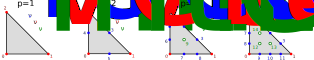
\includegraphics[width=0.8\linewidth]{figures/lagrange_nodes.pdf}
\end{center}
$$
\begin{aligned}
& \{\lambda_0^{(v_0)},\dots,\lambda_{\nu_{\text{vertex}}-1}^{(v_0)},
\lambda_0^{(v_1)},\dots,\lambda_{\nu_{\text{vertex}}-1}^{(v_1)},
\lambda_0^{(v_2)},\dots,\lambda_{\nu_{\text{vertex}}-1}^{(v_2)},\\
& \lambda_0^{(F_0)},\dots,\lambda_{\nu_{\text{facet}}-1}^{(F_0)},
\lambda_0^{(F_1)},\dots,\lambda_{\nu_{\text{facet}}-1}^{(F_1)},
\lambda_0^{(F_2)},\dots,\lambda_{\nu_{\text{facet}}-1}^{(F_2)},\\
& \lambda_0^{(K^0)},\dots,\lambda_{\nu_{\text{interior}}-1}^{(K^0)}
\}
\end{aligned}
$$
\end{frame}

%%%%%%%%%%%%%%%%%%%%%%%%%%%%%%%%%%%%%%%%%%%%%%%%%%%%%%%%%%%%%%%%%%

\begin{frame}
\frametitle{Ordering of degrees of freedom}
\textbf{Indirection map} $\mu_{\text{dof}}$: $\lambda_{\ell=\mu_{\text{dof}}(E,\rho,j)} = \lambda_j^{(E_\rho)}$
$$
\mu_{\text{dof}}(E,\rho,j) = \begin{cases}
\rho\cdot \nu_{\text{vertex}} + j & \text{if $E_\rho$ is the $\rho$-th vertex}\\
3\nu_{\text{vertex}} + \rho\cdot \nu_{\text{facet}} + j & \text{if $E_\rho$ is the $\rho$-th facet}\\
3(\nu_{\text{vertex}} + \nu_{\text{facet}}) + j & \text{if $E$ is the interior}
\end{cases}
$$
Example: \textbf{quartic Lagrange element} ($p=4$)\\[2ex]
\begin{minipage}{0.3\linewidth}
$$
\begin{aligned}
\mu_{\text{dof}}(v,1,0) &= 1\\
\mu_{\text{dof}}(F,0,2) &= 5\\
\mu_{\text{dof}}(K^0,0,2) &= 14
\end{aligned}
$$
\end{minipage}
\hfill
\begin{minipage}{0.3\linewidth}
  \begin{center}
  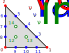
\includegraphics[width=\linewidth]{figures/lagrange_nodes_quintic.pdf}
  \end{center}
\end{minipage}
\hfill
\begin{minipage}{0.3\linewidth}
  \begin{center}
  \includegraphics[width=\linewidth]{figures/reference_triangle_small.pdf}
  \end{center}
\end{minipage}
\end{frame}

%%%%%%%%%%%%%%%%%%%%%%%%%%%%%%%%%%%%%%%%%%%%%%%%%%%%%%%%%%%%%%%%%%

\begin{frame}
\frametitle{Vandermonde matrix}
\textbf{Nodal basis functions} $\{\phi_\ell(x)\}_{\ell=0}^{\nu-1}$\\
Start with basis of $\widehat{\mathcal{V}}$:
$$
\{\theta_m(x)\}_{m=0}^{\nu-1}=\{1,x_0,x_1,x_0^2,x_0x_1,x_1^2,\dots\}
$$
and expand
$$
\phi_k(x) = \sum_{m=0}^{\nu-1} c_m^{(k)} \theta_m(x)\qquad\text{for coefficients $c_m^{(k)}$}
$$
Definition of nodal basis
$$
\delta_{\ell k} = \lambda_\ell(\phi_k) = \sum_{m=0}^{\nu-1} \underbrace{c_m^{(k)}}_{C_{mk}} \underbrace{\lambda_\ell(\theta_m)}_{V_{\ell m}}
$$
\end{frame}

%%%%%%%%%%%%%%%%%%%%%%%%%%%%%%%%%%%%%%%%%%%%%%%%%%%%%%%%%%%%%%%%%%

\begin{frame}
\frametitle{Vandermonde matrix}

Define $\nu\times\nu$ matrices $V$, $C$ with $V_{\ell m} := \lambda_\ell(\theta_m)$ and $C_{mk}:=c_m^{(k)}$

$$
\delta_{\ell k} =  \sum_{m=0}^{\nu-1} c_m^{(k)} \lambda_\ell(\theta_m)
\quad \Leftrightarrow \quad
VC = \mathbb{I}\quad \Leftrightarrow \quad C = V^{-1}
$$
Lagrange element $\lambda_\ell(w) = w(\xi^{(\ell)})$ $\Rightarrow$ $V_{\ell m} = \lambda_{\ell}(\theta_m) = \theta_m(\xi^{(\ell)})$\\[1ex]
\textbf{Vandermonde matrix}
$$
\setlength\arraycolsep{2pt}
{\footnotesize%
V = V(\{\xi^{(\ell)}\}_{\ell=0}^{\nu-1}) = \begin{pmatrix}
1 & \xi^{(0)}_0 & \xi^{(0)}_1  & (\xi^{(0)}_0)^2 & \xi^{(0)}_0 \xi^{(0)}_1 & (\xi^{(0)}_1)^2 & \dots \\[1ex]
1 & \xi^{(1)}_0 & \xi^{(1)}_1 & (\xi^{(1)}_0)^2 & \xi^{(1)}_0 \xi^{(1)}_1 & (\xi^{(1)}_1)^2 & \dots \\[1ex]
1 & \xi^{(2)}_0 & \xi^{(2)}_1 & (\xi^{(2)}_0)^2 & \xi^{(2)}_0 \xi^{(2)}_1 & (\xi^{(2)}_1)^2 & \dots \\[1ex]
\vdots & \vdots & \vdots & \vdots & \vdots & \vdots & \ddots\\
1 & \xi^{(\nu-1)}_0 & \xi^{(\nu-1)}_1 & (\xi^{(\nu-1)}_0)^2 & \xi^{(\nu-1)}_0 \xi^{(\nu-1)}_1 & (\xi^{(\nu-1)}_1)^2 & \dots
\end{pmatrix}}
$$
\textbf{Nodal basis functions}
$$
\phi_k(x) = \sum_{m=0}^{\nu-1} C_{mk} \theta_m(x)\qquad\text{with $C_{mk} = (V^{-1})_{mk}$}
$$
\end{frame}

%%%%%%%%%%%%%%%%%%%%%%%%%%%%%%%%%%%%%%%%%%%%%%%%%%%%%%%%%%%%%%%%%%

\begin{frame}
\frametitle{Evaluation of basis functions}
Consider any $n$ points
$$
\boldsymbol{\zeta}:=\{\zeta^{(r)}\}_{r=0}^{n-1}\qquad\text{with $\zeta^{(r)}\in\widehat{K}$}
$$
Define
\begin{itemize}
\item $n\times\nu$ matrix $V(\boldsymbol{\zeta})$
$$
V_{rm}(\boldsymbol{\zeta}) := \theta_m(\zeta^{(r)})
$$
\item Rank 3 tensor $V^{\partial}(\boldsymbol{\zeta})$ of shape $[n,\nu,2]$
$$
V^{\partial}_{rma}(\boldsymbol{\zeta}):=\frac{\partial \theta_m}{\partial x_a}(\zeta^{(r)}).
$$
\end{itemize}
\end{frame}

%%%%%%%%%%%%%%%%%%%%%%%%%%%%%%%%%%%%%%%%%%%%%%%%%%%%%%%%%%%%%%%%%%

\begin{frame}
\frametitle{Tabulation of basis functions}
\textbf{Evaluation of nodal basis functions}: $n\times \nu$ matrix $T(\vec{\zeta})$
$$
T_{r\ell}(\boldsymbol{\zeta}) := \phi_\ell(\zeta^{(r)}) = \sum_{m=0}^{\nu-1} c_m^{(\ell)} \theta_m(\zeta^{(r)}) = \sum_{m=0}^{\nu-1}V_{rm}(\boldsymbol{\zeta})C_{m\ell}
$$
$$
T(\boldsymbol{\zeta}) = V(\boldsymbol{\zeta}) C\qquad\text{with $C=V^{-1}$}
$$
\textbf{Evaluation of derivatives}: rank 3 tensor $T^\partial(\vec{\zeta})$ of shape $[n,\nu,2]$
$$
\begin{aligned}
T^\partial_{r\ell a}(\boldsymbol{\zeta}) &:= \frac{\partial \phi_\ell}{\partial x_a}(\zeta^{(r)}) 
 = \sum_{m=0}^{\nu-1} c_m^{(\ell)} \frac{\partial \theta_m}{\partial x_a}(\zeta^{(r)}) \\
 &= \sum_{m=0}^{\nu-1} V^\partial_{rma}(\boldsymbol{\zeta})C_{m\ell}
 \end{aligned}
$$
\end{frame}


%%%%%%%%%%%%%%%%%%%%%%%%%%%%%%%%%%%%%%%%%%%%%%%%%%%%%%%%%%%%%%%%%%

\begin{frame}
\frametitle{Implementation}
Ciarlet's definition of finite element\\[1ex]
$\Rightarrow$
\textbf{Abstract base class} \lstinline{FiniteElement}
\begin{itemize}
\item \# nodes associated with each topological entity
\begin{itemize}
  \item abstract properties \lstinline{ndof_per_vertex}, \lstinline{ndof_per_facet}, \lstinline{ndof_per_interior} for $\nu_{\text{vertex}}$, $\nu_{\text{facet}}$ and $\nu_{\text{interior}}$. 
  \item property \lstinline{ndof}: $\nu =3(\nu_{\text{vertex}}+\nu_{\text{facet}})+\nu_{\text{interior}}$
\end{itemize}
\item Tabulate evaluation of dofs for given $\hat{f}$ $\Rightarrow$ abstract method \lstinline{tabulate_dofs(fhat)} returns $(\lambda_0(\hat{f}),\lambda_1(\hat{f}),\dots,\lambda_{\nu-1}(\hat{f}))^\top$
\item Tabulate basis functions for $\boldsymbol{\zeta}=\{\zeta^{(r)}\}_{r=0}^{n-1}$ $\Rightarrow$ abstract method \lstinline{tabulate(zeta)} returns $n\times\nu$ matrix $T$ with $T_{r\ell}=\phi_\ell(\zeta^{(r)})$ 
\item Tabulate gradients of basis functions for $\boldsymbol{\zeta}=\{\zeta^{(r)}\}_{r=0}^{n-1}$ $\Rightarrow$ abstract method \lstinline{tabulate_gradient(zeta)} returns rank 3 tensor $T^\partial$ of shape $n\times\nu\times 2$ with $T^\partial_{r\ell a}=\frac{\partial\phi_\ell}{\partial x_a}(\zeta^{(r)})$. 
\item dof-map $\mu_{\text{dof}}(E,\rho,j)$ and its inverse\\$\Rightarrow$ \lstinline{dofmap(entity_type,rho,j)}, \lstinline{inverse_dofmap(ell)}
\end{itemize}
\end{frame}

%%%%%%%%%%%%%%%%%%%%%%%%%%%%%%%%%%%%%%%%%%%%%%%%%%%%%%%%%%%%%%%%%%

\begin{frame}
\frametitle{Concrete implementations}
\textbf{Subclassing} the \lstinline{FiniteElement} base class\\
$\Rightarrow$ Provide concrete implementations of:
\begin{itemize}
\item \# dofs associated with topological entities:\\\lstinline{ndof_per_vertex}, \lstinline{ndof_per_facet} and \lstinline{ndof_per_interior}
\item Evalute dofs for given function $\widehat{f}$: \lstinline{tabulate_dofs(fhat)} 
\item Tabulate basis functions: \lstinline{tabulate(zeta)}
\item Tabulate gradients of basis functions: \lstinline{tabulate_gradient(zeta)}
\end{itemize}
\end{frame}

%%%%%%%%%%%%%%%%%%%%%%%%%%%%%%%%%%%%%%%%%%%%%%%%%%%%%%%%%%%%%%%%%%

\begin{frame}[fragile]
\frametitle{Concrete implementations}
Available finite elements
\begin{itemize}
\item Bi-linear element $(p=1)$: \lstinline{LinearElement}
\item Cubic linear element $(p=3)$: \lstinline{CubicElement} (= exercise)
\item General polynomial element: \lstinline{PolynomialElement} (will be made available later)
\end{itemize}
\vspace{2ex}
Import as
\begin{lstlisting}
from fem.linearelement import LinearElement
from fem.polynomialelement import PolynomialElement
\end{lstlisting}
\end{frame}

%%%%%%%%%%%%%%%%%%%%%%%%%%%%%%%%%%%%%%%%%%%%%%%%%%%%%%%%%%%%%%%%%%

\begin{frame}
\frametitle{Numerical quadrature}
The weak form of PDE requires \textbf{integration} over domain $\Omega$
$$
a(u,v) = \int_\Omega \left(\kappa \nabla u \cdot \nabla  v + \omega\; u v\right)\;dx
$$
\textbf{Numerical integration in 1d}
$$
\int_{-1}^{+1} f(z)\;dz \approx \sum_{q=0}^{n_q-1} \widetilde{w}_q f(\widetilde{\zeta}^{(q)})
$$
\textbf{Qudrature\footnote{often called ``cubature'' in more than one dimension} rule} $\mathcal{Q}=\{(\widetilde{\zeta}^{(q)},\widetilde{w}_q)\}_{q=0}^{n_q-1}$
\begin{itemize}
\item points $\widetilde{\zeta}^{(q)}$, $q=0,1,2,\dots,n_q-1$
\item corresponding weights $\widetilde{w}_q$
\end{itemize}
\end{frame}

%%%%%%%%%%%%%%%%%%%%%%%%%%%%%%%%%%%%%%%%%%%%%%%%%%%%%%%%%%%%%%%%%%

\begin{frame}[fragile]
\frametitle{Numerical quadrature}
\textbf{Gauss-Legendre quadrature} $\mathcal{Q}^{(\text{GL})}_{n_q}$
\begin{itemize}
 \item points $\widetilde{\zeta}^{(q)}$ = roots of the Legendre polynomial $P_{n_q}$
 \item weights $\widetilde{w}_q = \frac{2}{(1-(\widetilde{\zeta}^{(q)})^2)(P_{n_q}'(\widetilde{\zeta}^{(q)}))^2}$
\end{itemize}

\begin{lstlisting}
points, weights = numpy.polynomial.legendre.leggauss(n_q)
\end{lstlisting}
\textbf{Exact} for polynomials of degree $2n_q-1$:

$$
\int_{-1}^{+1} p(z)\;dz = \sum_{q=0}^{n_q-1} \widetilde{w}_q p(\widetilde{\zeta}^{(q)})\qquad\text{for $p\in\mathcal{P}_{2n_q-1}$}
$$
\textbf{degree of precision} (dop)
$$
\text{dop}(\mathcal{Q}^{(\text{GL})}_{n_q}) = 2n_q-1
$$
\end{frame}

%%%%%%%%%%%%%%%%%%%%%%%%%%%%%%%%%%%%%%%%%%%%%%%%%%%%%%%%%%%%%%%%%%

\begin{frame}[fragile]
\frametitle{Numerical quadrature}
\textbf{Lowest order Gauss-Legendre} quadrature rules
\begin{center}
  \renewcommand{\arraystretch}{2.5}
  \begin{tabular}{cccc}
    \hline
    \# points $n_q$ & points $\widetilde{\zeta}^{(q)}$ & weights $\widetilde{w}_q$ & $\text{dop}(\mathcal{Q}^{(\text{GL})}_{n_q})$\\
    \hline\hline
 1   & $0$ & $2$ & $1$\\
 2   & $-\sqrt{\frac{1}{3}}, +\sqrt{\frac{1}{3}}$ & $1$ & $3$\\
 3   & $-\sqrt{\frac{3}{5}},0,+\sqrt{\frac{3}{5}}$ & $\frac{5}{9},\frac{8}{9},\frac{5}{9}$ & $5$\\
 \hline
  \end{tabular}
\end{center}
\end{frame}

%%%%%%%%%%%%%%%%%%%%%%%%%%%%%%%%%%%%%%%%%%%%%%%%%%%%%%%%%%%%%%%%%%

\begin{frame}[fragile]
\frametitle{Integration along a line}
\textbf{Integrate function along a straight line} $\mathcal{C}\subset \mathbb{R}^2$ connecting two points $a,b\in \mathbb{R}^2$\\[1ex]
\begin{minipage}{0.6\linewidth}
Parametrisation $\gamma: [-1,1] \rightarrow \mathbb{R}^2$ 
\end{minipage}
\hfill
\begin{minipage}{0.25\linewidth}
  \begin{center}
  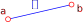
\includegraphics[width=\linewidth]{figures/straight_line.pdf}
  \end{center}
\end{minipage}
$$
\gamma(z) = \frac{1-z}{2}a+\frac{1+z}{2}b\qquad\text{\footnotesize note: $\gamma(-1)=a$, $\gamma(1)=b$}
$$
$$
\begin{aligned}
\Rightarrow\quad \int_{\mathcal{C}} f(x)\;ds &= \frac{\|b-a\|}{2} \int_{-1}^{+1} f(\gamma(z))\;dz \approx \sum_{q=0}^{n_q-1} w_{\mathcal{C},q} f(\zeta_{\mathcal{C}}^{(q)})
\end{aligned}
$$

\textbf{GL quadrature rule on $\mathcal{C}$}: $\mathcal{Q}^{(\text{GL},\mathcal{C})}_{n_q}=\{(\zeta^{(q)}_{\mathcal{C}},w_{\mathcal{C},q})\}_{q=0}^{n_q-1}$
$$
\zeta_{\mathcal{C}}^{(q)} = \gamma(\widetilde{\zeta}^{(q)}) = \frac{1}{2}(1-\widetilde{\zeta}^{(q)})a + \frac{1}{2}(1+\widetilde{\zeta}^{(q)})b,\qquad
w_{\mathcal{C},q} = \frac{\|b-a\|}{2} \widetilde{w}_q
$$
$$
\text{dop}(\mathcal{Q}^{(\text{GL},\mathcal{C})}_{n_q}) = \text{dop}(\mathcal{Q}^{(\text{GL})}_{n_q}) = 2n_q-1.
$$
\end{frame}

%%%%%%%%%%%%%%%%%%%%%%%%%%%%%%%%%%%%%%%%%%%%%%%%%%%%%%%%%%%%%%%%%%

\begin{frame}[fragile]
\frametitle{Two-dimensional quadrature for the reference triangle}
Duffy transform $\tau$: $S=[-1,+1]\times [-1,+1]\mapsto \widehat{K} = \tau(S)$
$$
\begin{aligned}
\tau(\widetilde{x}) = \begin{pmatrix}\frac{1}{2}(1+\widetilde{x}_0)\\[1ex]\frac{1}{4}(1-\widetilde{x}_0)(1+\widetilde{x}_1)\end{pmatrix} \in \widehat{K}\qquad\text{for $\widetilde{x}=(\widetilde{x}_0,\widetilde{x}_1)\in S$}
\end{aligned}
$$
\begin{center}
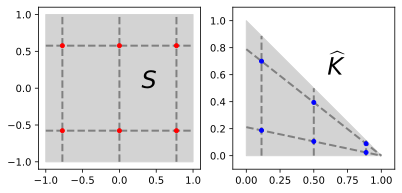
\includegraphics[width=0.5\linewidth]{figures/quadrature.pdf}
\end{center}
\textbf{Quadrature on} $\boldsymbol{S}=[-1,+1]\times[-1,+1]$ $\Rightarrow$ product of 1d rules\\$\mathcal{Q}_{n_q+1}^{(\text{GL})} = \{(\widetilde{\zeta}^{(q_0)}_0,\widetilde{w}_{0,q_1})\}_{q_0=0}^{n_q}$, $\mathcal{Q}_{n_q}^{(\text{GL})} =\{(\widetilde{\zeta}^{(q_1)}_1,\widetilde{w}_{1,q_1})\}_{q_1=0}^{n_q-1}$\\[1ex]
2d quadrature rule $\mathcal{Q}_{n_q}^{(\text{GL},S)}=\{(\widetilde{\zeta}^{(q)},\widetilde{w}_q)\}_{q=0}^{N_q-1}$, $N_q = n_q(n_q+1)$
$$
\widetilde{\zeta}^{(q)} = \begin{pmatrix}\widetilde{\zeta}^{(q_0)}_0\\[1ex]\widetilde{\zeta}^{(q_1)}_1\end{pmatrix}\in\mathbb{R}^2,\quad \widetilde{w}_i = \widetilde{w}_{0,q_0}\cdot \widetilde{w}_{1,q_1} \qquad \text{$q=n_q q_0+q_1$}.
$$
\end{frame}

%%%%%%%%%%%%%%%%%%%%%%%%%%%%%%%%%%%%%%%%%%%%%%%%%%%%%%%%%%%%%%%%%%

\begin{frame}[fragile]
\frametitle{Two-dimensional quadrature for the reference triangle}
\textbf{Integration over $\boldsymbol{\widehat{K}}$}\\
Duffy transform $\tau$ $\Rightarrow$ quadrature rule on $\widehat{K}$ $\mathcal{Q}_{n_q}^{(\text{GL},\widehat{K})} = \{(\zeta^{(q)},w_q)\}_{q=0}^{N_q-1} = \tau(\mathcal{Q}^{(S)}_{n_q})$ over $\widehat{K}$:

$$
\begin{aligned}
\zeta^{(q)} &= \tau(\widetilde{\zeta}^{(q)}) = \begin{pmatrix}(\frac{1}{2}(1+\widetilde{\zeta}^{(q_0)}_0)\\[1ex]\frac{1}{4}(1-\widetilde{\zeta}^{(q_0)}_0)(1+\widetilde{\zeta}^{(q_1)}_1)\end{pmatrix}\qquad \text{where $q=n_qq_0+q_1$}\\
w_q &= \widetilde{w}_q \left|\det\left(\frac{\partial \tau}{\partial \widetilde{x}}\right)\right|_{\widetilde{x}=\widetilde{\zeta}^{(q)}}= \frac{1}{8}\widetilde{w}_{0,q_0}\widetilde{w}_{1,q_1}(1-\widetilde{\zeta}^{(q_0)}_0)
\end{aligned}
$$
\begin{center}
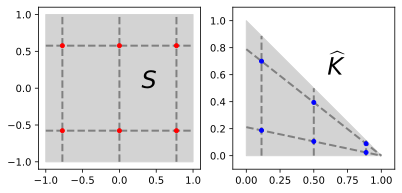
\includegraphics[width=0.5\linewidth]{figures/quadrature.pdf}
\end{center}
$$
\text{dop}(\mathcal{Q}^{(\text{GL},\widehat{K})}_{n_q}) = \text{dop}(\mathcal{Q}^{(\text{GL})}_{n_q}) = 2n_q-1.
$$
\end{frame}

%%%%%%%%%%%%%%%%%%%%%%%%%%%%%%%%%%%%%%%%%%%%%%%%%%%%%%%%%%%%%%%%%%

\begin{frame}[fragile]
\frametitle{Implementation in Python}
\textbf{Abstract base class} \lstinline{Quadrature}
\begin{itemize}
\item Points $\{\zeta^{(q)}\}_{q=0}^{n_q-1}$ $\Rightarrow$ array \lstinline{nodes} of shape $n_q\times 2$
\item Weights $\{w_q\}_{q=0}^{n_q-1}$ $\Rightarrow$ array \lstinline{weights} of length $n_q$
\item degree of precision $\Rightarrow$ property \lstinline{degree_of_precision}
\end{itemize}
\vspace{2ex}
Concrete implementations in \textbf{subclasses}
\begin{itemize}
  \item Quadrature rule $\mathcal{Q}^{(\text{GL},\mathcal{C})}_{n_q}$ over line segment $\mathcal{C}$: \lstinline{GaussLegendreQuadratureLineSegment(v_a, v_b, npoints)}
  \begin{itemize}
    \item \lstinline{v_a} start point $a$
    \item \lstinline{v_b} end point $b$
    \item \lstinline{npoints} number of points $n_q$
  \end{itemize}
  \item Quadrature rule $\mathcal{Q}^{(\text{GL},\widehat{K})}_{n_q}$ over the reference triangle $\widehat{K}$: \lstinline{GaussLegendreQuadratureReferenceTriangle(npoints)}
\end{itemize}
\end{frame}

%%%%%%%%%%%%%%%%%%%%%%%%%%%%%%%%%%%%%%%%%%%%%%%%%%%%%%%%%%%%%%%%%%

\section{Local assembly}

%%%%%%%%%%%%%%%%%%%%%%%%%%%%%%%%%%%%%%%%%%%%%%%%%%%%%%%%%%%%%%%%%%

\begin{frame}
  \tableofcontents[currentsection]
\end{frame}

%%%%%%%%%%%%%%%%%%%%%%%%%%%%%%%%%%%%%%%%%%%%%%%%%%%%%%%%%%%%%%%%%%

\begin{frame}
\frametitle{Finite element method on triangle}
Putting it all together\\[2ex]
\textbf{Solve}
$$
\begin{aligned}
-\nabla\cdot(\kappa \cdot u) + \omega u &= f\qquad\text{in $\Omega=\widehat{K}$}\\
\kappa\; n\cdot \nabla u&=g \qquad\text{on $\partial\Omega$}
\end{aligned}
$$
\begin{itemize}
\item assemble stiffness matrix $A^{(h)}$
$$
A^{(h)}_{\ell k} = a(\phi_k,\phi_\ell) = \int_{\widehat{K}} \Big(\kappa \nabla \phi_k(x) \cdot\nabla\phi_\ell(x) + \omega\; \phi_k(x) \phi_\ell(x)\Big)\;dx
$$
\item assemble right-hand side vector $\boldsymbol{b}^{(h)}$
$$
b^{(h)}_\ell = b(\phi_\ell) = \int_{\widehat{K}} f(x)\phi_\ell(x)\;dx + \int_{\partial \widehat{K}} g(x)\phi_\ell(x)\;dx
$$
\end{itemize}
\end{frame}

%%%%%%%%%%%%%%%%%%%%%%%%%%%%%%%%%%%%%%%%%%%%%%%%%%%%%%%%%%%%%%%%%%

\begin{frame}
\frametitle{Stiffness matrix}
\textbf{Entries of stiffness matrix $\boldsymbol{A^{(h)}}$} (in $d=2$ dimensions)
$$
\begin{aligned}
A^{(h)}_{\ell k}  &= \int_{\widehat{K}} \Big(\kappa \nabla \phi_k(x) \cdot\nabla\phi_\ell(x) + \omega\; \phi_k(x) \phi_\ell(x)\Big)\;dx\\
&= \int_{\widehat{K}} \left(\kappa \sum_{a=0}^{d-1}\frac{\partial\phi_k}{\partial x_a}(x) \frac{\partial\phi_\ell}{\partial x_a}(x) + \omega\; \phi_k(x) \phi_\ell(x)\right)\;dx\\
&\approx 
\sum_{q=0}^{N_q-1} w_q\left(\kappa \sum_{a=0}^{d-1}\frac{\partial\phi_k}{\partial x_a}(\zeta^{(q)}) \frac{\partial\phi_\ell}{\partial x_a}(\zeta^{(q)}) + \omega\; \phi_k(\zeta^{(q)}) \phi_\ell(\zeta^{(q)})\right)\\
&= \kappa \sum_{q=0}^{N_q-1}\sum_{a=0}^{d-1} w_q  T^\partial_{qk a} (\boldsymbol{\zeta})T^\partial_{q\ell a} (\boldsymbol{\zeta})
+\omega \sum_{q=0}^{N_q-1} w_qT_{qk}(\boldsymbol{\zeta})T_{q\ell}(\boldsymbol{\zeta})
\end{aligned}
$$
\begin{itemize}
  \item Lagrange element of degree $p$, basis functions $\{\phi_\ell\}_{\ell=0}^{\nu-1}$
  \item Quadrature $\mathcal{Q}_{p+1}^{(\text{GL},\widehat{K})}=\{w_q,\zeta^{(q)}\}_{q=0}^{N_q-1}$ with $\text{dop}=2p+1$
  \item Tabulation matrices $T$, $T^\partial$ of $\phi$, $\nabla\phi$
\end{itemize}
\end{frame}

%%%%%%%%%%%%%%%%%%%%%%%%%%%%%%%%%%%%%%%%%%%%%%%%%%%%%%%%%%%%%%%%%%

\begin{frame}
\frametitle{Right-hand side vector}
\textbf{Entries of right-hand side vector $\boldsymbol{b^{(h)}}$}
$$
\begin{aligned}
b^{(h)}_\ell  &= \int_{\widehat{K}} f(x)\phi_\ell(x)\;dx + \int_{\partial \widehat{K}} g(x)\phi_\ell(x)\;dx\\
&\approx \sum_{q=0}^{N_q-1} w_q f(\zeta^{(q)}) \phi_\ell(\zeta^{(q)}) + \sum_{\text{facets}\;F_\rho} \sum_{q=0}^{n_q-1 }w_{F_\rho,q} g(\zeta_{F_\rho}^{(q)})\phi_\ell(\zeta_{F_\rho}^{(q)}) \\
&= \sum_{q=0}^{N_q-1} w_q f_q(\boldsymbol{\zeta}) T_{q\ell}(\boldsymbol{\zeta}) + \sum_{\text{facets}\;F_\rho} \sum_{q=0}^{n_q-1 }w_{F_\rho,q} g_{q}(\boldsymbol{\zeta}_{F_\rho})T_{q\ell}(\boldsymbol{\zeta}_{F_\rho})
\end{aligned}
$$
\begin{itemize}
  \item Function evaluation at quadrature points:\\$f_q(\boldsymbol{\zeta}):=f(\zeta^{(q)})$, $g_{q}(\boldsymbol{\zeta}_{F_\rho}) := g(\zeta_{F_\rho}^{(q)})$
  \item Quadrature rule on facet $F_\rho$: $\mathcal{Q}_{p+1}^{(\text{GL},F_\rho)} = \{w_{F_\rho,q},\zeta^{(q)}_{F_\rho}\}_{q=0}^{p}$
\end{itemize}
\end{frame}

%%%%%%%%%%%%%%%%%%%%%%%%%%%%%%%%%%%%%%%%%%%%%%%%%%%%%%%%%%%%%%%%%%

\begin{frame}
\frametitle{Error}
 \textbf{Difference between exact and numerical solution}
$$
e_h(x) = u(x)-u_h(x) = u(x) - \sum_{\ell=0}^{\nu-1} u^{(h)}_\ell \phi_\ell(x)\qquad\text{for all $x\in\widehat{K}$}
$$
Square of the \textbf{$\boldsymbol{L_2}$ error norm}
$$
\begin{aligned}
\|e_h\|_{L_2(\widehat{K})}^2 &= \int_{\widehat{K}} \Big(u(x) - \sum_{j=0}^{\nu-1} u^{(h)}_\ell \phi_\ell(x)\Big)^2\;dx\\
&\approx 
\sum_{q=0} ^{N_q-1} w_q \Big(u(\zeta^{(q)}) - \sum_{\ell=0}^{\nu-1} u^{(h)}_\ell \phi_\ell(\zeta^{(q)})\Big)^2 = \sum_{q=0} ^{N_q-1} w_q e_q^2
\end{aligned}
$$
\begin{itemize}
\item Quadrature rule $\mathcal{Q}_{n_q}^{(\widehat{K})}=\{w_q,\zeta^{(q)}\}_{q=0}^{N_q-1}$
\item Error at quadrature points $e_q = u(\zeta^{(q)}) - \sum_{\ell=0}^{\nu-1} u^{(h)}_\ell T_{q\ell}$
\end{itemize}
\end{frame}

%%%%%%%%%%%%%%%%%%%%%%%%%%%%%%%%%%%%%%%%%%%%%%%%%%%%%%%%%%%%%%%%%%

\begin{frame}
\frametitle{Numerical experiment}
\textbf{Method of manufactured solutions}\\
Assume that exact solution is
$$
u(x) = u_{\text{exact}}(x) = \exp\left[-\frac{1}{2\sigma^2}(x-x_0)^2\right]
$$
$\Rightarrow$ pick $f$, $g$ to satisfy  $-\nabla\cdot(\kappa \cdot u) + \omega u = f$, $\kappa\; n\cdot \nabla u=g$

$$
\begin{aligned}
f(x) &= \left(\left(2\frac{\kappa}{\sigma^2}+\omega\right)-\frac{\kappa}{\sigma^4}(x-x_0)^2\right) u_{\text{exact}}(x)
\\
g(x) &= -\frac{\kappa}{\sigma^2}n\cdot(x-x_0)u_{\text{exact}}(x)
\end{aligned}
$$
\begin{minipage}{0.7\linewidth}
\textbf{Solution procedure}
\begin{itemize}
\item Assemble $A^{(h)}$ and $\boldsymbol{b}^{(h)}$
\item Solve linear system $A^{(h)}\boldsymbol{u}^{(h)}=\boldsymbol{b}^{(h)}$
\item Compute $L_2$ error norm $\|e_h\|_{L_2(\widehat{K})}$
\end{itemize}
\end{minipage}
\hfill
\begin{minipage}{0.25\linewidth}
  \begin{center}
    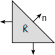
\includegraphics[width=\linewidth]{figures/reference_triangle_normals.pdf}
  \end{center}
\end{minipage}\\
\end{frame}

%%%%%%%%%%%%%%%%%%%%%%%%%%%%%%%%%%%%%%%%%%%%%%%%%%%%%%%%%%%%%%%%%%

\begin{frame}
\frametitle{Numerical experiment {\footnotesize$\kappa = 0.9$, $\omega = 0.4$, $\sigma = 0.5$, $x_0 = (0.6, 0.25)$}}
\begin{center}
  \begin{minipage}{0.8\linewidth}
    \includegraphics[width=\linewidth]{figures/triangle_solution_01.png}
  \end{minipage}
  \hfill
  \begin{minipage}{0.15\linewidth}
  $p=1$
  \end{minipage}\\
  \begin{minipage}{0.8\linewidth}
    \includegraphics[width=\linewidth]{figures/triangle_solution_03.png}
  \end{minipage}
  \hfill
  \begin{minipage}{0.15\linewidth}
  $p=3$
  \end{minipage}
\end{center}
\end{frame}

%%%%%%%%%%%%%%%%%%%%%%%%%%%%%%%%%%%%%%%%%%%%%%%%%%%%%%%%%%%%%%%%%%

\section{Error analysis}

%%%%%%%%%%%%%%%%%%%%%%%%%%%%%%%%%%%%%%%%%%%%%%%%%%%%%%%%%%%%%%%%%%

\begin{frame}
  \tableofcontents[currentsection]
\end{frame}

%%%%%%%%%%%%%%%%%%%%%%%%%%%%%%%%%%%%%%%%%%%%%%%%%%%%%%%%%%%%%%%%%%

\begin{frame}
\frametitle{Error analysis}

\textbf{Sources of error}

\begin{itemize}
\item \textcolor{blue}{Modelling error:} equations provide approximate description of physical phenomenon
\item \textcolor{blue}{Discretisation error:} for finite elements
  $$\|e_h\|_{L_2(\Omega)} \le Ch^\mu$$
  \begin{itemize}
    \item increase degree $p$
    \item decrease grid spacing $h$
  \end{itemize}
\item \textcolor{blue}{Rounding error:} approximate arithmetic on $\mathbb{R}$
\end{itemize}
\end{frame}

%%%%%%%%%%%%%%%%%%%%%%%%%%%%%%%%%%%%%%%%%%%%%%%%%%%%%%%%%%%%%%%%%%

\begin{frame}
\frametitle{Error analysis}
\textbf{Results from numerical experiment}\\
{\footnotesize$\kappa = 0.9$, $\omega = 0.4$, $\sigma = 0.5$, $x_0 = (0.6, 0.25)$}
\begin{center}
\includegraphics[width=0.8\linewidth]{figures/error_reference_triangle.png}
\end{center}
\end{frame}

%%%%%%%%%%%%%%%%%%%%%%%%%%%%%%%%%%%%%%%%%%%%%%%%%%%%%%%%%%%%%%%%%%

\begin{frame}
\frametitle{Floating point numbers}
Representation of real numbers on a computer\\
\textbf{Floating point number system}
\begin{itemize}
\item base $1<\beta\in\mathbb{N}$
\item precision $0<p\in\mathbb{N}$
\item range of exponents defined by $L,U\in\mathbb{Z}$ with $L<0\le U$
\end{itemize}
$\mathbb{F}$ = all numbers $x$ of form
$$
x = \pm \underbrace{\left(d_0 + d_1\beta^{-1} + d_2\beta^{-1} + \dots+d_{p-1}\beta^{1-p}\right)}_{\text{mantissa}}\cdot\beta^E
$$
with $d_i\in \{0,1,2,\dots,\beta-1\}$, exponent $E$ with $L\le E\le U$\\[1ex]

$\mathbb{F}$ normalised $\Leftrightarrow$ $d_0>0$ $\Rightarrow$ numbers in $\mathbb{F}$ unique.

\end{frame}

%%%%%%%%%%%%%%%%%%%%%%%%%%%%%%%%%%%%%%%%%%%%%%%%%%%%%%%%%%%%%%%%%%

\begin{frame}
\frametitle{Floating point numbers}
\textbf{Example}
$$
234.7 = \left(2+3\cdot 10^{-1}+4\cdot 10^{-2} +7\cdot 10^{-3}\right)\cdot 10^2
$$
in precision 4, base 10 arithmetic\\[2ex]
Approximation
$$
234.7 \approx \left(2+3\cdot 10^{-1}+5\cdot 10^{-2}\right)\cdot 10^2 = 235
$$
in precision 3, base 10 arithmetic

\end{frame}

%%%%%%%%%%%%%%%%%%%%%%%%%%%%%%%%%%%%%%%%%%%%%%%%%%%%%%%%%%%%%%%%%%

\begin{frame}
\frametitle{Range of representable numbers}
Floating point system $\mathbb{F}$
$$
x = \pm \left(d_0 + d_1\beta^{-1} + d_2\beta^{-1} + \dots+d_{p-1}\beta^{1-p}\right)\cdot\beta^E
$$
\textbf{Underflow threshold:}\\
Smallest positive normalised number {\footnotesize($d_0=1$, $d_i=0$ for $i>0$, $E=L$)}
$$
1\cdot \beta^L
$$
\textbf{Overflow threshold:}\\
Largest positive normalised number {\footnotesize ($d_i=\beta-1$ for $i\ge 0$, $E=U$)}
$$
\begin{aligned}
(\beta-1)\left(1+\beta^{-1}+\beta^{-2}+\dots+\beta^{1-p}\right)\cdot \beta^U &= (1-\beta^{-p})\beta^{U+1}
\end{aligned}
$$
\end{frame}

%%%%%%%%%%%%%%%%%%%%%%%%%%%%%%%%%%%%%%%%%%%%%%%%%%%%%%%%%%%%%%%%%%

\begin{frame}
\frametitle{Rounding}
$\mathbb{F}$ \textbf{not closed} under arithmetic operations:
$$
x,y\in\mathbb{F}\nRightarrow x+y\in\mathbb{F}
$$
Approximate (e.g. rounding)
$$
x+y = z \in\mathbb{R} \mapsto \tilde{z} := \mathcal{R}_{\mathbb{F}}(z)\in\mathbb{F}
$$
such that (hopefully!) $|z-\widetilde{z}|\ll |z|$ 
\end{frame}

%%%%%%%%%%%%%%%%%%%%%%%%%%%%%%%%%%%%%%%%%%%%%%%%%%%%%%%%%%%%%%%%%%

\begin{frame}
\frametitle{Floating point standard}
\textbf{IEEE 754 (Normalised) Arithmetic Standard}\\
$\beta=2$ (binary), $d_0=1$ (not stored)\\[2ex]
\begin{itemize}
\item \textit{Single precision} (32 bits = 4 bytes) \lstinline{np.float32}
\begin{center}
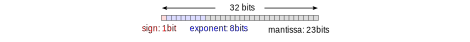
\includegraphics[width=1\linewidth]{figures/bits_single_precision.pdf}
\end{center}
$p=24$, $L=-126$, $U=127$
\begin{itemize}
\item Underfloat threshold = $2^{-126} \approx 10^{-38}$
\item Overflow threshold = $2^{128} \approx 10^{38}$
\end{itemize}

\item \textit{Double precision} (64 bits = 8 bytes) \lstinline{np.float64}
\begin{center}
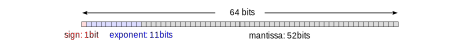
\includegraphics[width=1\linewidth]{figures/bits_double_precision.pdf}
\end{center}
$p=53$, $L=-1022$, $U=1023$
\begin{itemize}
\item Underfloat threshold = $2^{-1022} \approx 10^{-308}$
\item Overflow threshold = $2^{1024} \approx 10^{308}$
\end{itemize} 
\end{itemize}
\end{frame}

%%%%%%%%%%%%%%%%%%%%%%%%%%%%%%%%%%%%%%%%%%%%%%%%%%%%%%%%%%%%%%%%%%

\begin{frame}
\frametitle{Special values}
\textbf{Representation in IEEE 754 Standard}
\begin{itemize}
\item The number zero
$$
\texttt{s000 0000 0000 0000 0000 0000 0000 0000}
$$
$s$ = sign bit $\Rightarrow$ $+0$ ($s=1$) and $-0$ ($s=0$).
\item \texttt{NaN} (``not a number'') = result of invalid operations
$$
\texttt{s111 1111 1xxx xxxx xxxx xxxx xxxx xxxx}
$$ 
$x$ = any non-zero number, sign $s$ usually ignored
\item Infinity ($\pm\infty$)
$$
\texttt{s111 1111 1000 0000 0000 0000 0000 0000}
$$
\end{itemize}
\end{frame}

%%%%%%%%%%%%%%%%%%%%%%%%%%%%%%%%%%%%%%%%%%%%%%%%%%%%%%%%%%%%%%%%%%

\begin{frame}
\frametitle{Machine epsilon}
\textbf{Gaps between numbers in $\mathbb{F}$}
$$
x = \pm \left(d_0 + d_1\beta^{-1} + d_2\beta^{-1} + \dots+d_{p-1}\beta^{1-p}\right)\cdot\beta^E
$$
\begin{center}
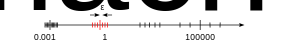
\includegraphics[width=\linewidth]{figures/floating_point_spacing.pdf}
\end{center}
$E$ $\Rightarrow$ $[2^E,2^{E+1}]$ discretised into $2^{p-1}$ pieces of size $2^{1-p}\cdot 2^E$\\[2ex]
\textbf{Machine epsilon} $E=0$ $\Rightarrow$ gap of numbers around $1$
$$
\varepsilon_{\text{mach}} := 2^{1-p} = \begin{cases}
2^{-23} \approx 10^{-7} & \text{in single precision}\\
2^{-52} \approx 2\cdot 10^{-16} & \text{in double precision}
\end{cases}
$$
\end{frame}

%%%%%%%%%%%%%%%%%%%%%%%%%%%%%%%%%%%%%%%%%%%%%%%%%%%%%%%%%%%%%%%%%%

\begin{frame}
\frametitle{Machine epsilon}
\textbf{Alternative definitions}
\begin{itemize}
\item \textit{``Gap of numbers around $1$''}
$$
\varepsilon_{\text{mach}} = 2^{1-p}
$$
\item \textit{``Smallest positive number $x\in \mathbb{F}$ that can be added to $1$ such that (after rounding to $\mathbb{F}$) the result differs from $1$''}
$$
\varepsilon_{\text{mach}} := \min_{x\in\mathbb{F},x>0}\{x: \mathcal{R}_{\mathbb{F}}(1+x)\neq 1\}
$$
\item \textit{``Relative size of rounding errors or the relative accuracy of floating point operations.''}
$$
\frac{|\mathcal{R}_{\mathbb{F}}(z)-z|}{|z|} \sim \varepsilon_{\text{mach}}.
$$
\end{itemize}
{\footnotesize NB: sometimes $\varepsilon_{\text{mach}}$ is defined with an additional factor $2$ in the literature.}
\end{frame}

%%%%%%%%%%%%%%%%%%%%%%%%%%%%%%%%%%%%%%%%%%%%%%%%%%%%%%%%%%%%%%%%%%

\begin{frame}
\frametitle{Rounding errors}
\textbf{Example 1} (harmless)
\begin{xalignat*}{2}
x&=4.7\cdot 10^{-16}\in\mathbb{F},& y&=2.9\cdot 10^{-16}\in\mathbb{F}
\end{xalignat*}
$$
z=x-y=1.8\cdot 10^{-16} = \mathcal{R}_{\mathbb{F}}(z) \in\mathbb{F}
$$
$$
\frac{\mathcal{R}_{\mathbb{F}}(z)-z}{z} = \frac{x-y-z}{z} = \frac{(4.7 -2.9 - 1.8)\cdot10^{-16}}{1.8\cdot 10^{-16}} = 0.
$$
$\Rightarrow$ small (zero) relative error if $x\sim y \sim x-y$
\end{frame}

%%%%%%%%%%%%%%%%%%%%%%%%%%%%%%%%%%%%%%%%%%%%%%%%%%%%%%%%%%%%%%%%%%

\begin{frame}
\frametitle{Rounding errors}
\textbf{Example 2} (subtracting two numbers that are very close)
\begin{xalignat*}{2}
x&=4.7\cdot 10^{-16}\in\mathbb{F},& y&=2.9\cdot 10^{-16}\in\mathbb{F}
\end{xalignat*}
\begin{xalignat*}{3}
x'&=1+x,& y'&=1+y,& z'&=x'-y'
\end{xalignat*}
In exact arithmetic: $z'=x'-y'=x-y$, but
$$
\begin{aligned}
\mathcal{R}_{\mathbb{F}}(x')&=1.00000000000000044\\
\mathcal{R}_{\mathbb{F}}(y')&=1.00000000000000022
\end{aligned}
$$
The \textbf{relative error} of $z'$
$$
\begin{aligned}
\frac{\mathcal{R}_{\mathbb{F}}(z')-z}{z} &= \frac{\mathcal{R}_{\mathbb{F}}(x')-\mathcal{R}_{\mathbb{F}}(y')-z}{z}\\
&= \frac{(4.4 - 2.2 - 1.8)\cdot10^{-16}}{1.8\cdot 10^{-16}} = \frac{0.4}{1.8} \approx 23\%
\end{aligned}
$$
Observe: $z'\ll x'\sim y'$ in contrast to $z\ll x\sim y$ (Example 1)
\end{frame}

%%%%%%%%%%%%%%%%%%%%%%%%%%%%%%%%%%%%%%%%%%%%%%%%%%%%%%%%%%%%%%%%%%

\begin{frame}
\frametitle{Rounding errors}
\textbf{Example 3} (adding two numbers of very different size)\\[1ex]
Linear system
$$
\begin{pmatrix}
0 & 1 \\ 1 & 1 
\end{pmatrix}
\begin{pmatrix}
x_0 \\ x_1
\end{pmatrix}
=
\begin{pmatrix}
1 \\ 0
\end{pmatrix}
\qquad\text{$\Rightarrow$ solution: $x_0=-1$, $x_1=1$}
$$
perturbed problem
$$
\begin{pmatrix}
-10^{-20} & 1 \\ 1 & 1 
\end{pmatrix}
\begin{pmatrix}
x_0 \\ x_1
\end{pmatrix}
=
\begin{pmatrix}
1 \\ 0
\end{pmatrix}
$$
Solution
\begin{xalignat*}{2}
  x_0&=-\frac{1}{1+10^{-20}}\approx -1,&
  x_1&=\frac{1}{1+10^{-20}}\approx 1
\end{xalignat*}
\end{frame}

%%%%%%%%%%%%%%%%%%%%%%%%%%%%%%%%%%%%%%%%%%%%%%%%%%%%%%%%%%%%%%%%%%

\begin{frame}
\frametitle{Rounding errors}
\textbf{Solution of perturbed problem}
$$
\begin{aligned}
-10^{-20} x_0 + x_1 &= 1\quad (\dagger)\\
x_0 + x_1 &= 0\quad (\star)
\end{aligned}
$$
$10^{20}\cdot (\dagger ) + (\star)$
$$
\begin{aligned}
-10^{-20} x_0 + x_1 &= 1\\
\underbrace{(1+10^{20})}_{\approx 10^{20}} x_1 &= 10^{20}
\end{aligned}
$$
$\Rightarrow$ in double precision arithmetic
$$
\begin{aligned}
-10^{-20} x_0 + x_1 &= 1\\
10^{20} x_1 &= 10^{20},
\end{aligned}
$$
$$
\Rightarrow \quad x_1 = 1 \quad \Rightarrow\quad  x_1 = 1 -10^{-20} x_0 + 1 = 1 \quad \Rightarrow \quad x_0 = 0
$$
Not close to solution $x_0=-1$, $x_1=1$ of unperturbed system!
\end{frame}

%%%%%%%%%%%%%%%%%%%%%%%%%%%%%%%%%%%%%%%%%%%%%%%%%%%%%%%%%%%%%%%%%%

\begin{frame}
\frametitle{Rounding errors}
\textbf{Fix}
$$
\begin{aligned}
-10^{-20} x_0 + x_1 &= 1\quad (\dagger)\\
x_0 + x_1 &= 0\quad (\star)
\end{aligned}
$$
$(\star ) - (\dagger)$
$$
\begin{aligned}
\underbrace{(1+10^{-20})}_{\approx 1} x_0 &= -1\\
x_0 + x_1 &= 0
\end{aligned}
$$
\begin{xalignat*}{2}
\Rightarrow \quad x_0 &= -1, & x_1 &= 1
\end{xalignat*}
This is what \lstinline{numpy.linalg.solve()} will do
\end{frame}

%%%%%%%%%%%%%%%%%%%%%%%%%%%%%%%%%%%%%%%%%%%%%%%%%%%%%%%%%%%%%%%%%%

\begin{frame}
\frametitle{Rounding errors}
\textbf{Example 4} (ill-conditioned matrix)\\[1ex]
Solve $A\boldsymbol{u}=\boldsymbol{b}$
$$
\begin{aligned}
A &= \begin{pmatrix}
1+\frac{1}{\sqrt{2}} + \frac{2+\sqrt{2}}{4}\epsilon & \frac{1}{\sqrt{2}}-\frac{\sqrt{2}}{4}\epsilon\\[1ex]
\frac{1}{\sqrt{2}}-\frac{\sqrt{2}}{4}\epsilon & 1-\frac{1}{\sqrt{2}}+\frac{2-\sqrt{2}}{4}\epsilon
\end{pmatrix}\qquad\text{$\epsilon>0$}
\\
&\approx
{\tiny%
\begin{pmatrix}
1.7071067811865475 + 0.8535533905932737 \cdot\epsilon & 0.7071067811865475 - 0.3535533905932738 \cdot\epsilon \\
0.7071067811865475 - 0.3535533905932738 \cdot\epsilon & 0.2928932188134525 + 0.1464466094067262\cdot\epsilon
\end{pmatrix}}
\end{aligned}
$$
$$
\boldsymbol{b} = \begin{pmatrix}
\frac{\sqrt{2+\sqrt{2}}+\sqrt{2-\sqrt{2}}}{2}\\[1ex]
\frac{\sqrt{2+\sqrt{2}}-\sqrt{2-\sqrt{2}}}{2}
\end{pmatrix}
\approx
{\footnotesize%
\begin{pmatrix}
1.3065629648763766\\0.5411961001461970
\end{pmatrix}}
$$
xact solution, independent of $\epsilon$
$$
\boldsymbol{u}_{\text{exact}} = 
\begin{pmatrix}
\frac{\sqrt{2 - \sqrt{2}}}{2}\\[1ex]
\frac{\sqrt{2 + \sqrt{2}}}{2}
\end{pmatrix}
\approx 
{\footnotesize%
\begin{pmatrix}
0.3826834323650897\\0.9238795325112867
\end{pmatrix}}
$$
\end{frame}

%%%%%%%%%%%%%%%%%%%%%%%%%%%%%%%%%%%%%%%%%%%%%%%%%%%%%%%%%%%%%%%%%%

\begin{frame}[fragile]
\frametitle{Rounding errors}

\begin{minipage}{0.45\linewidth}
\begin{lstlisting}
u = np.linalg.solve(A,b)
\end{lstlisting}
\end{minipage}
\hfill
\begin{minipage}{0.45\linewidth}
$\boldsymbol{u}_{\text{exact}} 
\approx 
{\footnotesize%
\begin{pmatrix}
0.3826834323650897\\0.9238795325112867
\end{pmatrix}}$
\end{minipage}\\
 \begin{center}
  \renewcommand{\arraystretch}{1.5}
\begin{tabular}{cccc}  
  \hline
$\epsilon$ & solution $\boldsymbol{u}$ & $\frac{\|\boldsymbol{u}-\boldsymbol{u}_{\text{exact}}\|_2}{\|\boldsymbol{u}_{\text{exact}}\|_2}$ & $\text{cond}(A)$\\
\hline\hline
  $10^{-3}$ & ${\tiny\begin{pmatrix}0.3826834323650560 \\ 0.9238795325113685\end{pmatrix}}$ &  $8.8408\cdot 10^{-14}$  & $4\cdot 10^3$ \\
  $10^{-6}$ & ${\tiny\begin{pmatrix}0.3826834323171860 \\0.9238795326269368\end{pmatrix}}$ & $1.2518\cdot 10^{-10}$ & $4\cdot 10^6$ \\
  $10^{-9}$ & ${\tiny\begin{pmatrix}0.3826834290672392 \\0.9238795404730024\end{pmatrix}}$ & $8.6177\cdot 10^{-9}$ & $4\cdot 10^9$ \\
  $10^{-12}$ & ${\tiny\begin{pmatrix}0.3826776593455781 \\ 0.9238934698132879\end{pmatrix}}$ & $1.5086\cdot10^{-5}$ & $4\cdot 10^{12}$ \\
  $10^{-15}$ & ${\tiny\begin{pmatrix}0.3888090807546386 \\0.9090909090909092\end{pmatrix}}$ & $1.6007\cdot10^{-2}$ & $4\cdot 10^{15}$ \\
  $8\cdot 10^{-16}$ & ${\tiny\begin{pmatrix} 0.2919799363037854 \\1.1428571428571428\end{pmatrix}}$ & $2.3702\cdot 10^{-1}$ & $5\cdot 10^{15}$ \\
  $4\cdot 10^{-16}$ & ${\tiny\begin{pmatrix} -0.0630602600160104 \\ 2.0000000000000000\end{pmatrix}}$ & $1.1648$ & $10^{16}$ \\
  \hline
\end{tabular}
\end{center}
condition number $\text{cond}(A) = \lambda_+/\lambda_-\approx 4/\epsilon$
\end{frame}

%%%%%%%%%%%%%%%%%%%%%%%%%%%%%%%%%%%%%%%%%%%%%%%%%%%%%%%%%%%%%%%%%%

\begin{frame}
\frametitle{Backward error analysis}
Solution $\boldsymbol{u}\in\mathbb{R}^n$ in exact arithmetic satisfies
$$
A\boldsymbol{u} = \boldsymbol{b}
$$
Rounding errors $\Rightarrow$ computed solution $\boldsymbol{u}'=\boldsymbol{u}+\delta\boldsymbol{u}$ solves
$$
(A+\delta A)(\boldsymbol{u}+\delta\boldsymbol{u}) = \boldsymbol{b} + \delta\boldsymbol{b}
\qquad\text{\footnotesize(assume $\delta\boldsymbol{b}=0$ for simplicity)}
$$
Goal: derive \textbf{bound} on $\delta\boldsymbol{u}$ \\[1ex]
\end{frame}

%%%%%%%%%%%%%%%%%%%%%%%%%%%%%%%%%%%%%%%%%%%%%%%%%%%%%%%%%%%%%%%%%%

\begin{frame}
\frametitle{Backward error analysis}
\textbf{Norms}
$$
\begin{aligned}
\|\boldsymbol{w}\|_\infty &:= \max_{i=0,\dots,n-1} |w_i|,\\
\|A\|_\infty &:= \max_{\boldsymbol{w}\in\mathbb{R}^n,\boldsymbol{w}\neq \boldsymbol{0}} \frac{\|A\boldsymbol{w}\|_\infty}{\|\boldsymbol{w}\|_\infty} = \max_{0\le i < n} \sum_{j=0}^{n-1} |A_{ij}|
\end{aligned}
$$
$\Rightarrow$ $\|A\boldsymbol{w}\|_\infty\le \|A\|_\infty\|\boldsymbol{w}\|_\infty$ and $\|AB\|_\infty\le\|A\|_\infty\|B\|_\infty$.
\end{frame}

%%%%%%%%%%%%%%%%%%%%%%%%%%%%%%%%%%%%%%%%%%%%%%%%%%%%%%%%%%%%%%%%%%

\begin{frame}
\frametitle{Backward error analysis}
Condition number of matrix $A$
$$
\text{cond}(A) := \|A^{-1}\|_\infty\|A\|_\infty.
$$
($=\lambda_{\text{max}}/\lambda_{\text{min}}$ for real-valued SPD matrix)\\[2ex]
\textbf{Theorem 1}\\
If the $n\times n$ matrix $A$ is non-singular and if $\delta A$ is sufficiently small
$$
\|\delta A\|_{\infty} \|A^{-1}\|_\infty \le \frac{1}{2}
$$
then $A+\delta A$ is non-singular and
$$
\frac{\|\delta\boldsymbol{u}\|_\infty}{\|\boldsymbol{u}\|_\infty} \le 2\;\text{cond}(A) \frac{\|\delta A\|_\infty}{\|A\|_\infty}
$$
Proof (not examinable): see lecture notes
\end{frame}

%%%%%%%%%%%%%%%%%%%%%%%%%%%%%%%%%%%%%%%%%%%%%%%%%%%%%%%%%%%%%%%%%%

\begin{frame}
\frametitle{Backward error analysis}
Gaussian elimination
$$
\frac{\|\delta A\|_\infty}{\|A\|_\infty} \le n\cdot \varepsilon_{\text{mach}}\cdot G(A),
$$
$G(A)$ = "well-behaved" number\\[2ex]

\textbf{Theorem 2}\\
Under the conditions of Theorem 1 and if Gaussian elimination is used to solve the linear system, the error $\delta \boldsymbol{u}$ can be bounded

$$
\frac{\|\delta\boldsymbol{u}\|_\infty}{\|\boldsymbol{u}\|_\infty} \le 2\cdot G(A)\cdot n\cdot \text{cond}(A)\cdot \varepsilon_{\text{mach}}
$$
proportional to
\begin{itemize}
\item  machine epsilon $\varepsilon_{\text{mach}}$
\item problem size $n$
\item condition number $\text{cond}(A)$
\end{itemize}
\end{frame}

%%%%%%%%%%%%%%%%%%%%%%%%%%%%%%%%%%%%%%%%%%%%%%%%%%%%%%%%%%%%%%%%%%

\begin{frame}
\frametitle{Estimating the error}
Generally impossible to compute the error $\delta\boldsymbol{u}=\boldsymbol{u}'-\boldsymbol{u}$\\[1ex]
\textbf{Residual}
$$
\boldsymbol{r}:=\boldsymbol{b}-A\boldsymbol{u}'=A\delta\boldsymbol{u} \qquad\text{($= 0$ if $\delta\boldsymbol{u}=0$)}
$$
Unfortunately
$$
\|\boldsymbol{r}\|_\infty\ll 1 \quad\nRightarrow\quad \|\delta\boldsymbol{u}\|_\infty\ll 1
$$
Properties of $\|\cdot\|_\infty$
\begin{xalignat*}{2}
\|\boldsymbol{b}\|_\infty &\le \|A\|_\infty \|\boldsymbol{u}\|_\infty, & \|\delta\boldsymbol{u}\|_\infty &\le \|A^{-1}\|_\infty \|\boldsymbol{r}\|_\infty
\end{xalignat*}
$$
\Rightarrow\quad\frac{\|\delta \boldsymbol{u}\|_\infty}{\|\boldsymbol{u}\|_\infty} 
\le \|A^{-1}\|_\infty\| \boldsymbol{r}\|_\infty \frac{\|A\|_\infty}{\|\boldsymbol{b}\|_\infty} = \text{cond}(A)\frac{\|\boldsymbol{r}\|_\infty}{\|\boldsymbol{b}\|_\infty}
$$
In the absence of any other information $\|\boldsymbol{r}\|_\infty$ is a useful quantity to measure.
\end{frame}

%%%%%%%%%%%%%%%%%%%%%%%%%%%%%%%%%%%%%%%%%%%%%%%%%%%%%%%%%%%%%%%%%%

\begin{frame}
\frametitle{Error for finite element problem}
Recall: $A^{(h)}\vec{u}^{(h)}=\vec{b}^{(h)}$ on $\widehat{K}$\\[2ex]
\begin{minipage}{0.475\linewidth}
\begin{center}
\includegraphics[width=\linewidth]{figures/error_reference_triangle.png}\\\textcolor{white}{X}
\end{center}
\end{minipage}
\hfill
\begin{minipage}{0.475\linewidth}
\begin{center}
\includegraphics[width=\linewidth]{figures/conditioning_reference_triangle.png}\\
$n_{\text{dof}}\cdot \text{cond}(A^{(h)})$
\end{center}
\end{minipage}\\
Typical problem in Scientific Computing
\begin{itemize}
\item Large $n_{\text{dof}} \gg 1$
\item Ill-conditioned $\text{cond}(A^{(h)})$
\end{itemize}
\end{frame}

%%%%%%%%%%%%%%%%%%%%%%%%%%%%%%%%%%%%%%%%%%%%%%%%%%%%%%%%%%%%%%%%%%

\section{Unstructured meshes}

%%%%%%%%%%%%%%%%%%%%%%%%%%%%%%%%%%%%%%%%%%%%%%%%%%%%%%%%%%%%%%%%%%

\begin{frame}
  \tableofcontents[currentsection]
\end{frame}

%%%%%%%%%%%%%%%%%%%%%%%%%%%%%%%%%%%%%%%%%%%%%%%%%%%%%%%%%%%%%%%%%%

\begin{frame}
  \frametitle{Unstructured meshes}
  $d$-dimensional manifold $\Omega\subset \mathbb{R}^D$ (this unit: $D=d=2$)\\
  \textbf{Mesh}
  $$
  \Omega \approx \Omega_h = \left\{\text{topological entities}\right\}
  $$
\begin{minipage}{0.6\linewidth}
 \begin{center}
  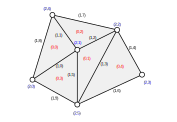
\includegraphics[width=\linewidth]{figures/simple_mesh.pdf}
 \end{center}
\end{minipage}
\hfill
\begin{minipage}{0.25\linewidth} 
  label = (c,id)  
 \end{minipage}
\begin{center}
  \begin{tabular}{ccc}
   \hline 
 topological entity & dim $d'$ & co-dim $c=d-d'$\\
\hline\hline
 cell (triangle) $K$ & $2$ & $0$\\
 facet (edge) $F$    & $1$ & $1$\\
 vertex (point) $v$  & $0$ & $2$\\
  \end{tabular}
\end{center}
\end{frame}

%%%%%%%%%%%%%%%%%%%%%%%%%%%%%%%%%%%%%%%%%%%%%%%%%%%%%%%%%%%%%%%%%%

\begin{frame}
  \frametitle{Topology}
  \textbf{Topology}
  \begin{center}
  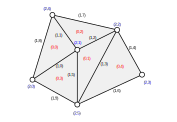
\includegraphics[width=0.6\linewidth]{figures/simple_mesh.pdf}
 \end{center}
  \begin{itemize}
\item Cell $(0,1)$ has facets $(1,3), (1,2), (1,5)$
\item Facet $(1,2)$ has the endpoints $(2,1), (2,2)$
  \end{itemize}
\end{frame}

%%%%%%%%%%%%%%%%%%%%%%%%%%%%%%%%%%%%%%%%%%%%%%%%%%%%%%%%%%%%%%%%%%

\begin{frame}
  \frametitle{Connectivity matrices}
  \textbf{Topology}\\
  Encode topology in two matrices  
 \begin{itemize}
\item $n_{\text{cell}}\times 3$ matrix $I^{K\rightarrow F}$
$$
I^{K\rightarrow F}_{\alpha\beta} = \text{index of $\beta$-th facet of cell $\alpha$}
$$
\item $n_{\text{facet}}\times 2$ matrix $I^{F\rightarrow v}$
$$
I^{F\rightarrow v}_{\beta\gamma} = \text{index of $\gamma$-th vertex of facet $\beta$}.
$$
 \end{itemize}  
  \begin{minipage}{0.475\linewidth}    
\textbf{Ordering conventions}
\begin{itemize}
\item $I^{K\rightarrow F}_{\alpha0}$, $I^{K\rightarrow F}_{\alpha1}$ and $I^{K\rightarrow F}_{\alpha2}$ arranged counter-clockwise
\item $I^{F\rightarrow v}_{\beta0} < I^{F\rightarrow v}_{\beta1}$
\end{itemize}
\end{minipage}
  \hfill
  \begin{minipage}{0.475\linewidth}
    \begin{center}
  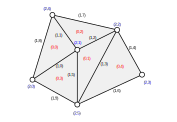
\includegraphics[width=\linewidth]{figures/simple_mesh.pdf}
 \end{center}
  \end{minipage}
\end{frame}

%%%%%%%%%%%%%%%%%%%%%%%%%%%%%%%%%%%%%%%%%%%%%%%%%%%%%%%%%%%%%%%%%%

\begin{frame}
  \frametitle{Connectivity matrices}
  Derived $n_{\text{cell}}\times 3$ matrix $I^{K\rightarrow v}$ 
$$
I^{K\rightarrow v}_{\alpha\gamma} = \text{index of $\gamma$-th vertex of cell $\alpha$}.
$$

Number vertices counter-clockwise such that the $\gamma$-th vertex lies opposite the $\gamma$-the facet
$$
\begin{aligned}
I^{K\rightarrow v}_{\alpha\gamma} \not\in \{I^{F\rightarrow v}_{\beta0},I^{F\rightarrow v}_{\beta1}\}\quad\text{for $\beta =I^{K\rightarrow F}_{\alpha\gamma}$}
\end{aligned}.
$$
Consistent with the numbering of unknowns on $\widehat{K}$
  \begin{center}
  \includegraphics[width=0.4\linewidth]{figures/reference_triangle_small.pdf}
  \end{center}

\end{frame}

%%%%%%%%%%%%%%%%%%%%%%%%%%%%%%%%%%%%%%%%%%%%%%%%%%%%%%%%%%%%%%%%%%

\begin{frame}
  \frametitle{Example mesh I}
  \begin{center}
  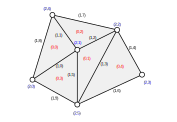
\includegraphics[width=0.7\linewidth]{figures/simple_mesh.pdf}
 \end{center}
$$
\begin{aligned}
I^{K\rightarrow F} &= \begin{pmatrix}
0 & 3 & 1 & 0 & 3 \\
1 & 2 & 2 & 9 & 6 \\
8 & 5 & 7 & 5 & 4
\end{pmatrix}^{\top}\qquad I^{K\rightarrow v} = \begin{pmatrix}
4 & 1 & 2 & 5 & 3 \\
0 & 5 & 4 & 1 & 2 \\
1 & 2 & 1 & 0 & 5
\end{pmatrix}^{\top}
\\
I^{F\rightarrow v} &= \begin{pmatrix}
0 & 1 & 1 & 2 & 2 & 1 & 3 & 2 & 0 & 0 \\
1 & 4 & 2 & 5 & 3 & 5 & 5 & 4 & 4 & 5
\end{pmatrix}^{\top}
\end{aligned}
$$
\end{frame}

%%%%%%%%%%%%%%%%%%%%%%%%%%%%%%%%%%%%%%%%%%%%%%%%%%%%%%%%%%%%%%%%%%

\begin{frame}[fragile]
  \frametitle{Example mesh II}
\begin{center}
  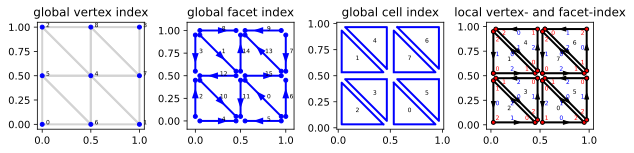
\includegraphics[width=1\linewidth]{figures/rectangle_mesh_wide.pdf}\\
  Generated with \lstinline{rectangle_mesh(Lx=1.0, Ly=1.0, nref=1)}
 \end{center}
$$
\setcounter{MaxMatrixCols}{20}
\begin{aligned}
I^{K\rightarrow F} &= \begin{pmatrix}
5 & 1 & 2 & 10 & 8 & 0 & 7 & 13\\
0 & 3 & 4 & 11 & 1 & 6 & 9 & 14\\
11 & 12 & 10 & 12 & 14 & 15 & 13 & 15
\end{pmatrix}^{\top}
\\
I^{F\rightarrow v} &= \begin{pmatrix}
1 & 2 & 0 & 2 & 0 & 1 & 1 & 3 & 2 & 3 & 5 & 4 & 4 & 7 & 4 & 4\\
4 & 4 & 5 & 5 & 6 & 6 & 7 & 7 & 8 & 8 & 6 & 6 & 5 & 8 & 8 & 7
\end{pmatrix}^{\top}
\\
I^{K\rightarrow v} &= \begin{pmatrix}
4 & 5 & 6 & 4 & 4 & 7 & 8 & 4\\
6 & 4 & 5 & 5 & 8 & 4 & 7 & 7\\
1 & 2 & 0 & 6 & 2 & 1 & 3 & 8
\end{pmatrix}^{\top}
\end{aligned}
$$

\end{frame}

%%%%%%%%%%%%%%%%%%%%%%%%%%%%%%%%%%%%%%%%%%%%%%%%%%%%%%%%%%%%%%%%%%

\begin{frame}[fragile]
  \frametitle{Implementation}
Class \lstinline{Mesh} encodes mesh topology
\begin{itemize}
\item number of cells ($=n_{\text{cell}}$), facets ($=n_{\text{facet}}$), vertices ($=n_{\text{vertex}}$):\\
properties \lstinline{ncells}, \lstinline{nfacets}, \lstinline{nvertices} 
\item $I^{K\rightarrow F}$: \lstinline{cell2facet}, $I^{K\rightarrow F}_{\alpha\beta} =$ \lstinline{cell2facet[alpha][beta]} 
\item $I^{F\rightarrow v}$: \lstinline{facet2vertex}, $I^{F\rightarrow v}_{\beta\gamma} =$ \lstinline{facet2vertex[beta][gamma]}
\item $I^{K\rightarrow v}$: \lstinline{cell2vertex}, $I^{K\rightarrow v}_{\alpha\gamma} =$ \lstinline{cell2vertex[alpha][gamma]}\\
{}\quad{\footnotesize (implemented as a \lstinline{@functools.cached_property})}
\item Coordinates of mesh vertices: $n_{\text{vertex}}\times 2$ array \lstinline{vertices}
\end{itemize}
\vspace{2ex}
Initialise with
\begin{lstlisting}
mesh = Mesh(vertices, cell2facet, facet2vertex)
\end{lstlisting}
\begin{minipage}{0.35\linewidth}
then refine cells with
\begin{lstlisting}
mesh.refine(nref)
\end{lstlisting}
\end{minipage}
\hfill
\begin{minipage}{0.6\linewidth}
\begin{center}
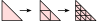
\includegraphics[width=0.9\linewidth]{figures/mesh_refinement.pdf}
\end{center}
\end{minipage}
\end{frame}

%%%%%%%%%%%%%%%%%%%%%%%%%%%%%%%%%%%%%%%%%%%%%%%%%%%%%%%%%%%%%%%%%%

\begin{frame}[fragile]
  \frametitle{Implementation}
\textbf{Factory methods}
\begin{itemize}
\item \textit{Rectangle mesh}: triangulation of $[0,L_x]\times[0,L_y]$\\
\lstinline{rectangle_mesh(Lx=1.0, Ly=1.0, nref=0)}\\
$n_{\text{ref}}$ refinements $\Rightarrow$ $n_{\text{cells}} = 2^{n_{\text{ref}}+1}$
\item \textit{Triangle mesh}: triangulation of triangle defined by \lstinline{corners}\\
\lstinline{triangle_mesh(corners=None, nref=0)}\\
$n_{\text{ref}}$ refinements $\Rightarrow$ $n_{\text{cells}} = 2^{n_{\text{ref}}}$
\end{itemize}
\vspace{2ex}
\textbf{Examples} ($n_{\text{ref}}=2$)\\[1ex]
\begin{minipage}{0.45\linewidth}
  \begin{center}
    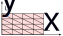
\includegraphics[width=0.8\linewidth]{figures/rectangle_mesh_schematic.pdf}
  \end{center}
\end{minipage}
\hfill
\begin{minipage}{0.45\linewidth}
  \begin{center}
    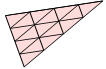
\includegraphics[width=0.7\linewidth]{figures/triangle_mesh_schematic.pdf}
  \end{center}
\end{minipage}
\end{frame}

%%%%%%%%%%%%%%%%%%%%%%%%%%%%%%%%%%%%%%%%%%%%%%%%%%%%%%%%%%%%%%%%%%

\section{Function spaces}

%%%%%%%%%%%%%%%%%%%%%%%%%%%%%%%%%%%%%%%%%%%%%%%%%%%%%%%%%%%%%%%%%%

\begin{frame}
  \tableofcontents[currentsection]
\end{frame}

%%%%%%%%%%%%%%%%%%%%%%%%%%%%%%%%%%%%%%%%%%%%%%%%%%%%%%%%%%%%%%%%%%

\begin{frame}
  \frametitle{Pullback to $\widehat{K}$}
  \textbf{Images of reference cell}\\[1ex]
Cell $K$ = image of $\widehat{K}$ under bijective map
$$
X_K:\widehat{K}\rightarrow K\subset \Omega\subset \mathbb{R}^2
$$
\begin{center}
  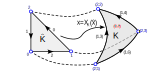
\includegraphics[width=0.8\linewidth]{figures/reference_mapping.pdf}
\end{center}
\textbf{Pullback} $\widehat{f}:\widehat{K}\rightarrow \mathbb{R}$ of $f:K\rightarrow \mathbb{R}$ under $X_K$
$$
\widehat{f} = f\circ X_K\quad\Leftrightarrow\quad
\widehat{f}(\widehat{x}) = f(X_K(\widehat{x}))\qquad\text{for all $\widehat{x}\in\widehat{K}$}.
$$
\end{frame}

%%%%%%%%%%%%%%%%%%%%%%%%%%%%%%%%%%%%%%%%%%%%%%%%%%%%%%%%%%%%%%%%%%

\begin{frame}
  \frametitle{Arrangement of unknowns}
  \textbf{Function space $\mathcal{V}_h\subset H^1(\Omega_h)$ on mesh $\Omega_h$}\\
  Pullback of the function $u|_K$ is a polynomial:
$$
\mathcal{V}_h := \{u\in H^1(\Omega_h): u|_K(x) = \widehat{u}_K(\widehat{x}),\;\;x=X_K(\widehat{x}),\;\;\widehat{u}_K\in\mathcal{P}_p(\widehat{K})\}
$$
Can use basis $\mathcal{P}_p(\widehat{K})$ to represent the functions $\widehat{u}_K$\\
\textbf{Continuity across facets}\\
$$
u_h(x) = \sum_{\ell_{\text{global}}=0}^{n-1} u^{(h)}_{\ell_{\text{global}}} \Phi^{(h)}_{\ell_{\text{global}}}(x)
$$
\begin{itemize}
\item Global basis functions $\Phi^{(h)}_{\ell_{\text{global}}}$
\item Global dof-vector $u^{(h)}_{\ell_{\text{global}}}$
\end{itemize}
Need to associate the indices $\ell_{\text{global}}$ with the correct mesh entities.
\end{frame}

%%%%%%%%%%%%%%%%%%%%%%%%%%%%%%%%%%%%%%%%%%%%%%%%%%%%%%%%%%%%%%%%%%

\begin{frame}
  \frametitle{Gluing together basis functions}
  \textbf{Global basis functions = $\boldsymbol{\sum}$ local basis function}
  \begin{center}
  
\includegraphics[width=0.6\linewidth]{figures/continuity_vertex.pdf}\\
  {\footnotesize $\Phi^{(h)}_{\ell_{\text{global}}}$ associated with vertex}
  \end{center}
  \begin{center}
  
\includegraphics[width=0.6\linewidth]{figures/continuity_facet.pdf}\\
  {\footnotesize $\Phi^{(h)}_{\ell_{\text{global}}}$ associated with facet}
  \end{center}
\end{frame}

%%%%%%%%%%%%%%%%%%%%%%%%%%%%%%%%%%%%%%%%%%%%%%%%%%%%%%%%%%%%%%%%%%

\begin{frame}
  \frametitle{Arrangement of unknowns}
  \textbf{Mesh} with $n_{\text{vertex}}$ vertices, $n_{\text{facet}}$ facets and $n_{\text{cell}}$ cells\\[1ex]
  \textbf{Finite element}
  \begin{center}
    \renewcommand{\arraystretch}{1.2}
  \begin{tabular}{ccc}
    \hline
    entity & local unknowns & total unknowns \\
    \hline\hline
    vertex & $\nu_{\text{vertex}}$ & $N_{\text{vertex}} = n_{\text{vertex}}\cdot \nu_{\text{vertex}}$ \\ 
    facet & $\nu_{\text{facet}}$ & $N_{\text{facet}} = n_{\text{facet}}\cdot \nu_{\text{facet}}$ \\
    cell (interior) & $\nu_{\text{interior}}$  & $N_{\text{interior}} = n_{\text{cell}}\cdot \nu_{\text{interior}}$\\
    \hline 
    & total & $N_{\text{vertex}}+N_{\text{facet}}+N_{\text{interior}}$\\
    \hline
  \end{tabular}
  \end{center}
  
\end{frame}

%%%%%%%%%%%%%%%%%%%%%%%%%%%%%%%%%%%%%%%%%%%%%%%%%%%%%%%%%%%%%%%%%%

\begin{frame}
  \frametitle{Arrangement of unknowns}
  \textbf{Ordering of unknowns}
  {\footnotesize
  \begin{itemize}
    \item vertex $\gamma$:\\
      $\ell_{\text{global}}\in\{\gamma\cdot \nu_{\text{vertex}},\dots,(\gamma+1)\cdot \nu_{\text{vertex}}-1\}$
    \item facet $\beta$ (following orientation):\\
      $\ell_{\text{global}}\in\{N_{\text{vertex}}+\beta\cdot \nu_{\text{facet}},\dots,N_{\text{vertex}}+(\beta+1)\cdot \nu_{\text{facet}}-1\}$
    \item cell $\alpha$:\\
      $\ell_{\text{global}}\in\{N_{\text{vertex}}+N_{\text{facet}}+\alpha\cdot \nu_{\text{interior}},\dots,N_{\text{vertex}}+N_{\text{facet}}+(\alpha+1)\cdot \nu_{\text{interior}}-1\}$ 
  \end{itemize}
  }
\begin{center}
  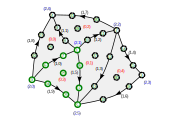
\includegraphics[width=0.6\linewidth]{figures/simple_mesh_with_dof_numbers.pdf}
  \end{center}
\end{frame}

%%%%%%%%%%%%%%%%%%%%%%%%%%%%%%%%%%%%%%%%%%%%%%%%%%%%%%%%%%%%%%%%%%

\begin{frame}
  \frametitle{Local-to-global map}
  \begin{center}
    \begin{minipage}{0.4\linewidth}
      \textbf{Local-to-global map}
  $$(\alpha,\ell) \mapsto \ell_{\text{global}}$$
    \end{minipage}\hfill
    \begin{minipage}{0.55\linewidth}
      \begin{center}
        
\includegraphics[width=0.9\linewidth]{figures/continuity_facet_oriented.pdf}
      \end{center}
    \end{minipage}
  \end{center}
\begin{enumerate}
\item For given $\ell$ invert FE dof-map $\ell = \mu_{\text{dof}}(E,\rho,j)$:
\begin{itemize}
  \item entity type $E$ (cell, facet or vertex) 
  \item index $\rho$ of entity on $\widehat{K}$ 
  \item index $j$ of dof on $E_\rho$.
\end{itemize}
\item Map $(E,\rho,j), \alpha \mapsto \ell_{\text{global}}$
\begin{itemize}
   \item If $E=\text{vertex}$: $\ell_{\text{global}} = \gamma\cdot \nu_{\text{vertex}}+j$ where $\gamma=I^{K\rightarrow v}_{\alpha\rho}$
   \item If $E=\text{facet}$: $\ell_{\text{global}} = N_{\text{vertex}}+\beta\cdot \nu_{\text{facet}}+\widetilde{j}$ where $\beta=I^{K\rightarrow F}_{\alpha\rho}$\\
   $\widetilde{j}\in\{j,\nu_{\text{facet}}-1-j\}$ depending on orientation 
  \item If $E=\text{cell}$: $\ell_{\text{global}} = N_{\text{vertex}}+N_{\text{facet}}+\alpha\cdot \nu_{\text{interior}}+j$
\end{itemize}
\end{enumerate}
\end{frame}

%%%%%%%%%%%%%%%%%%%%%%%%%%%%%%%%%%%%%%%%%%%%%%%%%%%%%%%%%%%%%%%%%%

\begin{frame}[fragile]
  \frametitle{Implementation in Python}
  \textbf{Function spaces}\\
  Class \lstinline{FunctionSpace(mesh,finiteelement)}
  \begin{itemize}
  \item property \lstinline{ndof}: total number of unknowns $N_{\text{vertex}}+N_{\text{facet}}+N_{\text{interior}}$
  \item method \lstinline{local2global(self, alpha, ell)}: map $(\alpha,\ell)\mapsto\ell_{\text{global}}$ {\footnotesize($\ell$ = integer or list of integers)}
  \end{itemize}
\end{frame}

%%%%%%%%%%%%%%%%%%%%%%%%%%%%%%%%%%%%%%%%%%%%%%%%%%%%%%%%%%%%%%%%%%

\begin{frame}[fragile]
  \frametitle{Implementation in Python}
  \textbf{Functions} $u_h\in\mathcal{V}_h$\\[1ex]
  Class \lstinline{Function(functionspace)}
  \begin{itemize}
    \item property \lstinline{functionspace}
    \item property \lstinline{data} = dof-vector $\boldsymbol{u}^{(h)}$
  \end{itemize}
$$
u_h(x) = \sum_{\ell_{\text{global}}=0}^{N-1} u^{(h)}_{\ell_{\text{global}}} \Phi^{(h)}_{\ell_{\text{global}}}(x)
$$
\vfill
\textbf{Co-functions} $b(\cdot)\in\mathcal{V}_h^*$, e.g. $b(v) = \int_\Omega v(x) f(x)\;dx$\\[1ex]
  Class \lstinline{CoFunction(functionspace)}
  \begin{itemize}
    \item property \lstinline{functionspace}
    \item property \lstinline{data} = dof-vector $\boldsymbol{b}^{(h)}$
  \end{itemize}
$$
b^{(h)}_{\ell_{\text{global}}} = b\left(\Phi^{(h)}_{\ell_{\text{global}}}\right).
$$
\end{frame}

%%%%%%%%%%%%%%%%%%%%%%%%%%%%%%%%%%%%%%%%%%%%%%%%%%%%%%%%%%%%%%%%%%

\begin{frame}
  \frametitle{Encoding geometry information}
  \begin{minipage}{0.45\linewidth}
    \textbf{Mesh geometry}
    $$
X_K:\widehat{K}\rightarrow K\subset \Omega\subset \mathbb{R}^2
$$
Combine into global function
$$
X:\bigcup_{\widehat{K}}\rightarrow \mathbb{R}^2
$$
  \end{minipage}
  \hfill
  \begin{minipage}{0.45\linewidth}
    \begin{center}
  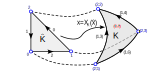
\includegraphics[width=1\linewidth]{figures/reference_mapping.pdf}
\end{center}
  \end{minipage}\\
Each component = (scalar-valued) finite-element function
$$
X \in \mathcal{W}_h^{\times} = \mathcal{W}_h \times \mathcal{W}_h \quad \text{vector function space}
$$
\end{frame}

%%%%%%%%%%%%%%%%%%%%%%%%%%%%%%%%%%%%%%%%%%%%%%%%%%%%%%%%%%%%%%%%%%

\begin{frame}
  \frametitle{Vector function spaces}
\textbf{Local degrees of freedom and basis functions of $\mathcal{W}^\times_h$}\\[1ex]
Vector-valued function $w=(w_0,w_1):\widehat{K}\rightarrow \mathbb{R}^2$\\
$\Rightarrow$ degrees of freedom $\lambda_{\ell^\times}^\times$ 
$$
\lambda^\times_{\ell^\times}(w) = \begin{cases} 
\lambda_{\frac{\ell^\times}{2}}(w_0) & \text{for $\ell^\times$ even}\\
\lambda_{\frac{\ell^\times-1}{2}}(w_1) & \text{for $\ell^\times$ odd}\\
\end{cases}
$$
Vector-valued nodal basis functions 
$$
\phi^\times_{\ell^\times}(x) = 
\begin{cases}
\begin{pmatrix}\phi_{\frac{\ell^\times}{2}}(x)\\0\end{pmatrix} & \text{for $\ell^\times$ even}\\[4ex]
\begin{pmatrix}0 \\\phi_{\frac{\ell^\times-1}{2}}(x)\end{pmatrix} & \text{for $\ell^\times$ odd}
\end{cases}
$$
$\Rightarrow$ $\lambda^{\times}_{\ell^\times}(\phi^\times_{k^\times})=\delta_{\ell^\times k^\times}$
\end{frame}

%%%%%%%%%%%%%%%%%%%%%%%%%%%%%%%%%%%%%%%%%%%%%%%%%%%%%%%%%%%%%%%%%%

\begin{frame}
  \frametitle{Tabulation of basis functions}
Given set of points $\boldsymbol{\zeta}:=\{\zeta^{(r)}\}_{r=0}^{n-1}$ $\Rightarrow$ $n \times \nu^\times \times 2$ matrix $T^\times$

$$
{\footnotesize
T^\times_{r\ell^\times a}(\boldsymbol{\zeta}) := (\phi^\times_{\ell^\times}(\zeta^{(r)}))_a = 
\begin{cases}
\phi_{\frac{\ell^\times}{2}}(\zeta^{(r)}) = T_{r,\frac{\ell^\times}{2}}& \text{if $\ell^\times$ even and $a=0$} \\
\phi_{\frac{\ell^\times-1}{2}}(\zeta^{(r)}) = T_{r,\frac{\ell^\times-1}{2}} & \text{if $\ell^\times$ odd and $a=1$} \\
0 & \text{otherwise}
\end{cases}}
$$

Derivatives $\Rightarrow$ $n \times \nu^\times \times 2\times 2$ matrix $T^{\times\partial}$ matrix

$$
{\footnotesize
T^{\times\partial}_{r\ell^\times ab}(\boldsymbol{\zeta}) := \frac{(\partial \phi^\times_{\ell^\times})_a}{\partial x_b}(\zeta^{(r)})  = \begin{cases}
\frac{\phi_{\frac{\ell^\times}{2}}}{\partial x_b}(\zeta^{(r)}) = T_{r,\frac{\ell^\times}{2},b}& \text{if $\ell^\times$ even, $a=0$} \\[2ex]
\frac{\partial\phi_{\frac{\ell^\times-1}{2}}}{\partial x_b}(\zeta^{(r)}) = T_{r,\frac{\ell^\times-1}{2},b} & \text{if $\ell^\times$ odd, $a=1$} \\[2ex]
0 & \text{otherwise}
\end{cases}}
$$
\end{frame}

%%%%%%%%%%%%%%%%%%%%%%%%%%%%%%%%%%%%%%%%%%%%%%%%%%%%%%%%%%%%%%%%%%

\begin{frame}
  \frametitle{Construction of global coordinates}
Evaluate global coordinate $X_K(\zeta^{(r)})$ at $\zeta^{(r)}\in\widehat{K}$
$$
(X_K(\zeta^{(r)}))_a = \sum_{\ell^\times} \overline{X}_{\ell^\times} \left(\phi_{\ell^\times}^\times(\zeta^{(r)})\right)_a = \sum_{\ell^\times} \overline{X}_{\ell^\times} T^\times_{r\ell^\times a} 
$$
\begin{itemize}
  \item global coordinate dof-vector $\vec{X}$
  \item local coordinate dof-vector $\overline{\boldsymbol{X}}$
\end{itemize}
$$
\overline{X}_{\ell^\times} = X_{\ell^\times_{\text{global}}(\alpha,\ell^\times)}.
$$
Global dof-index $\ell^\times_{\text{global}}(\alpha,\ell^\times)$ in cell with index $\alpha$
\end{frame}

%%%%%%%%%%%%%%%%%%%%%%%%%%%%%%%%%%%%%%%%%%%%%%%%%%%%%%%%%%%%%%%%%%

\begin{frame}[fragile]
  \frametitle{Implementation in Python}
Subclass abstract \lstinline{FiniteElement} class\\[1ex]
$\Rightarrow$ Class \lstinline{VectorElement(finiteelement)}
\begin{itemize}
\item method \lstinline{tabulate_dofs(fhat)}: tabulate $\left(\lambda_0(\widehat{f}),\lambda_1(\widehat{f}),\dots,\lambda_{\nu-1}(\widehat{f})\right)^\top\in \mathbb{R}^{\nu}$
for vector-valued $\widehat{f}$
\item method \lstinline{tabulate(zeta)}: tabulate\\$T^\times$ for points $\{\zeta^{(r)}\}_{r=0}^{n-1}$  (= array \lstinline{zeta} of shape $n\times 2$)
\item method \lstinline{tabulate_gradient(zeta)} tabulate\\$T^{\times\partial}$ for points $\{\zeta^{(r)}\}_{r=0}^{n-1}$
\end{itemize}
\textbf{Mesh geometry}\\[1ex]
Class \lstinline{Mesh} has property \lstinline{coordinates} = \lstinline{Function} on \lstinline{FunctionSpace} over \lstinline{VectorElements}
\end{frame}

%%%%%%%%%%%%%%%%%%%%%%%%%%%%%%%%%%%%%%%%%%%%%%%%%%%%%%%%%%%%%%%%%%

\section{Global assembly}

%%%%%%%%%%%%%%%%%%%%%%%%%%%%%%%%%%%%%%%%%%%%%%%%%%%%%%%%%%%%%%%%%%

\begin{frame}
  \tableofcontents[currentsection]
\end{frame}

%%%%%%%%%%%%%%%%%%%%%%%%%%%%%%%%%%%%%%%%%%%%%%%%%%%%%%%%%%%%%%%%%%


\begin{frame}
  \frametitle{Global assembly}
  Recall: need to solve
  $$
A^{(h)} \boldsymbol{u}^{(h)} = \boldsymbol{b}^{(h)}
$$
with \textbf{stiffness matrix} $A^{(h)}$
$$
A^{(h)}_{{\ell_{\text{global}}}{k_{\text{global}}}}:= a\left(\Phi^{(h)}_{k_{\text{global}}},\Phi^{(h)}_{\ell_{\text{global}}}\right).
$$
\textbf{right-hand-side vector} $\vec{b}^{(h)}$
$$
b^{(h)}_{\ell_{\text{global}}}:=b(\Phi^{(h)}_{\ell_{\text{global}}})
$$
$\Rightarrow$ dof-vector $\boldsymbol{u}^{(h)}$ $\Rightarrow$ finite element solution
$$
u_h(x) = \sum_{\ell=0}^{n-1} u^{(h)}_{\ell_{\text{global}}} \Phi^{(h)}_{\ell_{\text{global}}}(x)
$$
$\Rightarrow$ \textbf{global assembly} of $\vec{b}^{(h)}$ and $A^{(h)}$
\end{frame}

%%%%%%%%%%%%%%%%%%%%%%%%%%%%%%%%%%%%%%%%%%%%%%%%%%%%%%%%%%%%%%%%%%

\begin{frame}
  \frametitle{Assembly of right-hand-side}
  Recall $b(v) = \int_\Omega f(x)v(x)\;dx$ 
  $$
\begin{aligned}
\Rightarrow \quad b^{(h)}_{\ell_{\text{global}}} &= \int_\Omega f(x) \Phi_{\ell_{\text{global}}}(x)\;dx = \sum_{K\in \Omega_h} \int_K f(x) \Phi_{\ell_{\text{global}}}(x) \; dx\\
\end{aligned}
$$
global index $\ell_{\text{global}}=\ell_{\text{global}}(\alpha,\ell)$
\begin{itemize}
  \item index of cell $K$: $\alpha$
  \item local dof-index: $\ell$
\end{itemize}
{\footnotesize There can be $\alpha'\neq \alpha$, $\ell'\neq\ell$ such that $\ell_{\text{global}}(\alpha',\ell')=\ell_{\text{global}}(\alpha,\ell)$}\\[1ex]
\textbf{Change of variables $\int_{K}\;dx\rightarrow\int_{\widehat{K}}\;d\widehat{x}$:} 
$$
\begin{aligned}
b^{(h)}_{\ell_{\text{global}}} &= \sum_{K\in \Omega_h}\int_{\widehat{K}} \widehat{f}_K(\widehat{x}) \phi_\ell(\widehat{x})\;|\det{J}(\widehat{x})|\;d\widehat{x}
\end{aligned}
$$
\textbf{Pullback} of $f$ to the cell $K$: $\widehat{f}_K = f\circ X_K$:
$$
\widehat{f}_K(\widehat{x}) :=  f(x) = f(X_K(\widehat{x}))
\quad \text{for all $\widehat{x}\in\widehat{K}$}
$$
\end{frame}

%%%%%%%%%%%%%%%%%%%%%%%%%%%%%%%%%%%%%%%%%%%%%%%%%%%%%%%%%%%%%%%%%%

\begin{frame}
  \frametitle{Assembly of right-hand-side}
  \textbf{Numerical quadrature} and \textbf{tabulation}
$$
\begin{aligned}
b^{(h)}_{\ell_{\text{global}}} &\sum_{K\in \Omega_h}\int_{\widehat{K}} \widehat{f}_K(\widehat{x}) \phi_\ell(\widehat{x})\;|\det{J}(\widehat{x})|\;d\widehat{x}\\
&\approx \sum_{K\in \Omega_h} \sum_q w_q \widehat{f}_K(\xi^{(q)}) \phi_\ell(\xi^{(q)})\;|\det{J}(\xi^{(q)})|\\
&= \sum_{K\in \Omega_h} \sum_q w_q \widehat{f}_K(\xi^{(q)}) T_{q\ell}\;|\det{J}(\xi^{(q)})|.
\end{aligned}
$$
Evaluation of cell-local $\widehat{f}_K$ at quadrature points $\xi^{(q)}$\\
$\Rightarrow$ global coordinate $x_K^{(q)}=X_K(\xi^{(q)})$
$$
\widehat{f}_K(\xi^{(q)}) = f(x_K^{(q)}).
$$
\end{frame}

%%%%%%%%%%%%%%%%%%%%%%%%%%%%%%%%%%%%%%%%%%%%%%%%%%%%%%%%%%%%%%%%%%

\begin{frame}
  \frametitle{Assembly of right-hand-side}
  Expand $x_K$ in terms of vector-valued basis functions
$$
(x_K^{(q)})_a = (X_K(\xi^{(q)}))_a = \sum_{\ell^\times} (\phi^\times_{\ell^\times}(\xi^{(q)}))_a X_{\ell^\times_{\text{global}}} = \sum_{\ell^\times} T^\times_{q\ell^\times a} \overline{X}_{\ell^\times}
$$
global dof-index of coordinate field: $\ell^\times_{\text{global}}=\ell_{\text{global}}^\times(\alpha,\ell^\times)$\\
cell-local coordinate dof-vector $\overline{\boldsymbol{X}}$ with $\overline{X}_{\ell^\times} = X_{\ell_{\text{global}}^\times}$\\[2ex]
\textbf{Jacobian}
$$
\begin{aligned}
J_{ab}(\xi^{(q)}) &= \frac{\partial (x_K^{(q)})_a }{\partial x_b} = \frac{\partial (X_K)_a }{\partial x_b}(\xi^{(q)})\\
&= \sum_{\ell^\times} X_{\ell^\times_{\text{global}}} \frac{\partial (\phi^\times_{\ell^\times})_a }{\partial x_b}(\xi^{(q)})\\
&= \sum_{\ell^\times} \overline{X}_{\ell^\times} T^{\times\partial}_{q\ell^\times ab}
\end{aligned}
$$

\end{frame}

%%%%%%%%%%%%%%%%%%%%%%%%%%%%%%%%%%%%%%%%%%%%%%%%%%%%%%%%%%%%%%%%%%

\begin{frame}
  \frametitle{Assembly of right-hand-side}
  \begin{algorithmic}[1]    
\State{Initialise $\boldsymbol{b}^{(h)} \gets 0$}
\ForAll{cells $K$} 
  \State {Extract local coordinate dof-vector $\overline{\boldsymbol{X}}$ with $\overline{X}_{\ell^\times} = X_{\ell^\times_\text{global}}$}
  \ForAll{quadrature points $q$}
    \State{Compute the determinant $D_q$ of the Jacobian $J(\xi^{(q)})$ $$J_{ab}(\xi^{(q)}) = \sum_{\ell^\times} \overline{X}_{\ell^\times} T^{\times\partial}_{q\ell^\times ab}$$}
    \State{Compute $(x_K^{(q)})_a = \sum_{\ell^\times} T^\times_{q\ell^\times a} \overline{X}_{\ell^\times}$, $F_q =f(x_K^{(q)})$}
  \EndFor
  \State{Construct local $\boldsymbol{b}^{(h),\text{local}}$:
$b^{(h),\text{local}}_{\ell} = \sum_q w_q F_q T_{q\ell} D_q$}
\ForAll{local dof-indices $\ell$}
  \State{Increment $b_{\ell_{\text{global}}}^{(h)}\gets b_{\ell_{\text{global}}}^{(h)} + b^{(h),\text{local}}_\ell$}
\EndFor
\EndFor
  \end{algorithmic}
\end{frame}

%%%%%%%%%%%%%%%%%%%%%%%%%%%%%%%%%%%%%%%%%%%%%%%%%%%%%%%%%%%%%%%%%%

\begin{frame}
  \frametitle{Assembly of right-hand-side}
  \textbf{Illustration}
  \begin{center}
  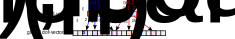
\includegraphics[width=\linewidth]{figures/global_assembly_rhs.pdf}
  \end{center}
  Global indices: $\ell_{\text{global}}=[2,4,8]$ (cell 1), $\ell_{\text{global}}=[8,11,16]$ (cell 2)\\
  $\Rightarrow$ Both cells contribute to the global vector entry $b^{(h)}_8$
\end{frame}

%%%%%%%%%%%%%%%%%%%%%%%%%%%%%%%%%%%%%%%%%%%%%%%%%%%%%%%%%%%%%%%%%%

\begin{frame}[fragile]
  \frametitle{Assembly of right-hand-side}
  \textbf{Implementation}\\[1ex]
  Summation $\sum_q w_q F_q T_{q\ell} D_q$ $\Rightarrow$ \lstinline{einsum()}\\
  \begin{lstlisting}
  np.einsum("q,ql,q,q->l", w_q, T, f_q, det_J)
  \end{lstlisting}
  Insertion of local vector $\boldsymbol{b}^{(h),\text{local}}$ into global vector $\boldsymbol{b}^{(h)}$\\
  $\Rightarrow$ \textbf{Slicing} notation {\footnotesize (avoid explicit looping)}
  \begin{lstlisting}
    ell_global = fs.local2global(alpha,range(ndof))
    b_h[ell_global] += b_h_local[:]
  \end{lstlisting}
\end{frame}

%%%%%%%%%%%%%%%%%%%%%%%%%%%%%%%%%%%%%%%%%%%%%%%%%%%%%%%%%%%%%%%%%%

\begin{frame}
  \frametitle{Assembly of stiffness matrix}
  $$
  {\footnotesize
\begin{aligned}
A^{(h)}_{\ell_{\text{global}},k_{\text{global}}} &= \int_\Omega \left(\kappa \nabla \Phi^{(h)}_{k_{\text{global}}}(x) \cdot\nabla\Phi^{(h)}_{\ell_{\text{global}}}(x)+\omega \Phi^{(h)}_{k_{\text{global}}}(x)\Phi^{(h)}_{\ell_{\text{global}}}(x)\right)dx\\
&= \sum_{K\in\Omega_h}\int_K \left(\kappa \nabla \Phi^{(h)}_{k_{\text{global}}}(x) \cdot\nabla\Phi^{(h)}_{\ell_{\text{global}}}(x)+\omega \Phi^{(h)}_{k_{\text{global}}}(x)\Phi^{(h)}_{\ell_{\text{global}}}(x)\right)dx
\end{aligned}}
$$
\textbf{Change of variables $\int_{K}\;dx\rightarrow\int_{\widehat{K}}\;d\widehat{x}$:} 
$$
\begin{aligned}
\Phi^{(h)}_{\ell_{\text{global}}}(x) &= \phi_\ell(\widehat{x})\\
\nabla \Phi^{(h)}_{\ell_{\text{global}}}(x) &= J^{-\top}(\widehat{x}) \widehat{\nabla}\phi_\ell(\widehat{x})
\end{aligned}
$$
$$
{\footnotesize
\begin{aligned}
A^{(h)}_{\ell_{\text{global}},k_{\text{global}}} &= \sum_{K\in \Omega_h}\int_K \Big(\kappa J^{-\top}(\widehat{x}) \widehat{\nabla} \phi_k (\widehat{x})\cdot J^{-\top}(\widehat{x})\widehat{\nabla}\phi_\ell(\widehat{x})+ \omega\phi_k(\widehat{x})\phi_\ell(\widehat{x})\Big)\cdot\\[-2ex]
&\hspace{7cm}\cdot|\det{J}(\widehat{x})|d\widehat{x}
\end{aligned}}
$$
\end{frame}

%%%%%%%%%%%%%%%%%%%%%%%%%%%%%%%%%%%%%%%%%%%%%%%%%%%%%%%%%%%%%%%%%%

\begin{frame}
  \frametitle{Assembly of stiffness matrix}
  \textbf{Numerical quadrature} and \textbf{tabulation}
  $$
  {\footnotesize
\begin{aligned}
A^{(h)}_{\ell_{\text{global}},k_{\text{global}}} &= \sum_{K\in \Omega_h}\int_K \Big(\kappa J^{-\top}(\widehat{x}) \widehat{\nabla} \phi_k (\widehat{x})\cdot J^{-\top}(\widehat{x})\widehat{\nabla}\phi_\ell(\widehat{x})+ \omega\phi_k(\widehat{x})\phi_\ell(\widehat{x})\Big)\cdot\\[-2ex]
&\hspace{7cm}\cdot|\det{J}(\widehat{x})|d\widehat{x}
\\
&\approx \sum_{K\in \Omega_h}\int_K  w_q \left(\kappa \widehat{\nabla} \phi_k(\xi^{(q)})(J^{\top}(\xi^{(q)}) J(\xi^{(q)}))^{-1}\phi_\ell(\xi^{(q)}) + \omega\phi_k(\xi^{(q)})\phi_\ell(\xi^{(q)})\right)|\det{J}(\xi^{(q)})| \\
&= \sum_{K\in \Omega_h} \sum_q w_q  \left(\kappa T^\partial_{qka}(J^{(-2)}_q)_{ab} T^\partial_{q\ell b} +\omega T_{qk}T_{q\ell}\right)|\det{J}(\xi^{(q)})|
\end{aligned}}
$$
with $2\times 2$ matrix
$$
J^{(-2)}_{q} =  \left(J^{\top}(\xi^{(q)}) J(\xi^{(q)})\right)^{-1}
$$
\end{frame}

%%%%%%%%%%%%%%%%%%%%%%%%%%%%%%%%%%%%%%%%%%%%%%%%%%%%%%%%%%%%%%%%%%

\begin{frame}
  \frametitle{Assembly of stiffness matrix}
  {\footnotesize
  \begin{algorithmic}[1]
  \State{Initialise $A^{(h)} \gets 0$}
  \ForAll{all cells $K$}
    \State{Extract coordinate dof-vector $\overline{\boldsymbol{X}}$ with $\overline{X}_{\ell^\times} = X_{\ell^\times_\text{global}(\alpha,\ell^\times)}$}
    \ForAll{all quadrature points $q$}
      \State{Compute Jacobian $J(\xi^{(q)})$: $J_{qab} = J_{ab}(\xi^{(q)}) = \sum_{\ell^\times} \overline{X}_{\ell^\times} T^{\times\partial}_{q\ell^{\times}ab}$}
      \State{Compute determinant $D_q$ of $J(\xi^{(q)})$}
      \State{Compute matrix $J^{(2)}_q = J^{\top}(\xi^{(q)}) J(\xi^{(q)})$ with $J^{(2)}_{qab} = \sum_{c} J_{qca}J_{qcb}$}
      \State{Invert $J^{(2)}_q$ to obtain $J^{(-2)}_{q} = \left(J^{(2)}_q\right)^{-1}$}
    \EndFor
    \State{Construct the local stiffness matrix $A^{(h),\text{local}}$ with
$$A^{(h),\text{local}}_{\ell k} = \kappa \sum_{qab}w_q  T^\partial_{qka}(J^{(-2)}_q)_{ab} T^\partial_{q\ell b} D_q + \omega \sum_{q} w_q  T_{qk}T_{q\ell} D_q$$}
    \ForAll{local dof-indices $\ell$}
      \ForAll{local dof-indices $k$}
        \State{Increment $A^{(h)}_{\ell_{\text{global}},k_{\text{global}}}\gets A^{(h)}_{\ell_{\text{global}},k_{\text{global}}} + A^{(h),\text{local}}_{\ell k}$}
      \EndFor
    \EndFor
    \EndFor
  \end{algorithmic}}
\end{frame}

%%%%%%%%%%%%%%%%%%%%%%%%%%%%%%%%%%%%%%%%%%%%%%%%%%%%%%%%%%%%%%%%%%

\begin{frame}
  \frametitle{Assembly of stiffness matrix}
  \textbf{Illustration}
  \begin{center}
  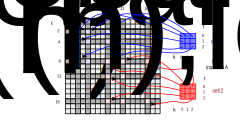
\includegraphics[width=\linewidth]{figures/global_assembly_stiffness_matrix.pdf}
  \end{center}
Global indices $\ell_{\text{global}}=[2,4,8]$ (cell 1), $\ell_{\text{global}}=[8,11,16]$ (cell 2)\\
$\Rightarrow$ both cells contribute to global matrix entry $A^{(h)}_{8,8}$
\end{frame}

%%%%%%%%%%%%%%%%%%%%%%%%%%%%%%%%%%%%%%%%%%%%%%%%%%%%%%%%%%%%%%%%%%

\begin{frame}[fragile]
  \frametitle{Assembly of stiffness matrix}
  \textbf{Implementation}\\[1ex]
  Summation
  \begin{itemize}
  \item $\sum_{c} J_{qca}J_{qcb}$
  \item $\sum_{qab}w_q  T^\partial_{q\ell a}(J^{(2)}_q)_{ab} T^\partial_{qkb} D_q$
  \item $\sum_{q}w_q  T_{q\ell}T_{qk} D_q$
  \end{itemize}
  $\Rightarrow$ \lstinline{einsum()}
  \begin{lstlisting}
np.einsum("qca,qcb->qab", J, J)
np.einsum("q,qka,qab,qlb,q->lk",
          w_q,T_grad,JT_J_inv,T_grad,D_q)
np.einsum("q,qk,ql,q->lk",w_q,T,T,D_q)
  \end{lstlisting}
\end{frame}

%%%%%%%%%%%%%%%%%%%%%%%%%%%%%%%%%%%%%%%%%%%%%%%%%%%%%%%%%%%%%%%%%%

\begin{frame}[fragile]
  \frametitle{Assembly of stiffness matrix}
Insert entries of local $A^{(h),\text{local}}$ into global $A^{(h)}$:\\[1ex]
\textbf{Naive attempt}
\begin{lstlisting}
ell_global = fs.local2global(i,range(ndof))
A_h[ell_global, ell_global] += A_h_local[:,:]
\end{lstlisting}
\textbf{Correct implementation}\\
$\ell_{\text{global}}\times \ell_{\text{global}}$ = \lstinline{np.ix_(ell_global, ell_global)}
\begin{lstlisting}
A_h[np.ix_(ell_global, ell_global)] += A_h_local[:,:]
\end{lstlisting}
\end{frame}

%%%%%%%%%%%%%%%%%%%%%%%%%%%%%%%%%%%%%%%%%%%%%%%%%%%%%%%%%%%%%%%%%%

\section{Numerical experiments}

%%%%%%%%%%%%%%%%%%%%%%%%%%%%%%%%%%%%%%%%%%%%%%%%%%%%%%%%%%%%%%%%%%

\begin{frame}
  \tableofcontents[currentsection]
\end{frame}

%%%%%%%%%%%%%%%%%%%%%%%%%%%%%%%%%%%%%%%%%%%%%%%%%%%%%%%%%%%%%%%%%%

\begin{frame}[fragile]
  \frametitle{Numerical experiments}
Diffusion-reaction equation
  $$
\begin{aligned}
  -\nabla \cdot (\kappa \nabla  u(x)) + \omega\; u(x) &= f(x) \qquad \text{for $x\in \Omega=[0,1]\times[0,1]$}\\
  \kappa\; n\cdot \nabla u(x)&=0 \qquad\quad \text{for $x\in\partial \Omega$}
\end{aligned}
$$
\textbf{Manufactured solution}
$$
\begin{aligned}
u(x) &= \cos(\pi s_0 x_0) \cos(\pi s_1 x_1)\\
f(x) &= \left((s_0^2 + s_1^2) \pi^2 \kappa + \omega\right)u(x)
\end{aligned}
$$
Numerical parameters
\begin{itemize}
\item $\kappa = 0.9$
\item $\omega = 0.4$
\item $s_0=2$, $s_1=4$
\end{itemize}
\end{frame}

%%%%%%%%%%%%%%%%%%%%%%%%%%%%%%%%%%%%%%%%%%%%%%%%%%%%%%%%%%%%%%%%%%

\begin{frame}[fragile]
  \frametitle{Implementation}
  Piecewise linear function space on $[0,1]\times[0,1]$
  \begin{lstlisting}
element = LinearElement()
mesh = rectangle_mesh(Lx=1.0, Ly=1.0, nref=nref)
fs = FunctionSpace(mesh, element)
  \end{lstlisting}
  \textbf{Assemble vector} $\boldsymbol{b}^{(h)}$ and \textbf{stiffness matrix} $A^{(h)}$:
  \begin{lstlisting}
quad = GaussLegendreQuadratureReferenceTriangle(2)
b_h = CoFunction(fs)
assemble_rhs(f, b_h, quad)
A_h = assemble_lhs(fs, quad, kappa, omega)
  \end{lstlisting}
  \textbf{Solve linear system}
  \begin{lstlisting}
u_h.data[:] = np.linalg.solve(A_h, b_h.data)
u_h = Function(fs)
  \end{lstlisting}
\end{frame}

%%%%%%%%%%%%%%%%%%%%%%%%%%%%%%%%%%%%%%%%%%%%%%%%%%%%%%%%%%%%%%%%%%

\begin{frame}[fragile]
  \frametitle{Numerical experiments}
  \textbf{Visualisation of solution and error}
  \begin{lstlisting}
X, Y, Z = grid_function(u_h,nx=100,ny=100)
  \end{lstlisting}
   Evaluate function $u_h$ at points of structured grid
$$
x_{i,j} = \begin{pmatrix}
x^{(0)}_0+H_x i \\ x^{(0)}_1 + H_y j
\end{pmatrix}\in\mathbb{R}^2
\qquad\text{{\footnotesize$i=0,1,\dots,n_x$, $j=0,1,\dots,n_y$}}
$$
\begin{itemize}
\item $x$- coordinates of grid vertices: $X_{i,j} = x^{(0)}_0+H_x i$
\item $y$- coordiantes of grid vertices: $Y_{i,j} = x^{(0)}_1+H_y j$
\item values of function $u_h$ at vertices: $Z_{i,j} = u_h(x_{i,j})$
\end{itemize}
Plot with \lstinline{contourf()}
\begin{lstlisting}
from matplotlib import pyplot as plt
X, Y, Z = grid_function(u_h)
plt.contourf(X, Y, Z)
\end{lstlisting}
\end{frame}

%%%%%%%%%%%%%%%%%%%%%%%%%%%%%%%%%%%%%%%%%%%%%%%%%%%%%%%%%%%%%%%%%%

\begin{frame}[fragile]
  \frametitle{Numerical experiments}
Compare numerical solution $u_h(x)$ to exact solution

$$
u_{\text{exact}}(x) = \cos(2\pi x_0)\cos(4\pi x_1)
$$
\begin{lstlisting}
Z_exact = np.cos(2*np.pi*X)*np.cos(4*np.pi*Y)
plt.contourf(X, Y, Z-Z_exact)
\end{lstlisting}

\begin{center}
\includegraphics[width=\linewidth]{figures/solution_linear.png}
\end{center}
\end{frame}

%%%%%%%%%%%%%%%%%%%%%%%%%%%%%%%%%%%%%%%%%%%%%%%%%%%%%%%%%%%%%%%%%%

\begin{frame}[fragile]
  \frametitle{Numerical experiments}
\begin{center}
{\tiny piecewise linear elements ($p=1$)}\\
\includegraphics[width=0.75\linewidth]{figures/solution_linear.png}\\
{\tiny piecewise cubic elements ($p=3$)}\\
\includegraphics[width=0.75\linewidth]{figures/solution_cubic.png}
\end{center}
\end{frame}

%%%%%%%%%%%%%%%%%%%%%%%%%%%%%%%%%%%%%%%%%%%%%%%%%%%%%%%%%%%%%%%%%%

\begin{frame}[fragile]
  \frametitle{Performance analysis}
  Increased resolution $\Rightarrow$
  \begin{itemize}
  \item Improved accuracy
  \item Longer runtime
  \end{itemize}
  Measure time spent in
  \begin{itemize}
  \item Assembly of $\boldsymbol{b}^{(h)}$ with \lstinline{assemble_rhs()}
  \item Assembly of $A^{(h)}$ with \lstinline{assemble_lhs()}
  \item Solution of the linear system $A^{(h)}\boldsymbol{u}^{(h)} = \boldsymbol{b}^{(h)}$ with \lstinline{np.linalg.solve()}
  \end{itemize}
Use \textbf{decorator}
\begin{lstlisting}
from fem.utilities import measure_time
with measure_time("assemble stiffness matrix"):
    A_h = assemble_lhs(fs, quad, kappa, omega)
\end{lstlisting}
\end{frame}

%%%%%%%%%%%%%%%%%%%%%%%%%%%%%%%%%%%%%%%%%%%%%%%%%%%%%%%%%%%%%%%%%%

\begin{frame}[fragile]
  \frametitle{Performance analysis}
  \begin{center}
  \includegraphics[width=\linewidth]{figures/runtime_dense.pdf}
  \end{center}
\begin{itemize}
\item $L_2$ error decreases $\|u_h-u_{\text{exact}}\|_{L_2(\Omega)}\propto h^2\propto n_{\text{dof}}^{-1}$
\item Assembly of $A^{(h)}$, $\vec{b}^{(h)}$: $T_{\text{assembly}}\propto n_{\text{dof}}\propto n_{\text{cell}}$
\item Solution of $A^{(h)}\boldsymbol{u}^{(h)}=\boldsymbol{b}^{(h)}$: $T_{\text{solve}}\propto n_{\text{dof}}^3$
\end{itemize}
\end{frame}

%%%%%%%%%%%%%%%%%%%%%%%%%%%%%%%%%%%%%%%%%%%%%%%%%%%%%%%%%%%%%%%%%%

\begin{frame}[fragile]
  \frametitle{Performance analysis}
  \textbf{Solve time}\\[1ex]
  $$
  T_{\text{solve}}\propto n_{\text{dof}}^3
  $$
  Extrapolating
  \begin{center}
    \renewcommand{\arraystretch}{1.5}
    \begin{tabular}{ccc}
      \hline
      $n_{\text{dof}}$ & $\|u_h-u_{\text{exact}}\|_{L_2(\Omega)}$ & $T_{\text{solve}}$\\\hline\hline
      $16641$ & $7.8\cdot 10^{-4}$ & $48\text{s}$\\
      $1.3\cdot 10^6$ & $10^{-5}$ & $264\text{days}$\\
      \hline
    \end{tabular}
  \end{center}
  \begin{itemize}
  \item Why is this so expensive?
  \item How can we improve this?
  \end{itemize}
\end{frame}

%%%%%%%%%%%%%%%%%%%%%%%%%%%%%%%%%%%%%%%%%%%%%%%%%%%%%%%%%%%%%%%%%%

\begin{frame}[fragile]
  \frametitle{Complexity analysis}
  \textbf{Solve linear system}
  $$
  A\boldsymbol{u}=\boldsymbol{b}$$
  \begin{itemize}
    \item $\boldsymbol{u}, \boldsymbol{b}\in\mathbb{R}^n$
    \item $A$: $n\times n$ matrix
  \end{itemize}
  \textbf{Gaussian elimination}\footnote{$LU$ factorisation} with \lstinline{numpy.linalg.solve()}\\[1ex]
  Example: $5\times 5$ system
$$
    \underbrace{
      \begin{pmatrix}
\textcolor{red}{1.096} & \textcolor{black}{0.3391} & \textcolor{black}{0.0632} & \textcolor{black}{0.0555} & \textcolor{black}{0.2176}\\
\textcolor{green}{0.3687} & \textcolor{blue}{1.311} & \textcolor{blue}{0.0862} & \textcolor{blue}{0.3232} & \textcolor{blue}{0.0849}\\
\textcolor{green}{0.2743} & \textcolor{blue}{0.2277} & \textcolor{blue}{1.15} & \textcolor{blue}{0.0511} & \textcolor{blue}{0.2343}\\
\textcolor{green}{0.1019} & \textcolor{blue}{0.0976} & \textcolor{blue}{0.0082} & \textcolor{blue}{1.285} & \textcolor{blue}{0.3212}\\
\textcolor{green}{0.3629} & \textcolor{blue}{0.2885} & \textcolor{blue}{0.012} & \textcolor{blue}{0.1747} & \textcolor{blue}{1.145}
\end{pmatrix}}_{=A}
\underbrace{\begin{pmatrix}
u_0 \\ u_1 \\ u_2 \\ u_3 \\ u_4
\end{pmatrix}}_{=\boldsymbol{u}}
=
\underbrace{
  \begin{pmatrix}
\textcolor{black}{0.23}\\
\textcolor{blue}{0.51}\\
\textcolor{blue}{0.29}\\
\textcolor{blue}{0.82}\\
\textcolor{blue}{0.98}
\end{pmatrix}}_{=\boldsymbol{b}}
$$
\end{frame}

%%%%%%%%%%%%%%%%%%%%%%%%%%%%%%%%%%%%%%%%%%%%%%%%%%%%%%%%%%%%%%%%%%

\begin{frame}[fragile]
  \frametitle{Complexity analysis}
  Transformation into equivalent \textbf{upper triangular system}\\[1ex]
Eliminate all entries below the diagonal in the first row
\begin{algorithmic}[1]
\ForAll{matrix rows $i=1,2,\dots,n-1$}
\ForAll {$j=1,2,\dots,n-1$}
\State {$\textcolor{blue}{A_{ij}} \mapsto \textcolor{blue}{A_{ij}} - \textcolor{green}A_{i0}/\textcolor{red}{A_{00}}\cdot A_{0j}$}\Comment{{\footnotesize$\textcolor{blue}{\text{row}_i}\mapsto \textcolor{blue}{\text{row}_i}-\textcolor{green}{A_{i0}}/\textcolor{red}{A_{00}}\cdot\textcolor{blue}{\text{row}_0}$}}
\EndFor
\State{$b_i \mapsto b_i - \textcolor{green}{A_{i0}}/\textcolor{red}{A_{00}}\cdot b_0$} \Comment{\footnotesize Modify right-hand-side $\boldsymbol{b}$}
\EndFor
\end{algorithmic}

$$
      \begin{pmatrix}
\textcolor{red}{1.096} & \textcolor{black}{0.3391} & \textcolor{black}{0.0632} & \textcolor{black}{0.0555} & \textcolor{black}{0.2176}\\
\textcolor{green}{0.3687} & \textcolor{blue}{1.311} & \textcolor{blue}{0.0862} & \textcolor{blue}{0.3232} & \textcolor{blue}{0.0849}\\
\textcolor{green}{0.2743} & \textcolor{blue}{0.2277} & \textcolor{blue}{1.15} & \textcolor{blue}{0.0511} & \textcolor{blue}{0.2343}\\
\textcolor{green}{0.1019} & \textcolor{blue}{0.0976} & \textcolor{blue}{0.0082} & \textcolor{blue}{1.285} & \textcolor{blue}{0.3212}\\
\textcolor{green}{0.3629} & \textcolor{blue}{0.2885} & \textcolor{blue}{0.012} & \textcolor{blue}{0.1747} & \textcolor{blue}{1.145}
\end{pmatrix}
\begin{pmatrix}
u_0 \\ u_1 \\ u_2 \\ u_3 \\ u_4
\end{pmatrix}
=
  \begin{pmatrix}
\textcolor{black}{0.23}\\
\textcolor{blue}{0.51}\\
\textcolor{blue}{0.29}\\
\textcolor{blue}{0.82}\\
\textcolor{blue}{0.98}
\end{pmatrix}
$$
\end{frame}

%%%%%%%%%%%%%%%%%%%%%%%%%%%%%%%%%%%%%%%%%%%%%%%%%%%%%%%%%%%%%%%%%%

\begin{frame}[fragile]
  \frametitle{Complexity analysis}
$$
{\footnotesize
\begin{aligned}
      \begin{pmatrix}
\textcolor{red}{1.096} & \textcolor{black}{0.3391} & \textcolor{black}{0.0632} & \textcolor{black}{0.0555} & \textcolor{black}{0.2176}\\
\textcolor{green}{0.3687} & \textcolor{blue}{1.311} & \textcolor{blue}{0.0862} & \textcolor{blue}{0.3232} & \textcolor{blue}{0.0849}\\
\textcolor{green}{0.2743} & \textcolor{blue}{0.2277} & \textcolor{blue}{1.15} & \textcolor{blue}{0.0511} & \textcolor{blue}{0.2343}\\
\textcolor{green}{0.1019} & \textcolor{blue}{0.0976} & \textcolor{blue}{0.0082} & \textcolor{blue}{1.285} & \textcolor{blue}{0.3212}\\
\textcolor{green}{0.3629} & \textcolor{blue}{0.2885} & \textcolor{blue}{0.012} & \textcolor{blue}{0.1747} & \textcolor{blue}{1.145}
\end{pmatrix}
\begin{pmatrix}
u_0 \\ u_1 \\ u_2 \\ u_3 \\ u_4
\end{pmatrix}
&=
\begin{pmatrix}
\textcolor{black}{0.23}\\
\textcolor{blue}{0.51}\\
\textcolor{blue}{0.29}\\
\textcolor{blue}{0.82}\\
\textcolor{blue}{0.98}
\end{pmatrix}\\[2ex]
&\downarrow\\[2ex]
    \begin{pmatrix}
1.096 & 0.3391 & 0.0632 & 0.0555 & 0.2176\\
\textcolor{lightgray}{0} & \textcolor{red}{1.197} & \textcolor{black}{0.06495} & \textcolor{black}{0.3045} & \textcolor{black}{0.01172}\\
\textcolor{lightgray}{0} & \textcolor{green}{0.1429} & \textcolor{blue}{1.134} & \textcolor{blue}{0.03721} & \textcolor{blue}{0.1799}\\
\textcolor{lightgray}{0} & \textcolor{green}{0.06608} & \textcolor{blue}{0.002326} & \textcolor{blue}{1.28} & \textcolor{blue}{0.301}\\
\textcolor{lightgray}{0} & \textcolor{green}{0.1763} & \textcolor{blue}{-0.008921} & \textcolor{blue}{0.1563} & \textcolor{blue}{1.073}
\end{pmatrix}
\begin{pmatrix}
u_0 \\ u_1 \\ u_2 \\ u_3 \\ u_4
\end{pmatrix}
    &=  \begin{pmatrix}
0.23\\
\textcolor{black}{0.4326}\\
\textcolor{blue}{0.2325}\\
\textcolor{blue}{0.7986}\\
\textcolor{blue}{0.9039}
\end{pmatrix}
\end{aligned}
}
$$
NB: first row of $A$ and $b_0$ remain unchanged
\end{frame}

%%%%%%%%%%%%%%%%%%%%%%%%%%%%%%%%%%%%%%%%%%%%%%%%%%%%%%%%%%%%%%%%%%

\begin{frame}[fragile]
  \frametitle{Complexity analysis}
  For rows $i=1,2,\dots,n-1$:
\begin{itemize}
\item compute $\rho_i = -A_{i0}/A_{00}$\\
{}\qquad $\Rightarrow$ $\boldsymbol{1}$ \textbf{division}
\item scale first row by $\rho_i$, scaled first row to row $i$\\
{}\qquad $\Rightarrow$  $\boldsymbol{n-1}$ \textbf{multiplications} and $\boldsymbol{n-1}$ \textbf{additions}\footnote{can ignore the first entry which will be set to zero by construction}
\item update $b_i \gets b_i - \rho_i \cdot b_0$\\
{}\qquad $\Rightarrow$ $\boldsymbol{1}$ \textbf{multiplication} and $\boldsymbol{1}$ \textbf{subtraction}
\end{itemize}
Total number of operations for all $n-1$ rows:
$$
(3+2(n-1))(n-1)
$$
\end{frame}

%%%%%%%%%%%%%%%%%%%%%%%%%%%%%%%%%%%%%%%%%%%%%%%%%%%%%%%%%%%%%%%%%%

\begin{frame}[fragile]
  \frametitle{Complexity analysis}
  \textbf{Repeat} for $(n-1)\times (n-1)$ matrix in lower right corner\\
  $\Rightarrow$ zero out all entries below diagonal in 2nd column
$$
  {\footnotesize
  \begin{aligned}
    \begin{pmatrix}
1.096 & 0.3391 & 0.0632 & 0.0555 & 0.2176\\
\textcolor{lightgray}{0} & \textcolor{red}{1.197} & \textcolor{black}{0.06495} & \textcolor{black}{0.3045} & \textcolor{black}{0.01172}\\
\textcolor{lightgray}{0} & \textcolor{green}{0.1429} & \textcolor{blue}{1.134} & \textcolor{blue}{0.03721} & \textcolor{blue}{0.1799}\\
\textcolor{lightgray}{0} & \textcolor{green}{0.06608} & \textcolor{blue}{0.002326} & \textcolor{blue}{1.28} & \textcolor{blue}{0.301}\\
\textcolor{lightgray}{0} & \textcolor{green}{0.1763} & \textcolor{blue}{-0.008921} & \textcolor{blue}{0.1563} & \textcolor{blue}{1.073}
\end{pmatrix}
\begin{pmatrix}
u_0 \\ u_1 \\ u_2 \\ u_3 \\ u_4
\end{pmatrix}
    &=  \begin{pmatrix}
0.23\\
\textcolor{black}{0.4326}\\
\textcolor{blue}{0.2325}\\
\textcolor{blue}{0.7986}\\
\textcolor{blue}{0.9039}
\end{pmatrix}\\[2ex]
&\downarrow\\[2ex]
    \begin{pmatrix}
1.096 & 0.3391 & 0.0632 & 0.0555 & 0.2176\\
\textcolor{lightgray}{0} & 1.197 & 0.06495 & 0.3045 & 0.01172\\
\textcolor{lightgray}{0} & \textcolor{lightgray}{0} & \textcolor{red}{1.127} & \textcolor{black}{0.0008768} & \textcolor{black}{0.1785}\\
\textcolor{lightgray}{0} & \textcolor{lightgray}{0} & \textcolor{green}{-0.001259} & \textcolor{blue}{1.263} & \textcolor{blue}{0.3003}\\
\textcolor{lightgray}{0} & \textcolor{lightgray}{0} & \textcolor{green}{-0.01848} & \textcolor{blue}{0.1115} & \textcolor{blue}{1.071}
\end{pmatrix}
\begin{pmatrix}
u_0 \\ u_1 \\ u_2 \\ u_3 \\ u_4
\end{pmatrix}
&=
    \begin{pmatrix}
0.23\\
0.4326\\
\textcolor{black}{0.1808}\\
\textcolor{blue}{0.7747}\\
\textcolor{blue}{0.8402}
\end{pmatrix}
\end{aligned}}
$$
NB: first \textbf{two} rows not modified
\end{frame}

%%%%%%%%%%%%%%%%%%%%%%%%%%%%%%%%%%%%%%%%%%%%%%%%%%%%%%%%%%%%%%%%%%

\begin{frame}[fragile]
  \frametitle{Complexity analysis}
  \textbf{Repeat} for $(n-2)\times (n-2)$ matrix in lower right corner\\
  $\Rightarrow$ zero out all entries below diagonal in 3rd column
  $$
{\footnotesize
\begin{aligned}
    \begin{pmatrix}
1.096 & 0.3391 & 0.0632 & 0.0555 & 0.2176\\
\textcolor{lightgray}{0} & 1.197 & 0.06495 & 0.3045 & 0.01172\\
\textcolor{lightgray}{0} & \textcolor{lightgray}{0} & \textcolor{red}{1.127} & \textcolor{black}{0.0008768} & \textcolor{black}{0.1785}\\
\textcolor{lightgray}{0} & \textcolor{lightgray}{0} & \textcolor{green}{-0.001259} & \textcolor{blue}{1.263} & \textcolor{blue}{0.3003}\\
\textcolor{lightgray}{0} & \textcolor{lightgray}{0} & \textcolor{green}{-0.01848} & \textcolor{blue}{0.1115} & \textcolor{blue}{1.071}
\end{pmatrix}
\begin{pmatrix}
u_0 \\ u_1 \\ u_2 \\ u_3 \\ u_4
\end{pmatrix}
&=
    \begin{pmatrix}
0.23\\
0.4326\\
\textcolor{black}{0.1808}\\
\textcolor{blue}{0.7747}\\
\textcolor{blue}{0.8402}
\end{pmatrix}\\[2ex]
&\downarrow\\[2ex]
    \begin{pmatrix}
1.096 & 0.3391 & 0.0632 & 0.0555 & 0.2176\\
\textcolor{lightgray}{0} & 1.197 & 0.06495 & 0.3045 & 0.01172\\
\textcolor{lightgray}{0} & \textcolor{lightgray}{0} & 1.127 & 0.0008768 & 0.1785\\
\textcolor{lightgray}{0} & \textcolor{lightgray}{0} & \textcolor{lightgray}{0} & \textcolor{red}{1.263} & \textcolor{black}{0.3005}\\
\textcolor{lightgray}{0} & \textcolor{lightgray}{0} & \textcolor{lightgray}{0} & \textcolor{green}{0.1115} & \textcolor{blue}{1.074}
\end{pmatrix}
\begin{pmatrix}
u_0 \\ u_1 \\ u_2 \\ u_3 \\ u_4
\end{pmatrix}
&=
\begin{pmatrix}
0.23\\
0.4326\\
0.1808\\
\textcolor{black}{0.7749}\\
\textcolor{blue}{0.8431}
\end{pmatrix}
\end{aligned}}
$$
NB: first \textbf{three} rows not modified
\end{frame}

%%%%%%%%%%%%%%%%%%%%%%%%%%%%%%%%%%%%%%%%%%%%%%%%%%%%%%%%%%%%%%%%%%

\begin{frame}[fragile]
  \frametitle{Complexity analysis}
  \textbf{Repeat} for $2\times 2$ matrix in lower right corner\\
  $\Rightarrow$ zero out all entries below diagonal in 4th column
  $$
  {\footnotesize
\begin{aligned}
    \begin{pmatrix}
1.096 & 0.3391 & 0.0632 & 0.0555 & 0.2176\\
\textcolor{lightgray}{0} & 1.197 & 0.06495 & 0.3045 & 0.01172\\
\textcolor{lightgray}{0} & \textcolor{lightgray}{0} & 1.127 & 0.0008768 & 0.1785\\
\textcolor{lightgray}{0} & \textcolor{lightgray}{0} & \textcolor{lightgray}{0} & \textcolor{red}{1.263} & \textcolor{black}{0.3005}\\
\textcolor{lightgray}{0} & \textcolor{lightgray}{0} & \textcolor{lightgray}{0} & \textcolor{green}{0.1115} & \textcolor{blue}{1.074}
\end{pmatrix}
\begin{pmatrix}
u_0 \\ u_1 \\ u_2 \\ u_3 \\ u_4
\end{pmatrix}
&=
\begin{pmatrix}
0.23\\
0.4326\\
0.1808\\
\textcolor{black}{0.7749}\\
\textcolor{blue}{0.8431}
\end{pmatrix}\\[2ex]
&\downarrow\\[2ex]
\begin{pmatrix}
1.096 & 0.3391 & 0.0632 & 0.0555 & 0.2176\\
\textcolor{lightgray}{0} & 1.197 & 0.06495 & 0.3045 & 0.01172\\
\textcolor{lightgray}{0} & \textcolor{lightgray}{0} & 1.127 & 0.0008768 & 0.1785\\
\textcolor{lightgray}{0} & \textcolor{lightgray}{0} & \textcolor{lightgray}{0} & 1.263 & 0.3005\\
\textcolor{lightgray}{0} & \textcolor{lightgray}{0} & \textcolor{lightgray}{0} & \textcolor{lightgray}{0} & 1.047
\end{pmatrix}
\begin{pmatrix}
u_0 \\ u_1 \\ u_2 \\ u_3 \\ u_4
\end{pmatrix}
&=
\begin{pmatrix}
0.23\\
0.4326\\
0.1808\\
0.7749\\
0.7747
\end{pmatrix}
\end{aligned}}
$$
NB: first \textbf{four} rows not modified
\end{frame}

%%%%%%%%%%%%%%%%%%%%%%%%%%%%%%%%%%%%%%%%%%%%%%%%%%%%%%%%%%%%%%%%%%

\begin{frame}[fragile]
  \frametitle{Complexity analysis}
  \textbf{Total computational cost}\\[1ex]
  Sum number of arithmetic operations for all $n-1$ steps:
$$
\begin{aligned}
E_{\text{transform}}(n) &= (3+2(n-1))(n-1)\\
&\quad+\;\; (3+2(n-2))(n-2)\\
&\quad+\;\; (3+2(n-3))(n-3)\\
&\quad+\;\; \dots +(3+2\cdot 1)\cdot 1\\
&= \sum_{k=1}^{n-1} (3+2k)k\\
&= \frac{3}{2} n(n-1) + \frac{1}{3} n(n-1)(2n-1)\\
&= \frac{2}{3} n^3 + \mathcal{O}(n^2)
\end{aligned}
$$
\end{frame}

%%%%%%%%%%%%%%%%%%%%%%%%%%%%%%%%%%%%%%%%%%%%%%%%%%%%%%%%%%%%%%%%%%

\begin{frame}[fragile]
  \frametitle{Complexity analysis}
  \textbf{Solution of upper triangular system}
  $$
  {\footnotesize
\begin{aligned}
\begin{pmatrix}
1.096 & 0.3391 & 0.0632 & 0.0555 & 0.2176\\
\textcolor{lightgray}{0} & 1.197 & 0.06495 & 0.3045 & 0.01172\\
\textcolor{lightgray}{0} & \textcolor{lightgray}{0} & 1.127 & 0.0008768 & 0.1785\\
\textcolor{lightgray}{0} & \textcolor{lightgray}{0} & \textcolor{lightgray}{0} & 1.263 & 0.3005\\
\textcolor{lightgray}{0} & \textcolor{lightgray}{0} & \textcolor{lightgray}{0} & \textcolor{lightgray}{0} & 1.047
\end{pmatrix}
\begin{pmatrix}
u_0 \\ u_1 \\ u_2 \\ u_3 \\ u_4
\end{pmatrix}
&=
\begin{pmatrix}
0.23\\
0.4326\\
0.1808\\
0.7749\\
0.7747
\end{pmatrix}
\end{aligned}}
$$
Number of operations $\Rightarrow$ exercise
$$
E_{\text{backsub}}=\mathcal{O}(n^2)
$$
Total \# operations of \textbf{linear solve with Gaussian elimination}
$$
\begin{aligned}
E_{\text{solve}}(n) &= E_{\text{transform}}(n) + E_{\text{backsub}}(n)\\
&= \frac{2}{3} n^3 + \mathcal{O}(n^2)
\end{aligned}
$$
as measured
\end{frame}

%%%%%%%%%%%%%%%%%%%%%%%%%%%%%%%%%%%%%%%%%%%%%%%%%%%%%%%%%%%%%%%%%%

\begin{frame}[fragile]
  \frametitle{Performance model}
  $t_{\text{flop}} =$ time to carry out \textbf{single floating point operation (FLOP)}\\[1ex]
  $\Rightarrow$ Simple \textbf{performance model}
$$
T = n_{\text{flop}}\cdot t_{\text{flop}}.
$$

Runtime = product of two factors:
\begin{itemize}
\item Number of FLOPs $n_{\text{flop}}$ ($=E(n)$)
\begin{itemize}
\item depends on the algorithm
\item independent of the computer the code is run on
\end{itemize}
\item machine dependent time $t_{\text{flop}}$
\end{itemize}
\end{frame}

%%%%%%%%%%%%%%%%%%%%%%%%%%%%%%%%%%%%%%%%%%%%%%%%%%%%%%%%%%%%%%%%%%

\begin{frame}[fragile]
  \frametitle{Cost of floating point operations}
  \textbf{Measurements}
  \begin{itemize}
    \item $n=166411\gg 1$
    \item $n_{\text{solve}}=E_{\text{solve}}(n)=\frac{2}{3}n^3+\mathcal{O}(n^2)$
    \item $T_{\text{solve}}= 48.4\text{s}$
  \end{itemize}
$$
\Rightarrow \qquad t_{\text{flop}} = \frac{T_{\text{solve}}}{n_{\text{solve}}} \approx \frac{48.4\text{s}}{\frac{2}{3}\cdot 16641^3} \approx 1.6\cdot 10^{-11}\text{s}
$$
Floating point \textbf{performance} (FLOP rate)
$$
R = t_{\text{flop}}^{-1} = 6.3\cdot 10^{10} \;\text{FLOPs/s}
$$
(on this specific machine)
\end{frame}

%%%%%%%%%%%%%%%%%%%%%%%%%%%%%%%%%%%%%%%%%%%%%%%%%%%%%%%%%%%%%%%%%%

\section{Solving sparse linear systems}

%%%%%%%%%%%%%%%%%%%%%%%%%%%%%%%%%%%%%%%%%%%%%%%%%%%%%%%%%%%%%%%%%%

\begin{frame}
  \tableofcontents[currentsection]
\end{frame}

%%%%%%%%%%%%%%%%%%%%%%%%%%%%%%%%%%%%%%%%%%%%%%%%%%%%%%%%%%%%%%%%%%

\begin{frame}
  \frametitle{Solving sparse linear systems}
  $\Rightarrow$ devise \textbf{more efficient algorithms} tailored to structure of problem\\[1ex]
  Recall: stiffness matrix $A^{(h)}$ is \textbf{sparse}
  \begin{center}
    \includegraphics[width=0.3\linewidth]{figures/stiffness_matrix.png}
  \end{center}
  \begin{itemize}
  \item Linear elements, $n_{\text{ref}}=3$
  \item $81\times 81 = 6561$ matrix entries
  \item $n_{\text{nz}}=497$ non-zero entries (= $7.6\%$)
  \item average $\overline{n}_{\text{nz}} = 6.14$ nonzeros per row\\
    ($\approx$ independent of $n$ for finite element problems)
  \end{itemize}
\end{frame}

%%%%%%%%%%%%%%%%%%%%%%%%%%%%%%%%%%%%%%%%%%%%%%%%%%%%%%%%%%%%%%%%%%

\begin{frame}
  \frametitle{Solving sparse linear systems}
  $\Rightarrow$ Compressed sparse row (CSR) storage format\\[1ex]
  For $n\times n$ matrix, $n_{\text{nz}}$ nonzero entries:
  \begin{itemize}
    \item Values $V$ $\Rightarrow$ $n_{\text{nz}}$ numbers
    \item Column indices $J$ $\Rightarrow$ $n_{\text{nz}}$ numbers
    \item Row-pointers $I$ $\Rightarrow$ $n+1$ numbers
  \end{itemize}
  Total storage requirement
  $$
    2n_{\text{nz}}+(n+1)\;\;\text{numbers}
  $$
  If $\overline{n}_{\text{nz}}=n_{\text{nz}}/n\le C$ (finite element problems)
$$
2n_{\text{nz}}+(n+1) = \left(2\frac{n_{\text{nz}}}{n}+1+\frac{1}{n}\right)\cdot n \le 2(C+1)\cdot n = \mathcal{O}(n)
$$
\end{frame}

%%%%%%%%%%%%%%%%%%%%%%%%%%%%%%%%%%%%%%%%%%%%%%%%%%%%%%%%%%%%%%%%%%

\begin{frame}[fragile]
  \frametitle{PETSc solvers}
  PETSc $\Rightarrow$ huge library of efficient solvers for sparse linear systems\\[1ex]
\textbf{Example}
$$
\underbrace{\begin{pmatrix}
10.2 & 0.8 & \textcolor{lightgray}{0}  &  -2.1 &  \textcolor{lightgray}{0}\\
0.8 & 6.7 & \textcolor{lightgray}{0} &  \textcolor{lightgray}{0} &  \textcolor{lightgray}{0} \\
\textcolor{lightgray}{0} & \textcolor{lightgray}{0} & 6.4 & \textcolor{lightgray}{0} & \textcolor{lightgray}{0} \\
-2.1 & \textcolor{lightgray}{0} & \textcolor{lightgray}{0} & 7.2 & \textcolor{lightgray}{0} \\
\textcolor{lightgray}{0} & \textcolor{lightgray}{0} & \textcolor{lightgray}{0} & \textcolor{lightgray}{0} & 9.8
 \end{pmatrix}}_{A}
 \underbrace{\begin{pmatrix}
  u_0\\u_1\\u_2\\u_3\\u_4
 \end{pmatrix}}_{\boldsymbol{u}}
 =
 \underbrace{\begin{pmatrix}
  8.1\\0\\9.3\\-4.3\\5.2
  \end{pmatrix}
  }_{\boldsymbol{b}}
$$
PETSc CSR format
\begin{lstlisting}
row_start = [0, 3, 5, 6, 8, 9]
col_indices = [0, 1, 3, 0, 1, 2, 0, 3, 4]
values = [10.2, 0.8, -2.1, 0.8, 6.7, 6.4, -2.1, 7.2, 9.8]
A = PETSc.Mat().createAIJWithArrays(
    (5, 5), (row_start,col_indices,values)
)
A.assemble()
\end{lstlisting}
\end{frame}

%%%%%%%%%%%%%%%%%%%%%%%%%%%%%%%%%%%%%%%%%%%%%%%%%%%%%%%%%%%%%%%%%%

\begin{frame}[fragile]
  \frametitle{Solving linear systems with PETSc}
 Solve 
 $$A\boldsymbol{u}=\boldsymbol{b}$$
\begin{lstlisting}
b = PETSc.Vec().createWithArray([8.1, 0, 9.3, -4.3, 5.2])
u = PETSc.Vec().createSeq(b.size)

ksp = PETSc.KSP().create()
ksp.setOperators(A)
ksp.solve(b, u)
\end{lstlisting}
In general
 \begin{enumerate}
 \item Create \lstinline{KSP} object
 \item Associate matrix \lstinline{A} with it 
 \item Call the \lstinline{KSP}'s solve method for the given RHS $\boldsymbol{b}$
 \end{enumerate}
\lstinline{KSP} can be configured in detail
\end{frame}

%%%%%%%%%%%%%%%%%%%%%%%%%%%%%%%%%%%%%%%%%%%%%%%%%%%%%%%%%%%%%%%%%%

\begin{frame}
  \frametitle{PETSc solver design philosophy}
  \textbf{Iterative solvers} for $A\boldsymbol{u}=\boldsymbol{b}$
  \begin{itemize}
    \item Start from some initial guess $\boldsymbol{u}^{(0)}$ (e.g. $\boldsymbol{u}^{(0)}=0$)
    \item Update solution iteratively
    $$
    \boldsymbol{u}^{(k)}\mapsto \boldsymbol{u}^{(k+1)}
    \quad\text{for $k=0,1,2,\dots$}
    $$
  \end{itemize} 
  \textbf{Converging} method\footnote{Direct solver = special case $\boldsymbol{u}^{(1)}=\boldsymbol{u}$}
  $$
  \boldsymbol{u}^{(k)} \rightarrow \boldsymbol{u} \quad\text{as $k\rightarrow \infty$}
  $$
  \textbf{Efficient} method
  $$
  \|\boldsymbol{e}^{(n)}\| = \|\boldsymbol{u}^{(n)}-\boldsymbol{u}\|\ll \|\boldsymbol{u}\| \quad\text{for $n$ not too large}
  $$
  $\boldsymbol{u}$ contains additional errors
  \begin{itemize}
  \item Modelling error $\sim \epsilon_{\text{model}}$
  \item Discretisation error $\sim \epsilon_{\text{disc}}$
  \end{itemize}
  $\Rightarrow$ there is no point in reducing $\|\boldsymbol{e}^{(n)}\|$ below $\epsilon_{\text{model}},\epsilon_{\text{disc}}$
\end{frame}

%%%%%%%%%%%%%%%%%%%%%%%%%%%%%%%%%%%%%%%%%%%%%%%%%%%%%%%%%%%%%%%%%%

\begin{frame}[fragile]
  \frametitle{PETSc solver architecture}
PETSc solvers: separated into 2 components
\begin{enumerate}
\item \textbf{Iterative solver} (\lstinline{KSP} object) $\Rightarrow$ update $\boldsymbol{u}^{(k)}\mapsto \boldsymbol{u}^{(k+1)}$
\item \textbf{Preconditioner} (\lstinline{PC} object) $\Rightarrow$ accelerate the iteration
\end{enumerate}
\vspace{2ex}
\textbf{Motivation}\\
Multiply $A\boldsymbol{u}=\boldsymbol{b}$ by matrix $P^{-1}$ 
$$
\Rightarrow \underbrace{P^{-1} A}_{\widetilde{A}} \boldsymbol{u} = \underbrace{P^{-1} \boldsymbol{b}}_{\widetilde{\boldsymbol{b}}}
$$
such that the equivalent system
$$
\widetilde{A} \boldsymbol{u} = \widetilde{\boldsymbol{b}}
$$
easier to solve\\[2ex]
$P$ (full rank and invertible) = preconditioner\\[1ex]
Possible (poor) choices: $P=\mathbb{I}$ or $P=A$\\
\end{frame}

%%%%%%%%%%%%%%%%%%%%%%%%%%%%%%%%%%%%%%%%%%%%%%%%%%%%%%%%%%%%%%%%%%

\begin{frame}[fragile]
  \frametitle{PETSc solver architecture}
  \textbf{Preconditioners}\\
More precisely: \lstinline{PC} object $\Rightarrow$ solve $P\boldsymbol{z}=\boldsymbol{r}$ for given $\boldsymbol{r}$\\[2ex]
Requirements on \textbf{good preconditioners}
\begin{itemize}
\item Should be ``close'' to $A$, i.e. $P\approx A$\\
$\Rightarrow$ reduce number of iterations since $\widetilde{A}=P^{-1}A\approx\mathbb{I}$
\item Solving linear system $P\boldsymbol{z}=\boldsymbol{r}$ should be cheap\\
$\Rightarrow$ minimise cost per iteration
\end{itemize}
Construction of an efficient preconditioner is
\begin{itemize}
\item an art
\item active area of research
\item usually problem-dependent
\end{itemize}
\end{frame}


%%%%%%%%%%%%%%%%%%%%%%%%%%%%%%%%%%%%%%%%%%%%%%%%%%%%%%%%%%%%%%%%%%

\begin{frame}
  \frametitle{Richardson iteration}
  \textbf{Example} for very simple iterative procedure\\[1ex]
  Assume that we know
  \begin{itemize}
  \item approximate solution $\boldsymbol{u}^{(k)}$
  \item error $\boldsymbol{e}^{(k)} := \boldsymbol{u}-\boldsymbol{u}^{(k)}$\\
  {\footnotesize($\boldsymbol{u}$ = exact solution of $A\boldsymbol{u}=\boldsymbol{b}$)}
  \end{itemize}
  Update rule:
  $$
  \boldsymbol{u}^{(k)} \mapsto \boldsymbol{u}^{(k+1)} = \boldsymbol{u}^{(k)} + \boldsymbol{e}^{(k)} = \boldsymbol{u}
  $$
  But: knowledge of $\boldsymbol{e}^{(k)}$ $\Leftarrow$ knowledge of $\boldsymbol{u}$\\[2ex]
  Solution: Construct an \textbf{approximation} $\boldsymbol{z}^{(k)} \approx \boldsymbol{e}^{(k)}$ and update
  $$
  \boldsymbol{u}^{(k)} \mapsto \boldsymbol{u}^{(k+1)} = \boldsymbol{u}^{(k)} + \boldsymbol{z}^{(k)}
  $$
\end{frame}

%%%%%%%%%%%%%%%%%%%%%%%%%%%%%%%%%%%%%%%%%%%%%%%%%%%%%%%%%%%%%%%%%%

\begin{frame}
  \frametitle{Richardson iteration}
  Approximate error 
$$
\boldsymbol{z}^{(k)} = P^{-1} A \boldsymbol{e}^{(k)}
$$
$P\approx A\;\Rightarrow\;\boldsymbol{z}^{(k)} \approx \boldsymbol{e}^{(k)}$
Can compute $\boldsymbol{z}^{(k)}$ without knowledge of $\boldsymbol{u}$:
$$
\begin{aligned}
\boldsymbol{z}^{(k)} &= P^{-1} A (\boldsymbol{u}-\boldsymbol{u}^{(k)})\\
&= P^{-1}(A\boldsymbol{u}-A\boldsymbol{u}^{(k)})\\
&= P^{-1}(\boldsymbol{b}-A\boldsymbol{u}^{(k)})
\end{aligned}
$$
Some terminology
\begin{itemize}
  \item \textbf{Residual} $\boldsymbol{r}^{(k)}=\boldsymbol{b}-A\boldsymbol{u}^{(k)}$\\
  {\footnotesize measures by how much $\boldsymbol{u}^{(k)}$ violates $A\boldsymbol{u}=\boldsymbol{b}$}
  \item \textbf{Preconditioned residual} $\boldsymbol{z}^{(k)}=P^{-1}\boldsymbol{r}^{(k)}$
\end{itemize}
\end{frame}

%%%%%%%%%%%%%%%%%%%%%%%%%%%%%%%%%%%%%%%%%%%%%%%%%%%%%%%%%%%%%%%%%%

\begin{frame}
  \frametitle{Preconditioned Richardson iteration}
  Update rule
$$ 
\begin{aligned}
\boldsymbol{u}^{(k)} \mapsto \boldsymbol{u}^{(k+1)} &= \boldsymbol{u}^{(k)} + \boldsymbol{z}^{(k)}\\
&= \boldsymbol{u}^{(k)} + P^{-1}(\boldsymbol{b}-A\boldsymbol{u}^{(k)})
\end{aligned}
$$
Theory\\
Iteration matrix
$$
\boldsymbol{e}^{(k+1)} = \left(\mathbb{I} - P^{-1} A\right)\boldsymbol{e}^{(k)}.
$$
spectral radius
$$
\varrho(\mathbb{I} - P^{-1} A)<1\quad
\Rightarrow\quad \boldsymbol{u^{(k)}}\rightarrow \boldsymbol{u}\quad\text{as $k\rightarrow\infty$}
$$
special case:\\[1ex]
$P=A$ $\Rightarrow$ convergence in a single step
\end{frame}

%%%%%%%%%%%%%%%%%%%%%%%%%%%%%%%%%%%%%%%%%%%%%%%%%%%%%%%%%%%%%%%%%%

\begin{frame}[fragile]
  \frametitle{Preconditioned Richardson iteration}
  \textbf{Algorithm}
  \begin{algorithmic}[1]
   \State {Pick initial guess $\boldsymbol{u}^{(0)}$ {\footnotesize(typically $\boldsymbol{u}^{(0)}=0$)}}
  \For{$k=0,1,\dots,k_{\text{max}}-1$}
\State{Compute residual $\boldsymbol{r}^{(k)} = \boldsymbol{b} - A\boldsymbol{u}^{(k)}$}
\State{Solve $P\boldsymbol{z}^{(k)} = \boldsymbol{r}^{(k)}$ for preconditioned residual $\boldsymbol{z}^{(k)}$}
\State{Test for convergence, for example check whether $\|\boldsymbol{z}^{(k)}\|\le \epsilon$}
\State{Update $\boldsymbol{u}^{(k+1)} = \boldsymbol{u}^{(k)} + \boldsymbol{z}^{(k)}$}
\EndFor
  \end{algorithmic}
\end{frame}

%%%%%%%%%%%%%%%%%%%%%%%%%%%%%%%%%%%%%%%%%%%%%%%%%%%%%%%%%%%%%%%%%%

\begin{frame}
  \frametitle{Jacobi preconditioner}
  Jacobi predonditioner $P=D$ (diagonal of $A$)
$$
D_{ij} = \begin{cases}
A_{ii} & \text{if $i=j$}\\
0 & \text{otherwise}
\end{cases}
$$
Preconditioner application: solve $P\boldsymbol{z}=\boldsymbol{r}$
$$\text{set}\quad z_i = r_i/A_{ii} \quad\text{for all $i=0,1,2,\dots,n-1$}$$
\end{frame}

%%%%%%%%%%%%%%%%%%%%%%%%%%%%%%%%%%%%%%%%%%%%%%%%%%%%%%%%%%%%%%%%%%

\begin{frame}[fragile]
  \frametitle{PETSc options}
  Specify solver/preconditioner options via command line
  \begin{lstlisting}
import sys
import petsc4py

petsc4py.init(sys.argv)    

# [...] Construct matrix, vector and KSP object

ksp.setFromOptions()
  \end{lstlisting}
Example: Richardson iteration with Jacobi preconditioner
\begin{verbatim}
python script.py -ksp_type richardson -pc_type jacobi
  \end{verbatim}
\end{frame}

%%%%%%%%%%%%%%%%%%%%%%%%%%%%%%%%%%%%%%%%%%%%%%%%%%%%%%%%%%%%%%%%%%

\begin{frame}[fragile]
  \frametitle{Monitoring convergence}
  Option \lstinline{-ksp_monitor} $\Rightarrow$ print norm $\|\boldsymbol{z}^{(k)}\|$ of (preconditioned) residual at each iteration\\
  \textbf{Convergence criterion} relative residual reduction \lstinline{-ksp_rtol epsilon}
  $$
  \text{stop if}\quad\|\boldsymbol{z}^{(k)}\|/\|\boldsymbol{z}^{(0)}\|<\epsilon
  $$
  Absolute residual reduction \lstinline{-ksp_atol epsilon_abs}
  $$
  \text{stop if}\quad \|\boldsymbol{z}^{(k)}\|<\epsilon_{\text{abs}}
  $$ 
  $\Rightarrow$ combined convergence criterion
  $$
  \text{stop if}\quad 
  \|\boldsymbol{z}^{(k)}\|<\operatorname{max}\{\epsilon\cdot \|\boldsymbol{z}^{(0)}\|,\epsilon_{\operatorname{abs}}\}$$
  default values
  \begin{itemize}
    \item $\epsilon=10^{-5}$
    \item $\epsilon_{\text{abs}}=10^{-50}$.
  \end{itemize}

Save information on solver to file \lstinline{-ksp_view :ksp_view.txt}. 
\end{frame}

%%%%%%%%%%%%%%%%%%%%%%%%%%%%%%%%%%%%%%%%%%%%%%%%%%%%%%%%%%%%%%%%%%

\begin{frame}[fragile]
  \frametitle{Monitoring convergence}
  \textbf{Example}: solve to relative tolerance of $\epsilon=10^{-9}$ with Jacobi-preconditioned Richardson iteration
  \begin{verbatim}
python script.py -ksp_type richardson -pc_type jacobi \
                 -ksp_monitor -ksp_rtol 1.0E-9 \
                 -ksp_view :ksp_view.txt    
  \end{verbatim}
Resulting output
{\tiny
\begin{verbatim}
  0 KSP Residual norm 1.838591537060e+00
  1 KSP Residual norm 2.788478455780e-01
  2 KSP Residual norm 6.738101826929e-02
  3 KSP Residual norm 1.935593309132e-02
  4 KSP Residual norm 4.677183280874e-03
  5 KSP Residual norm 1.343571957886e-03
  6 KSP Residual norm 3.246618113646e-04
  7 KSP Residual norm 9.326264962292e-05
  8 KSP Residual norm 2.253606186213e-05
  9 KSP Residual norm 6.473729794262e-06
 10 KSP Residual norm 1.564317287780e-06
 11 KSP Residual norm 4.493672185454e-07
 12 KSP Residual norm 1.085854572401e-07
 13 KSP Residual norm 3.119235806950e-08
 14 KSP Residual norm 7.537346563530e-09
 15 KSP Residual norm 2.165184982094e-09
 16 KSP Residual norm 5.231969233880e-10
\end{verbatim}}
\end{frame}

%%%%%%%%%%%%%%%%%%%%%%%%%%%%%%%%%%%%%%%%%%%%%%%%%%%%%%%%%%%%%%%%%%

\begin{frame}[fragile]
  \frametitle{Checking solver options}
  Contents of \lstinline{ksp_view.txt}
{\footnotesize
\begin{verbatim}  
KSP Object: 1 MPI process
  type: richardson
    damping factor=1.
  maximum iterations=10000, initial guess is zero
  tolerances: relative=1e-09, absolute=1e-50, divergence=10000.
  left preconditioning
  using PRECONDITIONED norm type for convergence test

PC Object: 1 MPI process
  type: jacobi
    type DIAGONAL
  linear system matrix = precond matrix:
  Mat Object: 1 MPI process
    type: seqdense
    rows=5, cols=5
    total: nonzeros=25, allocated nonzeros=25
    total number of mallocs used during MatSetValues calls=0
\end{verbatim}}
Good practice: \textbf{always inspect this file}
\end{frame}

%%%%%%%%%%%%%%%%%%%%%%%%%%%%%%%%%%%%%%%%%%%%%%%%%%%%%%%%%%%%%%%%%%

\begin{frame}[fragile]
  \frametitle{Direct solvers}
  Direct solvers implemented as preconditioners\\
  \textbf{Example} Gaussian elimination \lstinline{-pc_type lu}
  \begin{itemize}
    \item PETSc computes factorisation $P=A=LU$\\
    {\footnotesize(lower- and upper-triangular matrices $L$ and $U$)}
    \item Preconditioner application: solve $P\boldsymbol{z}=LU\boldsymbol{z}=\boldsymbol{r}$
    \begin{enumerate}
      \item Solve $L\boldsymbol{z}'=\boldsymbol{r}$ for $\boldsymbol{z}'$
      \item Solve $U\boldsymbol{z}=\boldsymbol{z}'$ for $\boldsymbol{z}$
    \end{enumerate}
  \end{itemize}  
    iterative solver converges in single iteration
\begin{verbatim}
python script.py -ksp_type richardson -pc_type lu \
                 -ksp_monitor

  0 KSP Residual norm 1.752245775437e+00
  1 KSP Residual norm 9.063045098981e-17
\end{verbatim}
\end{frame}

%%%%%%%%%%%%%%%%%%%%%%%%%%%%%%%%%%%%%%%%%%%%%%%%%%%%%%%%%%%%%%%%%%

\begin{frame}[fragile]
  \frametitle{Direct solvers}
Only apply the preconditioner: $\boldsymbol{u}^{(1)} = P^{-1}\boldsymbol{b}$
\begin{verbatim}
python script.py -ksp_type preonly -pc_type lu \
                 -ksp_monitor
\end{verbatim}
\textbf{Careful}: solution incorrect unless PC is direct solver
\begin{verbatim}
python script.py -ksp_type preonly -pc_type jacobi \
                 -ksp_monitor

  0 KSP Residual norm 1.405809375413e+01
  1 KSP Residual norm 2.181187602316e+00
\end{verbatim}
\end{frame}

%%%%%%%%%%%%%%%%%%%%%%%%%%%%%%%%%%%%%%%%%%%%%%%%%%%%%%%%%%%%%%%%%%

\begin{frame}[fragile]
  \frametitle{Conjugate Gradient method}
Alternative to Richardson iteration for symmetric positive definite (SPD) matrices $A$\\[2ex]
\textbf{Algorithm: Conjugate Gradient method}
\begin{algorithmic}[1]
\State{Set $\boldsymbol{r}^{(0)}\gets \boldsymbol{b} - A\boldsymbol{u}^{(0)}$}
\State{Solve $P\boldsymbol{z}^{(0)} = \boldsymbol{r}^{(0)}$}
\State{Set $\boldsymbol{p}^{(0)}\gets \boldsymbol{z}^{(0)}$}
\For{$k=1,2,\dots,k_{\text{max}}$}
\State{Compute $\alpha_{k-1} = \boldsymbol{z}^{(k-1)\top} \boldsymbol{r}^{(k-1)}/\boldsymbol{p}^{(k-1)\top} A\boldsymbol{p}^{(k-1)}$}
\State{Set $\boldsymbol{u}^{(k)} \gets \boldsymbol{u}^{(k-1)} + \alpha_{k-1} \boldsymbol{p}^{(k-1)}$}
\State{Set $\boldsymbol{r}^{(k)} \gets \boldsymbol{r}^{(k-1)} - \alpha_k A \boldsymbol{p}^{(k-1)}$}
\State{Check convergence}
\State{Solve $P\boldsymbol{z}^{(k)}=\boldsymbol{r}^{(k)}$ for $\boldsymbol{z}^{(k)}$}
\State{Compute $\beta_k = \boldsymbol{z}^{(k)\top}\boldsymbol{r}^{(k)}/\boldsymbol{z}^{(k-1)\top}\boldsymbol{r}^{(k-1)}$}
\State{Set $\boldsymbol{p}^{(k)} \gets \boldsymbol{z}^{(k)} + \beta_k \boldsymbol{p}^{(k-1)}$}
\EndFor
\end{algorithmic}
\end{frame}

%%%%%%%%%%%%%%%%%%%%%%%%%%%%%%%%%%%%%%%%%%%%%%%%%%%%%%%%%%%%%%%%%%

\begin{frame}[fragile]
  \frametitle{Conjugate Gradient method}
Fundamental operations
\begin{itemize}
  \item Matrix-vector products: $\boldsymbol{y}=A\boldsymbol{x}$
  \item Add and scale vectors: $\boldsymbol{z} = \alpha \boldsymbol{x}+\beta \boldsymbol{y}$ for $\alpha,\beta\in\mathbb{R}$
  \item Dot-products of vectors: $\boldsymbol{x}^\top\boldsymbol{y}=\sum_{i=0}^{n-1} x_i y_i$
  \item Apply preconditioner: solve $P\boldsymbol{z}=\boldsymbol{r}$ for $\boldsymbol{z}$
\end{itemize}
Very similar to operations in Richardson iteration
\end{frame}

%%%%%%%%%%%%%%%%%%%%%%%%%%%%%%%%%%%%%%%%%%%%%%%%%%%%%%%%%%%%%%%%%%

\begin{frame}[fragile]
  \frametitle{Conjugate Gradient method}
  Invoke Conjugate Gradient iteration with \lstinline{-ksp_type cg}:
  \begin{verbatim}
python script.py -ksp_type cg -pc_type jacobi \
                 -ksp_monitor -ksp_rtol 1.0E-9 

  0 KSP Residual norm 1.838591537060e+00
  1 KSP Residual norm 2.299841486091e-01
  2 KSP Residual norm 2.631059255681e-02
  3 KSP Residual norm 2.056954907970e-17
  \end{verbatim}
  $\Rightarrow$ fewer iterations than Richardson\\[2ex]
  Other \textbf{Krylov subspace methods}\\
  GMRES (works also if $A$ is not SPD)
  \begin{verbatim}
python script.py -ksp_type gmres -pc_type jacobi \
                 -ksp_monitor -ksp_rtol 1.0E-9 

  \end{verbatim}
\end{frame}

%%%%%%%%%%%%%%%%%%%%%%%%%%%%%%%%%%%%%%%%%%%%%%%%%%%%%%%%%%%%%%%%%%

\section{Assembly of sparse stiffness matrix}

%%%%%%%%%%%%%%%%%%%%%%%%%%%%%%%%%%%%%%%%%%%%%%%%%%%%%%%%%%%%%%%%%%

\begin{frame}
  \tableofcontents[currentsection]
\end{frame}

%%%%%%%%%%%%%%%%%%%%%%%%%%%%%%%%%%%%%%%%%%%%%%%%%%%%%%%%%%%%%%%%%%

\begin{frame}[fragile]
  \frametitle{Sparse assembly}
  stiffness matrix $A^{(h)}$ sparse $\Rightarrow$ \textbf{assemble in (PETSc) CSR format}\\[1ex]
  sparsity structure encoded in
  \begin{itemize}
    \item row-pointers $R$
    \item column indices $J$
  \end{itemize} 
  For row $\ell_{\text{global}}$ of $A^{(h)}$ construct set
  $$
  \mathcal{J}_{\ell_{\text{global}}} = \{k_{\text{global}}: A^{(h)}_{\ell_{\text{global}},k_{\text{global}}} \neq 0\}
  $$
  Global indices of unknowns associated with cell $K$ with index $\alpha$
  $$
  \mathcal{L}^{(K)} := \{\ell_{\text{global}}(\alpha,\ell)\;\text{for}\;\ell=0,1,\dots,\nu-1\}
  $$
  Unknowns in cell $K$ couple to each other:
  $$
  A^{(h)}_{\ell_{\text{global}},k_{\text{global}}} \neq 0\quad\text{for all $\ell_{\text{global}},k_{\text{global}}\in \mathcal{L}^{(K)}$}
  $$
  \vspace{-2ex}
  \begin{itemize}
    \item Visit all cells $K$
    \item For all $\ell_{\text{global}},k_{\text{global}}\in \mathcal{L}^{(K)}\times \mathcal{L}^{(K)}$ add $k_{\text{global}}$ to $\mathcal{J}_{\ell_{\text{global}}}$
  \end{itemize}  
\end{frame}

%%%%%%%%%%%%%%%%%%%%%%%%%%%%%%%%%%%%%%%%%%%%%%%%%%%%%%%%%%%%%%%%%%

\begin{frame}[fragile]
  \frametitle{Sparse assembly}
  Construct CSR arrays $J$, $R$ from
  $$
  \mathcal{J}_{\ell_{\text{global}}} = \{k_{\text{global}}: A^{(h)}_{\ell_{\text{global}},k_{\text{global}}} \neq 0\}
  $$
  \begin{itemize}
    \item Column indices
  $$
  J = [\mathcal{J}_0,\mathcal{J}_1,\mathcal{J}_2,\dots]
  $$
    \item Row pointers
  $$
  R = [0,|\mathcal{J}_0|,|\mathcal{J}_0+\mathcal{J}_1|,|\mathcal{J}_0+\mathcal{J}_1+\mathcal{J}_2|,\dots]
  $$
  \end{itemize}
\end{frame}

%%%%%%%%%%%%%%%%%%%%%%%%%%%%%%%%%%%%%%%%%%%%%%%%%%%%%%%%%%%%%%%%%%

\begin{frame}[fragile]
  \frametitle{Sparse assembly}
  \textbf{Algorithm: create sparsity structure in CSR format}
  \begin{algorithmic}[1]
\State{Set $\mathcal{J}_{\ell_{\text{global}}} = \emptyset$ for all $\ell_{\text{global}}=0,1,\dots,n_{\text{dof}}-1$}
\ForAll{cells $K$ with index $\alpha$}
\State{Set $\mathcal{L}^{(K)} = \{\ell_{\text{global}}(\alpha,\ell)\;\text{for}\;\ell=0,1,\dots,\nu-1\}$}
\ForAll{$\ell_{\text{global}}\in \mathcal{L}^{(K)}$}
\State{Update $\mathcal{J}_{\ell_{\text{global}}} \gets \mathcal{J}_{\ell_{\text{global}}} \cup \mathcal{L}^{(K)}$}
\EndFor
\EndFor
\State{Initialise row pointer array $R = [0,0,\dots,0]\in \mathbb{R}^{n+1}$}
\State{Initialise column index array $J = []$}
\For{$\ell_{\text{global}}=0,1,\dots,n_{\text{dof}}-1$}
\State{Append $\mathcal{J}_{\ell_{\text{global}}}$ to $J$}
\State{Set $R_{\ell_{\text{global}}+1} = R_{\ell_{\text{global}}} +\left|\mathcal{J}_{\ell_{\text{global}}}\right|$ }
\EndFor
  \end{algorithmic}  
\end{frame}

%%%%%%%%%%%%%%%%%%%%%%%%%%%%%%%%%%%%%%%%%%%%%%%%%%%%%%%%%%%%%%%%%%

\begin{frame}[fragile]
  \frametitle{Sparse assembly}
  \textbf{Assemble sparse stiffness matrix in PETSc}\\[1ex]
  Step 1: Construct sparsity structure (arrays $J$, $R$)
\begin{lstlisting}
row_start, col_indices = sparsity_lhs(fs)
\end{lstlisting}
  Step 2: Create (empty) CSR matrix
\begin{lstlisting}
stiffness_matrix = PETSc.Mat()
stiffness_matrix.createAIJ((fs.ndof, fs.ndof),
                           csr=(row_start, col_indices))     
\end{lstlisting}
Step 3: Insert matrix entries in each cell ($\mathcal{J}_{\ell_{\text{global}}}=$ \lstinline{j_g})
\begin{lstlisting}
stiffness_matrix[np.ix_(j_g, j_g)] += local_matrix  
\end{lstlisting}
{}\qquad\qquad$\Downarrow$
\begin{lstlisting}
stiffness_matrix.setValues(j_g, j_g, local_matrix,
                           addv=True)
\end{lstlisting}
Step 4: Assemble matrix after mesh iteration
\begin{lstlisting}
stiffness_matrix.assemble()  
\end{lstlisting}
{\footnotesize
\begin{verbatim}
python driver_sparse.py -ksp_type richardson -pc_type jacobi \
                        -ksp_rtol 1.0E-6 -ksp_monitor
\end{verbatim}}
\end{frame}

%%%%%%%%%%%%%%%%%%%%%%%%%%%%%%%%%%%%%%%%%%%%%%%%%%%%%%%%%%%%%%%%%%

\section{Performance analysis}

\begin{frame}
  \tableofcontents[currentsection]
\end{frame}

%%%%%%%%%%%%%%%%%%%%%%%%%%%%%%%%%%%%%%%%%%%%%%%%%%%%%%%%%%%%%%%%%%

\begin{frame}
  \frametitle{Performance of iterative solver}
  \textbf{Richardson iteration with Jacobi preconditioner}
  \begin{enumerate}
  \item Computation of residual\footnote{= number of operations for matrix application $\boldsymbol{v} = A\boldsymbol{u}$} $\vec{r} = \vec{b} - A\vec{u}$
  \begin{itemize}
  \item $r_i \mapsto r_i - A_{ij} u_j$
  \item 1 subtraction + 1 multiplication per non-zero matrix element 
  \item $\Rightarrow\;2n_{\text{nz}}$ FLOPs
  \end{itemize}
  \item Application of diagonal preconditioner $\boldsymbol{z} = D^{-1} \boldsymbol{r}$
  \begin{itemize}
  \item 1 division per vector entry
  \item $\Rightarrow\;n$ FLOPs
  \end{itemize}
  \item Update of solution vector $\boldsymbol{u}\mapsto \boldsymbol{u} + \boldsymbol{z}$
  \begin{itemize}
  \item 1 addition per vector entry
  \item $\Rightarrow\;n$ FLOPs
  \end{itemize}
  \end{enumerate}
\textbf{Total number of FLOPs} per iteration
$$
N_{\text{Ric+Jac}} = 2n_{\text{nz}} + 2n
$$
\end{frame}

%%%%%%%%%%%%%%%%%%%%%%%%%%%%%%%%%%%%%%%%%%%%%%%%%%%%%%%%%%%%%%%%%%

\begin{frame}[fragile]
  \frametitle{Richardson + Jacobi}
  \textbf{Example}: piecewise linear elements, rectangle mesh \lstinline{nref=7}
  \begin{itemize}
  \item $n=16641$
  \item $n_{\text{nz}}=115457$
  \end{itemize}
  FLOPs per iteration
  $$N_{\text{Ric+Jac}} = 2n_{\text{nz}} + 2n = 264196$$
  
  Recall time per FLOP
  $$t_{\text{flop}} = 1.6\cdot 10^{-11}\text{s}$$
  $\Rightarrow$ predicted time
$$
\begin{aligned}
T_{\text{Ric+Jac}}^{(\text{pred})} &= (2n_{\text{nz}} + 2n)t_{\text{flop}}\\
&= 264196 \cdot 1.6\cdot 10^{-11}\text{s}\\
&= 4.2\mu\text{s}
\end{aligned}
$$
measured time
$$T_{\text{Ric+Jac}}^{(\text{meas})} = 85.6\mu\text{s}\approx 20\times T_{\text{Ric+Jac}}^{(\text{pred})}$$
\end{frame}

%%%%%%%%%%%%%%%%%%%%%%%%%%%%%%%%%%%%%%%%%%%%%%%%%%%%%%%%%%%%%%%%%%

\begin{frame}
  \frametitle{Memory references}
\textbf{Read/write from memory is not free}\\
Matrix-vector product $\boldsymbol{v} = A\boldsymbol{u}$
\begin{itemize}
  \item read the vector $\boldsymbol{u}$\\
    $n$ double precision (64 bit) floating point numbers
  \item write back the vector $\boldsymbol{v}$\\
    $n$ doubles
  \item read CSR representation of $A$
  \begin{itemize}
    \item value array $V$: $n_{\text{nz}}$ doubles
    \item row pointer array $I$: $n+1$ integer numbers (32 bit each)
    \item column index array $J$: $n_{\text{nz}}$ integers
  \end{itemize}
\end{itemize} 
The total amount of transferred memory 
$$
M_{\text{MatMult}} = \frac{3}{2} n_{\text{nz} + }\frac{5}{2} n + \frac{1}{2}\;\text{doubles}
$$
\end{frame}

%%%%%%%%%%%%%%%%%%%%%%%%%%%%%%%%%%%%%%%%%%%%%%%%%%%%%%%%%%%%%%%%%%

\begin{frame}
  \frametitle{Memory references}
  $t_{\text{mem}} = $ time to transfer single double precision number\\[1ex]  
  Total time for mat-vec $\vec{v}=A\vec{u}$  
$$
\begin{aligned}
T_{\text{MatMult}} &= M_{\text{MatMult}} t_{\text{mem}} + N_{\text{MatMult}} t_{\text{flop}}\\
&= \left(\frac{3}{2} n_{\text{nz} + }\frac{5}{2} n + \frac{1}{2}\right) t_{\text{mem}} + 2(n_{\text{nz}}+n)t_{\text{flop}}
\end{aligned}
$$
Example
\begin{itemize}
  \item $n=16641$, $n_{\text{nz}}=115457$
  \item measured $T_{\text{MatMult}}=73.7\mu\text{s}$ (PETSc)
\end{itemize}
Solve
$$
t_{\text{mem}} = 3.2\cdot 10^{-10} \text{s}= 20\times t_{\text{flop}}.
$$
$$
\text{Cost(memory transfer)} \approx 20\times \text{Cost(FLOP)}
$$
\textbf{Memory bandwidth} (data transferred per second)
$$
BW = t_{\text{mem}}^{-1} = 3.12 \cdot 10^9 \text{double}/\text{s} = 2.5\cdot 10^{10} \text{byte}/\text{s}
$$
\end{frame}

%%%%%%%%%%%%%%%%%%%%%%%%%%%%%%%%%%%%%%%%%%%%%%%%%%%%%%%%%%%%%%%%%%

\begin{frame}
  \frametitle{Gaussian elimination}
Number of FLOPs 
$$\frac{2}{3}n^3 + \mathcal{O}(n^2)$$
\textbf{Memory transfer}
\begin{itemize}
\item read matrix ($n^2$ double precision numbers)
\item read vector $\boldsymbol{u}$ ($n$ double precision numbers)
\item write $\boldsymbol{v}$ ($n$ double precision numbers)
\end{itemize}
Total time
$$
\begin{aligned}
T_{\text{Gauss}} &= \left(n^2 + 2n\right)t_{\text{mem}} + \frac{2}{3}n^3 t_{\text{flop}}= \frac{2}{3}n^3 t_{\text{flop}}\left(1 + \frac{n^2 + 2n}{\frac{2}{3}n^3}\frac{t_{\text{mem}}}{t_{\text{flop}}} \right)\\
&\approx \frac{2}{3}n^3 t_{\text{flop}}\left(1 + \frac{2}{3n}\frac{t_{\text{mem}}}{t_{\text{flop}}} \right)
\approx \frac{2}{3}n^3 t_{\text{flop}} \quad\text{for $n\gg \frac{t_{\text{mem}}}{t_{\text{flop}}}\approx 20$}
\end{aligned}
$$
\begin{itemize}
\item Gaussian elemination: \textbf{FLOP-bound}
\item CSR matrix-vector product (iterative solve): \textbf{memory bandwidth-bound}
\end{itemize}
\end{frame}

%%%%%%%%%%%%%%%%%%%%%%%%%%%%%%%%%%%%%%%%%%%%%%%%%%%%%%%%%%%%%%%%%%

\begin{frame}
  \frametitle{Roofline model}
General algorithm
\begin{itemize}
\item $N$ FLOPs
\item $M$ (double precision) memory references
\end{itemize}
\textbf{Arithmetic intensity}
$$
q := \frac{N}{M},
$$
Runtime
$$
\begin{aligned}
T &= N\cdot t_{\text{flop}} + M\cdot t_{\text{mem}} = N\cdot t_{\text{flop}} \left(1 + \frac{1}{q} \frac{t_{\text{mem}}}{t_{\text{flop}}}\right)
\end{aligned}
$$
Effective performance = FLOPs/s
$$
R = \frac{N}{T} = R_{\text{flop}} \frac{1}{1 + \frac{1}{q} \frac{t_{\text{mem}}}{t_{\text{flop}}}} \approx \begin{cases}
R_{\text{flop}} & \text{for $q\gg \frac{t_{\text{mem}}}{t_{\text{flop}}}$ (compute-bound)}\\
q\cdot BW & \text{for $q\ll \frac{t_{\text{mem}}}{t_{\text{flop}}}$ (bandwidth-bound)}
\end{cases}
$$
\end{frame}

%%%%%%%%%%%%%%%%%%%%%%%%%%%%%%%%%%%%%%%%%%%%%%%%%%%%%%%%%%%%%%%%%%

\begin{frame}
  \frametitle{Roofline model}
{\footnotesize
$$
R = \frac{N}{T} = R_{\text{flop}} \frac{1}{1 + \frac{1}{q} \frac{t_{\text{mem}}}{t_{\text{flop}}}} \approx \begin{cases}
R_{\text{flop}} & \text{for $q\gg \frac{t_{\text{mem}}}{t_{\text{flop}}}$ (compute-bound)}\\
q\cdot BW & \text{for $q\ll \frac{t_{\text{mem}}}{t_{\text{flop}}}$ (bandwidth-bound)}
\end{cases}
$$}
\begin{center}
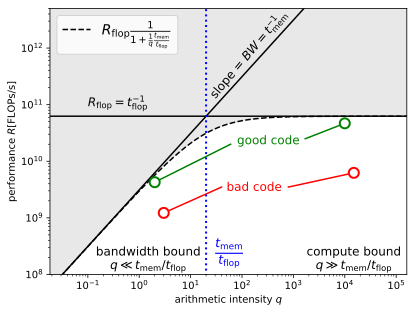
\includegraphics[width=0.6\linewidth]{figures/roofline.pdf}
\end{center}
\vspace{-2ex}
Real performance limited by
\begin{itemize}
\item cache hierarchy (additional memory references)
\item additional instructions
\end{itemize}
\end{frame}

%%%%%%%%%%%%%%%%%%%%%%%%%%%%%%%%%%%%%%%%%%%%%%%%%%%%%%%%%%%%%%%%%%

\begin{frame}
  \frametitle{Optimising solver performance}
  Requirements for fast solver
  \begin{itemize}    
    \item Efficient implementation (close to roofline)
    \item Optimal algorithm
    \begin{itemize}
      \item number of iterations
      \item small cost per iteration
    \end{itemize} 
  \end{itemize}
  Examples
  \begin{itemize}
  \item Gaussian elemination
  \begin{itemize}
    \item Convergences in single iteration
    \item Cost per iteration $\mathcal{O}(n^3)$
  \end{itemize}
  \item Richardson + Jacobi
  \begin{itemize}
  \item Requires multiple iterations
  \item Cost per iteration $\mathcal{O}(n)$
  \end{itemize}
  \item Conjugate gradient method, other preconditioner
  \begin{itemize}
  \item Reduce \# iterations
  \item Higher cost per iteration
  \end{itemize}
  \end{itemize}
\end{frame}

%%%%%%%%%%%%%%%%%%%%%%%%%%%%%%%%%%%%%%%%%%%%%%%%%%%%%%%%%%%%%%%%%%

\begin{frame}[fragile]
  \frametitle{Comparison of different solvers}
  \begin{center}
  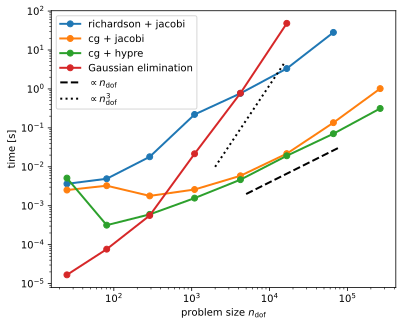
\includegraphics[width=0.6\linewidth]{figures/runtime_sparse.pdf}
  \end{center}
  \vspace{-1ex}
Solver configurations (tolerance {\footnotesize\verb`-ksp_rtol 1E-9`})
\begin{itemize}
 \item Gaussian elimination
  \item Richardson + Jacobi ({\footnotesize\verb`-ksp_type richardson -pc_type jacobi`})
  \item CG + Jacobi ({\footnotesize\verb`-ksp_type cg -pc_type jacobi`})
  \item CG + AMG ({\footnotesize\verb`-ksp_type cg -pc_type hypre`})
\end{itemize}
\end{frame}

%%%%%%%%%%%%%%%%%%%%%%%%%%%%%%%%%%%%%%%%%%%%%%%%%%%%%%%%%%%%%%%%%%

\begin{frame}
  \frametitle{Number of solver iterations}
\textbf{Total time}
$$
T_{\text{solve}} = n_{\text{iter}}\cdot t_{\text{iter}}.
$$
\begin{center}
\begin{tabular}{cccc}
  \hline
 $n_{\text{dof}}$ & Ric. + Jacobi & CG + Jacobi & CG + AMG\\
 \hline\hline
 25 & 3101 & 11 & 3 \\
 81 & 7959 & 23 & 5 \\
 289 & 14914 & 49 & 5 \\
 1089 & 32137 & 97 & 6 \\
 4225 & 33888 & 187 & 6 \\
 16641 & 37030 & 232 & 6 \\
 66049 & 129815 & 450 & 6 \\
 263169 & 447667 & 876 & 6 \\
\hline
\end{tabular}
\end{center}
\textbf{Observations}
\begin{itemize}
  \item Richardson + Jacobi: $n_{\text{iter}}\propto n_{\text{dof}}$
  \item CG + Jacobi: $n_{\text{iter}}\propto n_{\text{dof}}$
  \item CG + AMG $n_{\text{iter}} = \text{constant}$
\end{itemize}
\end{frame}

%%%%%%%%%%%%%%%%%%%%%%%%%%%%%%%%%%%%%%%%%%%%%%%%%%%%%%%%%%%%%%%%%%

\begin{frame}
  \frametitle{Time per iteration}
  \begin{minipage}{0.5\linewidth}
\begin{center}
  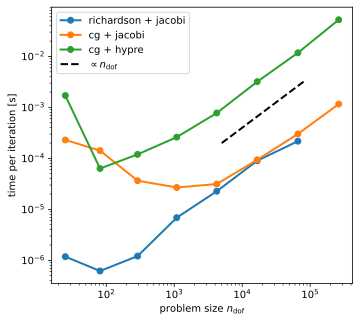
\includegraphics[width=\linewidth]{figures/time_per_iteration_sparse.pdf}\\
  {\footnotesize time per iteration $t_{\text{iter}}$}
\end{center}
\end{minipage}
\hfill
\begin{minipage}{0.39\linewidth}
\begin{center}
  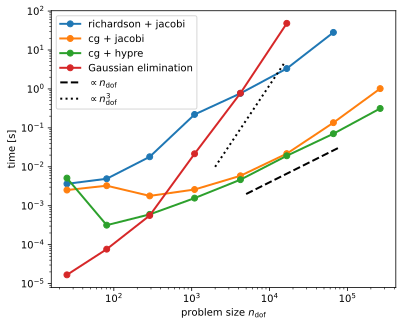
\includegraphics[width=\linewidth]{figures/runtime_sparse.pdf}\\
  {\footnotesize total time}
  \end{center}
\end{minipage}\\[2ex]
\textbf{Observations}
\begin{itemize}
\item $t_{\text{iter}}\propto n_{\text{dof}}$ 
\item $t_{\text{iter}}(\text{CG+AMG}) \approx 10\times t_{\text{iter}}(\text{CG+Jacobi})$ 
\item CG+AMG fastest due to small number of iterations
\end{itemize}.
\end{frame}

%%%%%%%%%%%%%%%%%%%%%%%%%%%%%%%%%%%%%%%%%%%%%%%%%%%%%%%%%%%%%%%%%%

\section{Parallel Computing}

%%%%%%%%%%%%%%%%%%%%%%%%%%%%%%%%%%%%%%%%%%%%%%%%%%%%%%%%%%%%%%%%%%

\begin{frame}
  \tableofcontents[currentsection]
\end{frame}

%%%%%%%%%%%%%%%%%%%%%%%%%%%%%%%%%%%%%%%%%%%%%%%%%%%%%%%%%%%%%%%%%%

\begin{frame}
  \frametitle{The need for parallel computing}
  Solve larger and larger problems $\Rightarrow$ more powerful computers\\[1ex]
  \textbf{Example} Met Office weather forecast
  \begin{itemize}
    \item Simulate evolution of state of the atmospheric
    \item Solve sparse linear systems of equations with $n_{\text{dof}}=10^6-10^9$
    \item 1000's of solves required for a typical 24h forecast 
  \end{itemize}
  \begin{center}
  \includegraphics[width=0.35\linewidth]{figures/runtime_sparse.pdf}
  \end{center}
  \begin{itemize}
    \item Optimal solver: $n_{\text{dof}}=0.26\cdot10^{6}$ $\Rightarrow$ $0.315 \text{s}$
  \item $n_{\text{dof}}=10^9$ unknowns $\Rightarrow$ $\frac{10^9}{0.26\cdot10^{6}}\times 0.3125\text{s} > 15 \text{min}$ 
  \item total time (solve only) $> 1000\times 15\text{min} = 10.4\text{days} \gg 24\text{hours}$
  \end{itemize}
  \end{frame}

%%%%%%%%%%%%%%%%%%%%%%%%%%%%%%%%%%%%%%%%%%%%%%%%%%%%%%%%%%%%%%%%%%

\begin{frame}
  \frametitle{Speedup through parallelisation}
  So far: all calculations performed by \textbf{single processor}\\[2ex]
  \textbf{Strategy}
  \begin{itemize}
    \item Split the problem into smaller chunks
    \item Solve each subproblem with a different processor \textbf{in parallel}
  \end{itemize}
  \begin{center}
  \includegraphics[width=0.75\linewidth]{figures/partitioned_mesh.pdf}
  \end{center}
  \textbf{Anticipated speedup}
  \begin{center}
  $P$ processors $\Rightarrow$ $P$ times faster code
  \end{center}
  \end{frame}

%%%%%%%%%%%%%%%%%%%%%%%%%%%%%%%%%%%%%%%%%%%%%%%%%%%%%%%%%%%%%%%%%%

\begin{frame}
  \frametitle{Parallel computers}
  
  \textbf{Modern supercomputers}
  \begin{itemize}
  \item Millions of compute cores
  \item perform $>10^{18}$ floating point operations per second (\textbf{ExaFLOP} performance)
  \item $10^6\times$ faster than our computer $R=6.3\cdot 10^{10}$ FLOPs
  \end{itemize}
  \href{https://top500.org/lists/top500/list/2025/06}{top500 list of supercomputers}\\[1ex]
  \textbf{Desktop computers, mobile phones}
  \begin{itemize} 
    \item typically have multiple processing units
  \end{itemize}
  \begin{center}
  $\Rightarrow$ need to exploit parallelism
  \end{center}
\end{frame}

%%%%%%%%%%%%%%%%%%%%%%%%%%%%%%%%%%%%%%%%%%%%%%%%%%%%%%%%%%%%%%%%%%

\begin{frame}
  \frametitle{Parallelisation}
  \textbf{Example:} domain decomposition for weather forecasting
  \begin{center}
  \includegraphics[width=0.75\linewidth]{figures/partitioned_mesh.pdf}
  \end{center}
  \begin{itemize}
     \item Distribute (meshed) domain between 4 processors 
     \item Each processor: solve equations of atmospheric fluid dynamics in parallel in its own local domain.
  \end{itemize}
  \begin{center}
  $\Rightarrow$ expect $4\times$ speedup
  \end{center}
\end{frame}

%%%%%%%%%%%%%%%%%%%%%%%%%%%%%%%%%%%%%%%%%%%%%%%%%%%%%%%%%%%%%%%%%%

\begin{frame}
  \frametitle{Parallelisation}
  \textbf{Example:} domain decomposition for weather forecasting
  \begin{center}
  \includegraphics[width=0.75\linewidth]{figures/partitioned_mesh.pdf}
  \end{center}
  \textbf{Challenges}
  \begin{itemize}
    \item Computations in different subdomains not independent
    \item BCs for "red" domain depend on computations in other subdomains
    \item Processors exchange information at regular intervals
  \end{itemize}
\end{frame}

%%%%%%%%%%%%%%%%%%%%%%%%%%%%%%%%%%%%%%%%%%%%%%%%%%%%%%%%%%%%%%%%%%

\begin{frame}
  \frametitle{Distributed memory parallelism}
  Conceptual approach to parallelisation
  \begin{center}
\includegraphics[width=0.5\linewidth]{figures/communication.pdf}
\end{center}
\begin{enumerate}
\item Each processor "owns" local part of the global problem
\begin{itemize}
  \item store \textbf{local data}\\
  ${}\qquad{}$ {\footnotesize $\Rightarrow$ mitigate memory constraints $\Rightarrow$ solve larger problems}
  \item perform computations on owned data
\end{itemize}
\item Processors communicate by \textbf{exchanging messages}
\end{enumerate}
\begin{description}
  \item[Mathematically]: \textbf{domain decomposition}
  \item[Computationally]: \textbf{distributed memory parallelism}
\end{description}
Other parallelisation approaches (not covered here):\\Shared memory, Threading, Vectorisation, mixed, \dots
\end{frame}

%%%%%%%%%%%%%%%%%%%%%%%%%%%%%%%%%%%%%%%%%%%%%%%%%%%%%%%%%%%%%%%%%%

\begin{frame}[fragile]
  \frametitle{Message passing interface}
  Exchange with the Message Passing Interface (MPI)
  (mpi4py in Python)
  \textbf{Example}
\begin{lstlisting}
import numpy as np
from mpi4py import MPI

comm = MPI.COMM_WORLD  # global communicator
rank = comm.Get_rank() # work out rank

# initialise data
data = np.zeros(4, dtype=int)
data[:] = rank + 1

print(f"BEFORE: rank {rank} has data", data)

# exchange data
if rank == 0:
    comm.Send(data, 1)
else:
    comm.Recv(data, source=0)

print(f"AFTER: rank {rank} has data", data)
\end{lstlisting}

\end{frame}

%%%%%%%%%%%%%%%%%%%%%%%%%%%%%%%%%%%%%%%%%%%%%%%%%%%%%%%%%%%%%%%%%%

\begin{frame}[fragile]
  \frametitle{Message passing interface}
  \textbf{Crucial idea}
  \begin{itemize}
    \item Both processors execute the \textbf{same source code}
    \item What exactly a particular processor does depends on value of variable \lstinline{rank}, which is different for each processor
  \end{itemize}
  \textbf{In the example}
  \begin{itemize}
  \item Each branch of the if-statement only executed by exactly on processor
  \item Each processor has own, local copy of array \lstinline{data}
  \item Data passed between processors with \lstinline{comm.Send()}, \lstinline{comm.Recv()}\\
    \textbf{Must execute both}
  \end{itemize}
\end{frame}

%%%%%%%%%%%%%%%%%%%%%%%%%%%%%%%%%%%%%%%%%%%%%%%%%%%%%%%%%%%%%%%%%%

\begin{frame}[fragile]
  \frametitle{Message passing interface}
Running the code
\begin{verbatim}
mpirun -n 2 python message_exchange.py

BEFORE: rank 0 has data [1 1 1 1]
BEFORE: rank 1 has data [2 2 2 2]
AFTER: rank 0 has data [1 1 1 1]
AFTER: rank 1 has data [1 1 1 1]
\end{verbatim}
\begin{itemize}
  \item Pair sends and receives
\item \lstinline{comm.Send()} can only complete once a corresponding \lstinline{comm.Recv()} has been executed
\item Danger of \textbf{deadlock}
\end{itemize}
\end{frame}

%%%%%%%%%%%%%%%%%%%%%%%%%%%%%%%%%%%%%%%%%%%%%%%%%%%%%%%%%%%%%%%%%%

\begin{frame}
  \frametitle{Parallel matrix-matrix product}
  \textbf{Example} matrix-matrix product
  $$C=AB$$
  \begin{itemize}
  \item $A$: $n\times m$ matrix
  \item $B$: $m\times r$ matrix
  \item $C$: $n\times r$ matrix
  \end{itemize}
  \textbf{Special case} matrix-vector product\\
  $r=1$ $\Rightarrow$ $B$ $\leftrightarrow$ vector $\vec{b}$
  $$\boldsymbol{y}=A\boldsymbol{x}$$
\end{frame}

%%%%%%%%%%%%%%%%%%%%%%%%%%%%%%%%%%%%%%%%%%%%%%%%%%%%%%%%%%%%%%%%%%

\begin{frame}
  \frametitle{Parallel matrix-matrix product}
  Distribute matrices between $P$ processors
  \begin{center}
\includegraphics[width=\linewidth]{figures/parallel_matmat.pdf}
\end{center}
$n\times m$ matrix: processor $p\in\{0,1,2,\dots,P-1\}$ stores rows $p\cdot n_{\text{local}}$ to $(p+1)\cdot n_{\text{local}}-1$\\[1ex]
\textbf{\# rows per processor}
$$
n_{\text{local}} = \frac{n}{P} \qquad\text{(assume that $P$ dives $n$)}
$$
\end{frame}

%%%%%%%%%%%%%%%%%%%%%%%%%%%%%%%%%%%%%%%%%%%%%%%%%%%%%%%%%%%%%%%%%%

\begin{frame}
  \frametitle{Parallel matrix-matrix product}
$\Rightarrow$ process $p$ stores
\begin{itemize}
\item $n_{\text{local}}\times m$ matrix $A_p$
\item $m_{\text{local}}\times r$ matrix $B_p$ ($m_{\text{local}} = m/P$)
\item $n_{\text{local}}\times r$ matrix $C_p$
\end{itemize} 
Split $A_p$ into $P$ (local) matrices $A_{pq}$ of shape $n_{\text{local}}\times m_{\text{local}}$\\[1ex]
\textbf{Matrix-matrix product}
$$
C_p = \sum_{q=0}^{P-1} A_{pq} B_q \qquad\text{for each processor $p=0,1,\dots,P-1$}
$$
\vspace{-4ex}
\begin{center}
\includegraphics[width=0.6\linewidth]{figures/parallel_matmat.pdf}
\end{center}
\vspace{-2ex}
$A_{pq} B_q$ = product of two $n_{\text{local}}\times m_{\text{local}}$ and $m_{\text{local}}\times r$ matrices

\end{frame}

%%%%%%%%%%%%%%%%%%%%%%%%%%%%%%%%%%%%%%%%%%%%%%%%%%%%%%%%%%%%%%%%%%

\begin{frame}
  \frametitle{Parallel matrix-matrix product}
  \textbf{Matrix-matrix product}
$$
C_p = \sum_{q=0}^{P-1} A_{pq} B_q \qquad\text{for each processor $p=0,1,\dots,P-1$}
$$
\vspace{-4ex}
\begin{center}
\includegraphics[width=0.6\linewidth]{figures/parallel_matmat.pdf}
\end{center}
  \textbf{Challenge}
  \begin{itemize}
    \item Each processor can compute the product $A_{pp}B_p$
    \item Computing $A_{pq}B_q$ for $q\neq p$ requires $B_q$ stored on different processor $\Rightarrow$ \text{Communication}
  \end{itemize}
\end{frame}

%%%%%%%%%%%%%%%%%%%%%%%%%%%%%%%%%%%%%%%%%%%%%%%%%%%%%%%%%%%%%%%%%%

\begin{frame}
  \frametitle{Parallel matrix-matrix product}
  \textbf{Algorithm: parallel matrix-matrix product}
  \begin{algorithmic}[1]
  \For{each processor $p=0,1,\dots,P-1$ in parallel}
  \State{Initialise $C_p \mapsto 0$}
  \State{Set $\widehat{B} \gets B_p$}
  \For{$q=0,1,\dots,P-1$}
  \State{$C_p \gets C_p + A_{p,(p+q)\;\text{mod}\;P} \widehat{B}$}
  \If{$q<P-1$}
  \State{Send $\widehat{B}$ to left neighbour $(p-1)\;\text{mod}\;P$}
  \State{Receive new $\widehat{B}$ from right neighbour $(p+1)\;\text{mod}\;P$}
  \EndIf
  \EndFor
  \EndFor
  \end{algorithmic}
\end{frame}

%%%%%%%%%%%%%%%%%%%%%%%%%%%%%%%%%%%%%%%%%%%%%%%%%%%%%%%%%%%%%%%%%%

\begin{frame}[fragile]
  \frametitle{Parallel matrix-matrix product}
  \textbf{Python implementation}
  \begin{lstlisting}
def parallel_matmul(A, B, C):
    comm = MPI.COMM_WORLD
    rank = comm.Get_rank()
    nproc = comm.Get_size()

    m_loc, _ = B.shape

    for q in range(nproc):
        C[:, :] += (
            q_ = (q + rank) % nproc
            A[:, q_ * m_loc : (q_ + 1) * m_loc] @ B[:, :]
        )
        if q < nproc - 1:
            comm.Sendrecv_replace(B, (rank - 1) % nproc)
    return C
  \end{lstlisting}
  Observe:
  \begin{itemize}
    \item "Owned" parts of matrices: \lstinline{A}, \lstinline{B}, \lstinline{C}
    \item \lstinline{comm.Send()} + \lstinline{comm.Recv()} $\rightarrow$ \lstinline{comm.Sendrecv_replace()}
  \end{itemize}
\end{frame}

%%%%%%%%%%%%%%%%%%%%%%%%%%%%%%%%%%%%%%%%%%%%%%%%%%%%%%%%%%%%%%%%%%

\begin{frame}
  \frametitle{Performance analysis}
  $$
C_p = \sum_{q=0}^{P-1} A_{pq} B_q \qquad\text{for each processor $p=0,1,\dots,P-1$}
$$
  Matrix-vector product $A_{pq}B_q$ 
  \begin{itemize}
\item $2n_{\text{local}}m_{\text{local}}r$ FLOPs
\item $n_{\text{local}} \times m_{\text{local}}$ + $m_{\text{local}}\times r$ memory reads (matrices $A_p$q, $B_q$)
\item $n_{\text{local}}\times r$ writes (matrix $C_p$)
\item Repeat $P$ times
  \end{itemize}
\textbf{Total cost}
$$
\begin{aligned}
T_{\text{compute}} &= \Big(2n_{\text{local}}m_{\text{local}}r\cdot t_{\text{flop}}\\
&\qquad+\;\; \left(n_{\text{local}}m_{\text{local}}+m_{\text{local}}r+n_{\text{local}}r\right)t_{\text{mem}}\Big)P\\
&=\frac{2nmr\cdot t_{\text{flop}}+(nm+mr+nr)t_{\text{mem}}}{P}
\end{aligned}
$$
\begin{center}
Runtime reduced by factor $P$ {\footnotesize(compared to sequential case)}
\end{center}
\end{frame}

%%%%%%%%%%%%%%%%%%%%%%%%%%%%%%%%%%%%%%%%%%%%%%%%%%%%%%%%%%%%%%%%%%

\begin{frame}
  \frametitle{Performance Analysis}
  \textbf{Communication overhead}
  Exchange $B_q$ $\Rightarrow$ $P-1$ messages of size $m_{\text{local}}\times r$\\[1ex]
  Cost for sending a message
  \begin{itemize}
  \item Startup cost (latency): $t_{\text{lat}}$
  \item Cost per word: $t_{\text{word}}$\\
  {\footnotesize(1 word = 64 bits = 8 byte = 1 double precison number)}
  \end{itemize}
  \textbf{Communication cost}
$$
\begin{aligned}
T_{\text{comm}} &= (P-1)\left(t_{\text{lat}} + m_{\text{local}}r\cdot t_{\text{word}}\right)\\
&= (P-1)t_{\text{lat}} + \frac{P-1}{P} mr\cdot t_{\text{word}}
\end{aligned}
$$
\end{frame}

%%%%%%%%%%%%%%%%%%%%%%%%%%%%%%%%%%%%%%%%%%%%%%%%%%%%%%%%%%%%%%%%%%

\begin{frame}
  \frametitle{Performance analysis}
  \textbf{Total cost} (memory access + FLOPs + communication)\\
$$
T(P) = T_{\text{compute}} + T_{\text{comm}} = \underbrace{\frac{2n^3 t_{\text{flop}}+3n^2 t_{\text{mem}}}{P}}_{A} + \underbrace{n^2 t_{\text{word}} + P t_{\text{lat}}}_{B}
$$
for $n=m=r$ and $P\gg 1$
\begin{itemize}
\item Term A: decreases with $P$
\item Term B: increases with $P$
\item Relative size $A/B$ depends on $P$ and problem size $n$ 
\item Usually $t_{\text{flop}} \ll t_{\text{mem}} < t_{\text{word}} \ll t_{\text{lat}}$ 
\end{itemize}
\end{frame}

%%%%%%%%%%%%%%%%%%%%%%%%%%%%%%%%%%%%%%%%%%%%%%%%%%%%%%%%%%%%%%%%%%

\begin{frame}
  \frametitle{Performance indicators}
  Analytical performance model only available for very simple algorithms\\
  $\Rightarrow$ \textbf{measurements} + \textbf{performance indicators}
 \begin{center}
  $T(P)$ = runtime on $P$ processors
 \end{center}
  Ideally: $T(P) = T(1)/P$ \\[1ex]
  \textbf{Parallel speedup}
$$
S(P) := \frac{T(1)}{T(P)} \le P = S^\star(P) \qquad\text{(ideal speedup)}
$$
\textbf{Parallel efficiency}
$$
E(P) := \frac{S(P)}{S^\star(P)} = \frac{T(1)}{P\cdot T(P)} \le 1,
$$
\end{frame}

%%%%%%%%%%%%%%%%%%%%%%%%%%%%%%%%%%%%%%%%%%%%%%%%%%%%%%%%%%%%%%%%%%

\begin{frame}
  \frametitle{Performance indicators}
  Parallel scaling, matrix-matrix product for different problem sizes $n$
  \begin{center}
  \includegraphics[width=\linewidth]{figures/parallel_scaling_measured.pdf}
  {\footnotesize (measured)}\\[1ex]
  \includegraphics[width=\linewidth]{figures/parallel_scaling_theory.pdf}
  {\footnotesize (theoretical performance model)}
  \end{center}
 
\end{frame}

%%%%%%%%%%%%%%%%%%%%%%%%%%%%%%%%%%%%%%%%%%%%%%%%%%%%%%%%%%%%%%%%%%

\end{document}

%%%%%%%%%%%%%%%%%%%%%%%%%%%%%%%%%%%%%%%%%%%%%%%%%%%%%%%%%%%%%%%%%%
